% Copyright (c) 2005-2009 Center for Urban Simulation and Policy Analysis,
% University of Washington.  Permission is granted to copy, distribute and/or
% modify this document under the terms of the GNU Free Documentation License,
% Version 1.2 or any later version published by the Free Software Foundation;
% with no Invariant Sections, no Front-Cover Texts, and no Back-Cover Texts.
% A copy of the license is included in the section entitled "GNU Free
% Documentation License".

% This is the root latex source file for the Opus and UrbanSim Users Guide.
% The guide is organized as a set of 'include' files, normally one file
% per chapter.  It uses the Python latex documentation standards and latex
% definition files -- see http://www.python.org/doc/current/doc/doc.html
% Also see the "Writing Documentation" chapter in this manual for more
% information.

% Each latex source file (including the 'include' files) should have
% the GNU Free Documentation License as a comment.

\documentclass{latex_files/manual}
\usepackage{amsmath, graphics, graphicx, rotating, html, upquote}

% this package causes the font encodings to include an _ (underscore)
% character -- this is useful because then searching the pdf document
% finds names with underscores in them.  (Otherwise the underscore is
% produced using a rule rather than a character and won't show up in
% searches.)
\usepackage[T1]{fontenc}
%\usepackage[ps2pdf]{hyperref}

\sloppy
\newcommand{\tight}{\itemsep 0pt}

\title{UrbanSim Version 4.1 \\
~\\
Reference Manual and Users Guide}

\author{The UrbanSim Project}

\authoraddress{Center for Urban Simulation and Policy Analysis \\
Daniel J. Evans School of Public Affairs \\
University of Washington \\
Box 353055 \\
Seattle, Washington 98195 \\
USA \\
% Put the real email address only in the pdf version (to avoid including
% a spam magnet in the html version).  A mangled version of the address
% (using "info (at) urbansim.org") is included in the html version by
% a parameter to the latex2html command
%begin{latexonly}
Email: \email{info@urbansim.org}
%end{latexonly}
}

\date{\today}
% replace \today with a real date (\date{April 1, 2000} ...} when this
% manual is ready for release so that reformatting doesn't cause a
% new date to be used.  For now, setting the date to \today during
% early editing makes it easier to handle versions.


% release version; this is used to define the \version macro
% omit the version unless this is a stable release -- for incremental
% versions just let the date identify the version
% \release{1.0.beta1}

% this tells \index to actually write the .idx file
\makeindex

% not (yet) used:
% \makemodindex                 % If this contains a lot of module sections.

\begin{document}

\maketitle

%% Copyright (c) 2005-2009 Center for Urban Simulation and Policy Analysis,
% University of Washington.  Permission is granted to copy, distribute and/or
% modify this document under the terms of the GNU Free Documentation License,
% Version 1.2 or any later version published by the Free Software Foundation;
% with no Invariant Sections, no Front-Cover Texts, and no Back-Cover Texts.
% A copy of the license is included in the section entitled "GNU Free
% Documentation License".

Copyright \copyright{} 2005--2009
Center for Urban Simulation and Policy Analysis,
University of Washington.  

Permission is granted to copy, distribute and/or
modify this document under the terms of the GNU Free Documentation License,
Version 1.2 or any later version published by the Free Software Foundation;
with no Invariant Sections, no Front-Cover Texts, and no Back-Cover Texts.
A copy of the license is included in the section entitled ``GNU Free
Documentation License''.



% \begin{abstract}
% abstract would go here, but we don't have one
% \end{abstract}

% The ugly "%begin{latexonly}" pseudo-environment suppresses the table
% of contents for HTML generation.
%
%begin{latexonly}
\tableofcontents
%end{latexonly}

\newcommand{\package}[1]{\index{opus packages!#1@\textit{#1} package} \textit{#1}}


% start the page numbering for the Part I page, so that it matches the
% actual pages (as shown when viewing the pdf file with Acrobat)
\setcounter{page}{6}
%\part{Overview of Opus and UrbanSim}\label{part-overview}
%\emph{This part under construction...}

three design dimensions (geographic level, degree of aggregation of agents, temporal dimensions); data required for each
%\section{Models}

The model architecture is adapted from the functional design of SAM,
and also informed by the development of OPUS and UrbanSim. The
functionality in SAM focuses on the allocation of land use by
sector to grid cells, from aggregate information at a mid-level
geography such as MPAs.  By reference to the UrbanSim model system,
this functionality is approximately equivalent in purpose to the
real estate development model component of UrbanSim, with some key
differences.  UrbanSim attempts to include a complete representation
of the real estate market, with occupants (consumers: households
and jobs), buildings and land (suppliers: developers and property
owners), and prices (markets: hedonic regressions representing the
interaction of suppliers and consumers).

The architecture for the model system proposed for AZ-SMART is
based on a 3-year plan, and incorporates the complete market
representation as in UrbanSim, and a multi-level geography and
model system.  We describe this in the Full Model System subsection
 below, and then focus on a Phase 1 Model System in the subsequent
 section.

\subsection{Full Model System}
The full model system proposed for AZ-SMART involves some
hybridization and extension of elements of UrbanSim and SAM-IM.
Below we itemize the core elements of the full model system
architecture.

\begin{itemize}

\item \emph{Land-Structure-Occupant Accounting}: The full market
representation and explicit representation of and accounting of
Land-building-occupant objects and their relationship is proposed
for the full model architecture.

\item \emph{Parcels and Buildings}: Land could be represented by
parcels, land use polygons, or cells, but it is expected that
the parcel concept would be used as the principal representation
of land, and that in areas that do not have parcel data available,
land use polygons could be used in a way that treats them as
equivalent to (possibly large) parcels.  Note that there are many
to one relationships from buildings to land and from occupants to
building.  That is, a building may contain multiple occupants,
and a parcel (or land use polygon) may contain multiple buildings.
In the event that building data is not available, it could be
imputed, to preserve a consistent data model.

\item \emph{Development Projects, Sites and Templates}: Development
 Projects are proposed as a higher-level construct to represent
 one or more parcels that form a coherent single development
 project, such as single-family housing subdivision, or a shopping
 center complex.  These development projects will deal both with
 known \emph{development projects} which the user wishes to
 incorporate into the simulation, and also development projects
 predicted by the simulation and assigned to \emph{development
 sites}.  For predicted development projects, a set of pre-defined
  \emph{development templates} provide a set of configurations of
  development that include at a minimum the mix of building types
  (land uses), density, size and timetable for development.

\item \emph{Multi-level Model}: The full model system would use
a multi-level approach, incorporating parcels as the lowest level
(buildings are linked to parcels), and for the forseeable future,
one higher level geography to represent an intermediate geography
between the county and the parcel.  Traffic Analysis Zones (TAZ)
are proposed as the basis for this mid-level geography in the full
 model, simplifying the interface with the travel model system.
 There are behavioral and practical reasons for using a two-level
 geography in the model system.  Behaviorally, it is based on the
 expectation that consumers looking for a location (e.g. a household
  searching for a house) compare neighborhoods, and select properties
  to examine based on their assessment of the neighborhoods. In
  practical terms, the two-level geography provides a more convenient
  way to interface models in a modular way, for example to interface
  the travel model system, or to run the model system for corridor or
  area studies where more detail is needed in a subset of the planning
  region and less is needed outside of this focus area.

\item \emph{Microsimulation}: The proposed architecture is based on
explicit representation of the agents and objects being modeled at a
microscopic level.  Parcels, buildings, businesses (or jobs),
households, and eventually, persons (for supporting activity-based
travel models and workplace choice models and individual-level
accessibility calculations).

\item \emph{Temporal Dynamics}: The model system would be able to
use a specified time interval, such as 5-year or 1-year steps,
between which it would simulate changes to the state of each object
and agent in the system (construction of new buildings or conversion
of existing ones, movement of households and businesses from one
location to another, creation of new households or businesses).

\item \emph{Models and Interface}: A set of models will be interfaced
through a common data store, and managed by a Model Coordinator that
controls their execution and implements events (changes to the data)
proposed by models.  The individual models would be the following:

\begin{itemize}
\item Demographic Transition (Region): Reconciles the control totals
of population (by household type) with the database - adding households
to the database or removing them if a household type is declining.
\item Employment Transition (Region): Reconciles the control totals
of employment (by sector) with the database - adding businesses (jobs)
to the database or removing them if a sector is declining.
\item Development Project Transition (Region): Reconciles the total
demand for real estate by type, including the results of the Demographic
and Employment Transition models, with the existing stock of real estate,
by generating proposed Development Projects until vacancy rates reach
long-term structural levels.
\item Household Relocation (Region): Predicts whether a household will
move from their existing residence during the next time step.
\item Business Relocation (Region): Predicts whether a business  (job)
will move from their existing location during the next time step.
\item Household Location (TAZ and Parcel): Predicts the building that
a new or moving household will choose from among the set of buildings
with a vacanct unit.
\item Business Location (TAZ and Parcel): Predicts the building that a
new or moving business (job) will choose from among the set of buildings
with sufficient vacanct space.
\item Parcel Subdivision (Parcel): Predicts the number and size of
parcels to create from a large parcel that is to be subdivided to create
a development project. Depending on whether the project is known or
predicted this will use information provided in the development project
description or drawn from a development template.
\item Parcel Aggregation (Parcel): Combines adjacent parcels to create
a \emph{development site} suitable to place a development project.
\item Demolition (Building): Removes existing buildings based on age
and other characteristics that would indicate a high probability to
convert to another use or be abandoned.
\item Development Project Location (Development Site): Predicts the
development site chosen to locate a development project.
\item Building Development Model (Parcel): This would be based on the
Development Velocity Model, and predicts the construction of individual
buildings on parcels within a development project.
\item Real Estate Price Model (Building): This will predict the price
per unit (or sqft) for each type of real estate at each location (parcel).
\item Simplified Travel Model (TAZ): An abbreviated travel model with
just a.m. peak, and other simplifications to provide a relatively
high-speed regional travel model to use in intermediate years preceding
the target year for the regional transportation plan.
\end{itemize}
\end{itemize}

The models proposed for implementation in Phase 1 of this project are
described in greater detail in the following section.

\subsection{Phase 1 Model System}
Phase 1 of the AZ-SMART project focuses on the allocation of land use
sectors, essentially the real estate development process.  The plan
for Phase 1 is to focus on the real estate development components of
the full model system described in the preceding section, and to
suppress or use only simple 'stub' models for the remaining models
in the full system.  The objective is to provide the functionality
that is provided now by SAM, but in an implementation that is a
very big step towards a fully integrated market simulation model
system such as UrbanSim, and incorporating valuable innovations
such as the management of known development projects, and the use
of an intermediate level geography such as RAZ as the basis for
control totals for allocation to parcels (or land use polygons).

The following models would be the focus of model development in Phase 1:

\begin{itemize}
\item Parcel Subdivision (Parcel)
\item Parcel Aggregation (Parcel)
\item Development Project Location (Development Site)
\item Building Development Model (Parcel)
\end{itemize}

The following models would be implemented for completeness, but would
use only the simplest specification, to allow completeness.  For example,
the household location choice model could use an empty specification,
which would randomly allocate the household control total for a RAZ to
the housing units that have been developed on parcels in the RAZ.

\begin{itemize}
\item Demographic Transition (RAZ)
\item Employment Transition (RAZ)
\item Development Project Transition (RAZ)
\item Household Location (Parcel)
\item Business Location (Parcel)
\end{itemize}

The components of the full model system would be deferred until after Phase 1:

\begin{itemize}
\item Demolition (Building)
\item Real Estate Price Model (Building)
\item Simplified Travel Model (TAZ)
\end{itemize}





The model architecture has the following steps, using a 5-year time interval:

=== Determine Quantity of Development Needed ===

* Translate mid-level model predictions of population and employment by RAZ (or other mid-level geography) into predicted demands for housing units and land area of non-residential uses by type.
** This would be done using average density and occupancy assumptions.

=== Determine Development from Active Projects ===

* Compute the quantity of development expected in a RAZ (or other mid-level geography) for each land use sector, based on the velocity within Active Development projects.

* Assign the development generated by Active Development Projects to the cells within those developments.

=== Determine Eligible Development Sites ===

* Evaluate cells with vacant land to determine what kinds of development would be permitted on them according to the development constraints represented by Planned Land Use and other constraints (slopes, etc).  This applies development constraints in order to produce Eligible Vacant Lands for development.

* Evaluate potential availability of Redevelopment Districts for new development.

* Generate 'Development Sites' from 'patches' of available land suitable for development.  These are areas formed by contiguous cells eligible for development for a particular land use sector, and would serve as a counterpart to the polygons digitized by users for planned and active development projects.  They would allow the comparable representation of Development Sites from all sources.

=== Assign Development Projects to Development Sites ===

* Use 'Development Sites' as the candidate set of locations for new development within the RAZ.

* Generate a set of proposed 'Development Projects' that would fill the gap in the RAZ between the development that is generated by evaluating the velocity of Active Development Projects and the quantity required to meet the RAZ control totals.

* Compute logit model probability that a Development Project in a RAZ will choose one of the available candidate Development Sites.

** Compute variables used in utility (scoring function)
** Multiply variables by their coefficients
** Compute utility
** Compute probability

* 'Choose' a Development Site for each Development Project to be located based on the logit probabilites.  Specifically, draw a random number and compare it to the cumulative probability distribution across the alternative Development Sites.  Choose the site that the random number falls within (the choice pattern will be proportional to the logit probabilities).  Ensure that the capacities of the sites are respected: if a Development Project is too big for a site, exclude it from consideration.

* Once a Development Site is chosen for a Development Project, assign the Development Project to the Development Site, and set the Development Project status to 'Active', so it becomes part of the set of Active Development Projects that will be used to generate development at the beginning of each period.

* Generate initial development of the newly selected project sites for the current time period based on the predicted or stored development velocity.

* Compare generated development to that required to meet control totals.  Add more development if necessary.

=== Iterate over RAZs (or other geography) and Allocate Unplaced Development Projects ===

* Once allocation of all development in a RAZ or other mid-level geography is completed, process the next RAZ.

* If not all development could be allocated in a RAZ, accumulate unmet demand within a higher level geography to be processed in a final iteration.

* If needed, allocate unmet demand from higher level (MPA for example), to Development Sites as above.

=== Process Submodels and Interface to Other Models ===

* Once the core allocation model is finished,

** Run any needed 'Sub-models' for post-processing to create inputs to Travel Model
** Launch Travel Model run if this is configured for a scenario
** Resume model at next time step if this is configured for a scenario.

=== Generate Indicators and DataSets ===
As needed, once the model is completed on a Scenario:

* Configure indicators to produce from results, and the format for them:
** Tables
** Maps
** Charts
(Petya says:)'' Can we use the indicators to generate or edit feature classes and then use ArcMap to see the results? I would like whenever possible to organize the indicators in appropriate feature classes instead of keeping them in non-spatial columns of tables''''''


%\part{Opus and UrbanSim User Guide}\label{part-user-guide}
%% $Id: installation.tex,v 1.85 2007/06/01 23:49:22 borning Exp $

% Copyright (c) 2005-2007 Center for Urban Simulation and Policy Analysis,
% University of Washington.  Permission is granted to copy, distribute and/or
% modify this document under the terms of the GNU Free Documentation License,
% Version 1.2 or any later version published by the Free Software Foundation;
% with no Invariant Sections, no Front-Cover Texts, and no Back-Cover Texts.
% A copy of the license is included in the section entitled "GNU Free
% Documentation License".

\chapter{Installation}
\label{chapter:installation}

\index{installation}

Instructions for installing Opus and UrbanSim are available in html
format.  

\begin{itemize}

\item The instructions for the latest version are online at
\url{http://www.urbansim.org/docs/installation}.

\item If you have downloaded Opus from the CUSPA subversion repository, the
instructions for the version installed on your system can be found in the
directory \file{opus_docs/installation/} in your Opus workspace (start
with \file{index.html}).

\item If you have downloaded Opus as a zip file, the instructions for the
version installed on your system can be found in the directory
\file{docs/installation/} in the directory into which you unzipped the
contents (start with \file{index.html}).

\end{itemize}

Opus and UrbanSim are intended to be platform-independent.
\index{platform-independence} We have successfully installed and used the
system under the Windows, \windowsindex Linux, \linuxindex and Macintosh
\macintoshindex operating systems. These installation directions have been
tested with Windows XP, \windowstestindex SuSe Linux, \suseindex
\linuxtestindex and Macintosh OS X Version 10.4.5 \macintoshtestindex with both
PPC \index{PPC} and Intel \intelindex{} processors.

\index{Opus!dependencies}
\index{UrbanSim!dependencies}
\index{dependencies}
\index{supporting software}
\index{installation!installing supporting software}
Opus and UrbanSim rely on numerous other open-source systems, in particular
MySQL, Python, and a non-trivial set of Python packages.  Opus and UrbanSim
work with Python~2.4.3 or higher, \pythonversionindex and with
MySQL~5.0 or 4.1.18.\mysqlversionindex

% LocalWords:  borning UrbanSim IDEs XP SuSe ActivePython pre YaST devel PyDev
% LocalWords:  IDE plugin CVS Pydev PYTHONPATH mpkg MySQL SQL UW mysql mysqld
% LocalWords:  YaST's Runlevel Miktex FinkCommander tetex pdflatex TeXlipse sw
% LocalWords:  matplotlib utens cd sudo ln os plist xvfz gz py gcc Xcode url eg
% LocalWords:  XcodeTools numpy README config sourceforge BuildingMatplotlib
% LocalWords:  txt Darwinports PyXML xml dom RPy OpenEV IDE's init localhost un
% LocalWords:  MYSQLHOSTNAME MYSQLUSERNAME username urbansim MYSQLPASSWORD cvs
% LocalWords:  MacOSX bashrc unix extssh loc formulae pdf myfile tex userguide
% LocalWords:  makeindex socha PPC mysqlcc msi hostname FWTools 
% LocalWords:  uber AllTests OpenEv CSE yourname ber psrc MPO
% LocalWords:  CUSPA Uninstalling uninstall atlantis subpackages
% LocalWords:  subpackage Versioning CUSPA's synch DrPython

%%% Local Variables:
%%% mode: latex
%%% TeX-master: "userguide"
%%% End:

%% Copyright (c) 2005-2009 Center for Urban Simulation and Policy Analysis,
% University of Washington.  Permission is granted to copy, distribute and/or
% modify this document under the terms of the GNU Free Documentation License,
% Version 1.2 or any later version published by the Free Software Foundation;
% with no Invariant Sections, no Front-Cover Texts, and no Back-Cover Texts.
% A copy of the license is included in the section entitled "GNU Free
% Documentation License".

\chapter{Using the UrbanSim System}
\label{chapter:using-urbansim}
%
The latest incarnation of UrbanSim, UrbanSim 4, is implemented as a
set of packages in Opus. Package \package{opus_core} provides
general functionality, \package{urbansim} contains everything around
land use models, package \package{opus_emme2} is an
Opus wrapper to the travel model EMME/2.\index{emme/2}

\section{Running a Simulation}
%
\subsection{Support for Production Runs}
The ``Run Manager''\index{Run Manager} is a set of user functionality
provided by the \file{run_manager} directories in
the \package{opus_core} and \package{opus_core.services} packages
provide support for specifying, starting, re-starting, and
processing ``production`` runs. \index{production runs} Such a
system is necessary to deal with the long run times for such a model
\modelsindex system, and the large amount of data each run produces.
A 30-year simulation of the Puget Sound Regional Council's (PSRC)
\psrcindex dataset with their EMME/2 \index{emme/2} travel model, for
instance, takes about 5 days \index{simulation!run time} to complete
and creates about 14 GB of cache data. \index{cache!size of}
\index{simulation!space used by}  These numbers are for a computer
with dual 3.2 GHz Intel
Xeon processors and 4 GB of RAM running
Windows XP Professional. The PSCS dataset
  contains about 800,000 gridcells, 1.3 million
households, and 1.8 million jobs in the initial year. Each UrbanSim
year takes about 1.5 hours to simulate, and each travel model run,
done every 5 years, takes around 12 hours to simulate.

Here are some of the things Run Manager \runmanagerindex helps us do:
\begin{itemize}
  \item Define a run configuration, including what models to run, what years to
  run, etc.
  \item Start a production run.
  \item Monitor the status of all production runs.
  \item Re-start a production run when something goes wrong.
  \item Compute indicators on the results of a production run, including runs
  that are still simulating.
  \item Inspecting specific dataset values from any year of the simulation,
  as when diagnosing problems.
  \item Manage consistency regarding the availability and status of production runs.
\end{itemize}

\subsection{Run Management}
\label{sec:run-manager}
%
Opus contains a set of scripts that simplify the
process of starting and restarting a set of simulation runs.

At the moment, these scripts are a set of command line applications, or tools, in the
\file{opus_core/tools} directory.  They use a database as the central
repository for coordination and context infomation for run managment, by
default called \verb|services|.  If you don't have this database, create it
(you need to do this from within the \file{opus_core/tools}
directory):

\begin{verbatim}
python create_services_database.py
\end{verbatim}
This creates the database named \verb|services| on the \verb|localhost|
database server using the user name and password specified in the
\verb|MYSQLUSERNAME| \mysqlusernameindex and \verb|MYSQLPASSWORD| \mysqlpasswordindex environment variables. \environmentvariablesindex To use a
different host for the database server, include the \verb|--hostname|
option. To use a different database name, include the \verb|--database|
option:

\begin{verbatim}
python create_services_database.py --hostname myhost.mydomain --database
myservices
\end{verbatim}

All scripts described below print a help message when called with the
\verb|-h| or \verb|--help| option.

\subsubsection{Start a simulation using a Python Dictionary Configuration}
\index{start a simulation}

The configuration for a simulation is specified by a configuration object.
Previously, a configuration was specified as a Python dictionary, and we
describe the older option in this section.  We are transitioning toward
specifying configurations using an xml project file for use with the Opus
GUI--- see Section \ref{sec:start-simulation-xml} for information on
starting a simulation using an xml configuration but still from the command
line.  In both cases, the configuration is used to specify different parts
of the simulation, such as the years in which to run UrbanSim, what
UrbanSim models to run each year, what types of development
projects exist, how to configure each type of development project,
etc. See, for instance, the run configuration in
\verb|seattle_parcel/configs/baseline.py| (Python dictionary version) or
\verb|seattle_parcel/configs/seattle_parcel.xml| (xml version).

To use the dictionary version of a configuration, the start_run tool
requires that the referenced configuration Python module either (a) defines
a class (e.g. SubsetConfiguration) in a file whose name is
subset_configuration.py, or (b) defines a run_configuration object that is
the configuration object.  In the first case, the class name is the
CamelCase version of the lowercase_with_underscores file name.  \emph{(The
  preferred method is to define a class.)}

To start a simulation using a dictionary-based configuration, use the
script \verb|start_run| with the desired configuration.  First change to 
the directory \verb|opus_core/tools| and execute:
\begin{verbatim}
python start_run.py -c psrc.configs.subset_configuration
\end{verbatim}

Note that the configuration here is specified as it would be in a Python
``import'' statement.

If the \verb|services| database was created using the \verb|--hostname| and/or
\verb|--database| option, you will need to include these options in
\file{start_run.py} as well.  Use the \verb|--help| option to see
\verb|start_run|'s possible command line parameters.

The \verb|creating_baseyear_cache_configuration| entry in the configuration
contains the information specifying the location of the baseyear inputs.  
If \verb|cache_from_mysql| is \verb|True|, the inputs are taken from
the MySQL database specified in the \verb|input_configuration| entry. 
Otherwise, the inputs are taken from the baseyear cache specified in the
\verb|baseyear_cache| entry.  When the inputs are taken from MySQL, they are
used to create a baseyear cache stored in the directory specified by the
\verb|cache_directory| entry, or, if that entry is missing, from an directory
whose name encodes the date-time of the simulation request and is created in the
directory specified by the \verb|cache_directory_root| entry.  

For large amount of data, copying from MySQL to a baseyear cache takes much
longer than creating a new baseyear cache from an existing baseyear cache.  

Option \verb|--directory-to-cache| \index{cache!getting input from existing cache}
can be used to turn off the caching. It takes as argument the directory name
from which data are copied to the new basyear cache. With
the option \verb|--years-to-cache| one can control specific years to be
copied. The option takes as argument any python expression that returns a list
of years. These two options overwrite entries in the configuration that control
this behaviour.

\subsubsection{Start a simulation using an XML Configuration}
\label{sec:start-simulation-xml}

To start a simulation using an xml configuration from the command line, use
the script \verb|start_run| with the desired configuration.  Change to the
directory that holds the Opus source code and execute:
\begin{verbatim}
python opus_core/tools/start_run.py -x seattle_parcel/configs/seattle_parcel.xml 
       -s Seattle_baseline
\end{verbatim}
(typed all on one line).

Notice that the \verb|-x| option takes a path to the file with the xml
configuration.  Since xml configurations can hold multiple scenarios, the
scenario name must also be specified using the \verb|-s| option.

This same xml configuration can also be used with the Opus GUI ---
documentation on the GUI is forthcoming.

\subsubsection{Restart a simulation}
\index{restart a simulation}
If you halt a run or it fails, you can restart it at the beginning of any year.
To restart the run with \verb|run_id| 42 at the beginning of year 2005, do:

\begin{verbatim}
python restart_run.py 42 2005
\end{verbatim}
Again, options \verb|--hostname| and \verb|--database| must be included
if non-default values are used.  Note that the above command will delete any
simulation cache \simulationcacheindex directories for years 2005 onward, since
this information is no longer valid once the simulation is restarted at the
beginning of 2005.

If the 2005 travel model failed and you want to restart in 2005 but not re-run
the UrbanSim models, use the \verb|--skip-urbansim| option:

\begin{verbatim}
python restart_run.py 42 2005 --skip-urbansim
\end{verbatim}

If the 2005 travel model succeeded, and thus wrote its output to the 2006
simulation cache \simulationcacheindex directory, but you need to restart in year 2006, use the
\verb|--skip-cache-cleanup| option:

\begin{verbatim}
python restart_run.py 42 2006 --skip-cache-cleanup
\end{verbatim}

\subsubsection{Create Baseyear Cache}
\label{sec:run-manager-baseyearcache}
%
One can explicitely create a baseyear
cache\index{cache!getting input from existing cache} from
the base year database which can be then used for simulation runs. The script
needs a configuration module passed as an argument. The services database is
not used by the script. If the desired module is located at
\file{psrc/configs/subset_configuration.py} under one of the paths found in the
PYTHONPATH environment variable, the command

\begin{verbatim}
python create_baseyear_cache.py psrc.configs.subset_configuration
\end{verbatim}
caches the database defined in the \verb|subset_configuration| configuration into a baseyear
cache. The \file{create_baseyear_cache} file is located in
the \file{opus_core/tools/} directory, and the above command should be
run from the same directory. An option \verb|--cache-directory|
can be used to pass the directory to be cached into. Alternatively, this can be
specified in the configuration as an entry \verb|'cache_directory'|. See also
Section~\ref{sec:configuration} for configuration and cache control options.

\subsection{What Happens When Running a Simulation?}
\label{sec:run-manager-tasks}
Here are the steps that occur when you start a run via the \verb|start_run|
script:

\begin{itemize}
  
\item \index{cache!unrolling development_event_history}\index{Unrolling 
development_event_history}\index{development_event_history!unrolling} If 
required, it copies all of the tables from the baseyear database specified by 
the configuration into the baseyear cache and then creates a
set of pre-baseyear \verb|gridcells| tables by unrolling the
\verb|develoment_event_history| data.

The unrolling processes all records in the \verb|development_event_history| 
table.  It starts with the most current year of records, and moves backward in 
time.  For this description, assume that the baseyear is 2000.  The unrolling 
process first loads the gridcell dataset for year 2000.  For each 
\verb|develoment_event_history| record with \verb|scheduled_year| for the prior 
year (e.g. for 1999) it substracts from the gridcells any development by that 
event (e.g. \verb|residential_units|).  Values that go negative are set to 
zero.  Once all events for this year have been ``undone'', the unrolling 
process writes the modified gridcell dataset to the prior year, e.g. to 1999. 
This process is repreated for each year with data in 
\verb|develoment_event_history|.

If you only want 10 years of data to be unrolled, only put those years of data
into your \verb|develoment_event_history| table.

\item Alternatively, it copies files from a previously used baseyear cache into
the baseyear cache for the current run (including the

\item It adds a row to the \verb|run_activity| table in the \verb|services|
database, using a new \verb|run_id| value unique to this run. In order to help
match runs with their cache directory, the name of the cache directory begins
with the \verb|run_id| value, e.g. \file{run_342.2006_04_25_09_40}.

\item For each year in the set of years specified in the configuration:
  \begin{itemize}
  \item Stores to the cache a pickled version of the configurations for that
  year.
  \item Forks a new process to run the set of UrbanSim models for this year.
  The set of models to be run is specified by the configuration. Using a
  separate process helps reduce memory usage, \index{Memory!Using separate
  process} and helps reduce the impact of problems such as memory leaks.  This
  process writes a log file named, e.g., \file{year_2003_log.txt}.
  \item Run the EMME/2 \index{emme/2} travel model for this year, if specified by the travel
  model's configuration.  The set of steps to run for the travel model is fully
  specified by the \verb|'models'| section of the
  \verb|'travel_model_configuration'|. Typically, it includes a preparation step
  that prepares travel model inputs from the UrbanSim data, a step that
  actually runs the travel model, and one or more steps to puts the results of
  the travel model into the \verb|travel_data| dataset for the current year, so
  the data is visible to the UrbanSim models in that and following years.  Each
  model step is done in a separate process.  The log for the running of the
  model is written to a file named, e.g., \file{emme2_2005_log.txt}.
  \end{itemize}
  \item The run activity table includes status information about the run.  If
  the simulation succeeds, it will add another row to the run activity
  indicating it is done.  If the simulation fails, it will add a row indicating
  that.  The run activity also contains a copy of the configuration, which is
  used when restarting a run.
  \item Whenever a row is added to the \verb|run_activity| table, a row is
  either added or updated in the \verb|available_runs| table in the
  \verb|services| database. This table has a single row per run and records the
  row's current state and information.
\end{itemize}

\section{Configurations}
\label{sec:configuration}
%
A run configuration is a specification of what parts to use in the simulation
and how to configure each part.  Parts include the list and order of models to
run, where to get the input values, where to store the output data, what years
to simulate, what tables to store into the UrbanSim baseyear and simulation
caches\simulationcacheindex, etc. Each of these parts in
turn may be configurable.  The configuration for a travel model, for instance,
may specify which values to use from the land use models, and what travel model
results to extract in order to use them in the land use models. 

Configurations are used in many places in Opus.  Typically, they are specified
via a Python dictionary that then is used to create an instance of the
\class{Configuration} class.

\subsection{Run Manager Configuration}
\label{sec:run-manager-configuration}
%

UrbanSim can be started via the ``Run Manager'' \runmanagerindex (see
Section~\ref{sec:run-manager}) which is controlled by a user-defined
configuration. The following code contains a fully specified configuration
that influences behaviour of the run manager. \runmanagerindex Mandatory entries and default
values for optional entries are marked in the comments. The actual values for
the listed entries are only examples.

\emph{Note: we are in the process of splitting the following configuration
information into separate parts.  Once we are done with that refactoring,
we will update the documentation to the new arrangement.}

\mysqlhostnameindex\mysqlpasswordindex\baseyearcacheindex
\begin{verbatim}
from opus_core.configurations.database_configuration import DatabaseConfiguration
from opus_core.configurations.baseyear_cache_configuration \
    import BaseyearCacheConfiguration
    
from urbansim.configurations.creating_baseyear_cache_configuration \
    import CreatingBaseyearCacheConfiguration


run_configuration = {
    'model_system':'urbansim.model_coordinators.model_system', # mandatory
    'description':'baseline with travel model',      # default: 'No description'
    'cache_directory':'d:/urbansim_cache/',	         # mandatory
    'creating_baseyear_cache_configuration': CreatingBaseyearCacheConfiguration(
        # default: 'urbansim_tmp'+random string
        cache_directory_root = 'd:/urbansim_cache',

        # mandatory
        cache_scenario_database = 'urbansim.model_coordinators.cache_scenario_database',

        cache_from_mysql = False, # default: True

        # mandatory if 'cache_from_mysql' is False
        baseyear_cache = BaseyearCacheConfiguration(
            # mandatory for this block
            existing_cache_to_copy = 'd:/urbansim_cache/run_397.2006_05_23_18_21',
            
            # default: all years in 'existing_cache_to_copy'
            years_to_cache = range(1996,2001)
            },

        tables_to_cache = [ # default: []
            'gridcells',
            'households',
            'jobs',
            'zones'
            ]

        tables_to_cache_nchunks = { # default: each table defaults to 1
            'gridcells':2,
            },

        tables_to_copy_to_previous_years = { # default: no copied tables
            'development_type_groups':1996, # table name and year to put it in
            'development_types':1996,
            'development_type_group_definitions':1996,
            'urbansim_constants': 1996,
            },
        ),
\end{verbatim}

% long script split into two parts since it won't fit on one page

\begin{verbatim}
    'input_configuration': DatabaseConfiguration(    # mandatory
        host_name = os.environ['MYSQLHOSTNAME']      # mandatory
        user_name = 'urbansim',                      # mandatory
        password = os.environ['MYSQLPASSWORD'],      # mandatory
        database_name = 'PSRC_2000_baseyear',        # mandatory
        )
    'output_configuration': DatabaseConfiguration(   # default: No output
                                                     #     configuration
        host_name = os.environ['MYSQLHOSTNAME']      # mandatory for this block
        user_name = 'urbansim',                      # mandatory for this block
        password = os.environ['MYSQLPASSWORD'],      # mandatory for this block
        database_name = 'PSRC_2000_output',          # mandatory for this block
        },
    'base_year': 2000,                               # default: read from table
                                                     #     'base_year' in
                                                     #     'db_input_database'
    'years': (2001, 2030),                           # mandatory
}
\end{verbatim}
The \verb|'model_system'| entry is the full Opus path to the model system that
will be used by the run manager to run/estimate a set of models.

The \verb|'cache_scenario_database'| entry is the full Opus path to the class to use to
create a baseyear cache from the baseyear data in the MySQL database.  The
\verb|'urbansim.model_coordinators.cache_scenario_database'| version creates  both the
baseyear cache, and unrolls the gridcell data to populate prior years with the
gridcell dataset (see Section~\ref{sec:run-manager-tasks}).

Entry \verb|'creating_baseyear_cache_configuration'| contains the configuration
for creating the baseyear cache.

Entry \verb|'cache_directory_root'| is the root directory where data should be
cached during processing. The actual cache directory is created by adding
the run number and date-time string to this directory.

The \verb|'input_configuration'| is a DatabaseConfiguration object
that determines the MySQL \mysqlindex database with the base year
data.

Entry \verb|'output_configuration'| is a DatabaseConfiguration
object that determines the MySQL \mysqlindex database into to which
to write any database tables related to the results of the
simulation run.  Now that indicators are computed from the attribute
cache, the output database is only needed if you wish to use the SQL
indicators.  Before starting the simulation, the run manager will
remove any tables in the output_database, so be sure it doesn't
contain information you want to keep.

Entry \verb|'years'| determines for what
years the simulation should run as a tuple with first and last year to run.

By default, the run manager \runmanagerindex caches all tables from the input database into the
binary baseyear cache on which then the simulation runs. If
only selected tables should be cached, they can be put into
\verb|'tables_to_cache'|. Note that the simulation itself then does not use the
database anymore, all data are retreived from baseyear cache
and written to the simulation cache \simulationcacheindex.  That means, if the
entry \verb|'tables_to_cache'| is used, the user must ensure that it contains
all tables that are used by the simulation.

If a database table is so large that Python runs out of memory when copying it
to cache, you can reduce memory usage (but increase the time it takes to cache
the data) by increasing the number of ``chunks'' in which the dataset's 
attributes are read from the table. \index{Memory management!When caching data
from input store}\index{Memory management!tables_to_cache_nchunks@\texttt{tables_to_cache_nchunks}} By
default, all attributes of a table are read in a single chunk. Setting the
\verb|'tables_to_cache_nchunks'| configuration for a model will tell the caching code
to use that many chunks.  For instance, if a dataset has 11 attributes, setting
\verb|'tables_to_chunk_nchunks'| to 3 will use three chunks loading 4, 4, and 3
attributes, in each chunk.

For big tables, the caching process can be a very time-consuming task. Often
the baseyear cache is available from previous runs. Thus,
one can set the entry \verb|'cache_from_mysql'| \mysqlindex to False and define the
\verb|'baseyear_cache'| block. The directory with the already cached data
should be put into the entry \verb|existing_cache_to_copy|. The run manager \runmanagerindex then
copies data from that directory into the baseyear cache for this run. If you
want to copy only selected years, they can be specified in the entry
\verb|years_to_cache| as a list of those years; by default all years are
copied. Note that this behaviour can be alternatively controlled directly from
the command line (see description of \verb|start_run| in~\ref{sec:run-manager})
which has priority over entries in this configuration.

The \verb|'tables_to_copy_to_previous_years'| entry is used when a
lag variable needs to compute data for before the base year, and that
computation requires some of the "invariant" data that was copied from the
baseyear database into the baseyear cache.  If this is the case, add those
database tables to the list of tables in the configuration's
\verb|'tables_to_copy_to_previous_years'| entry, and indicate the year to which
to copy the tables.  In general, it is safe to copy the tables to the earliest
year created by the unroll gridcell process.  You can determine what this year
is by examining the year directories created in your baseyear cache.
\emph{(Note: we plan to change this to a better design.)}

There are several run manager \runmanagerindex configurations in Opus. See for example the
directory \file{psrc/configs} for configuration of different PSRC \psrcindex runs.

\subsection{Model System Configuration}
\label{sec:model-system-configuration}
%
If one would pass the above configuration to the run manager, \runmanagerindex it would perform
steps as described in Section~\ref{sec:run-manager-tasks}, but no models would
be run. The configuration should in addition contain entries that control what
models, in what order and with what input and output should be run. It
determines the behaviour of the class \class{ModelSystem}. UrbanSim basic
configuration of the model system can be found in the file
\file{urbansim/configs/general_configuration.py} as an example.

The set of models to run is specified by the entry ``models''. It is a list of
user-defined model names. The order in this list also specifies the order in
which they are run. A production run of UrbanSim consists by default of
following models: 
\begin{verbatim}
run_configuration['models'] = [
        "prescheduled_events",
        "events_coordinator",
        "residential_land_share_model",
        "land_price_model",
        "development_project_transition_model",
        "residential_development_project_location_choice_model",
        "commercial_development_project_location_choice_model",
        "industrial_development_project_location_choice_model",
        "development_event_transition_model",
        "events_coordinator",
        "residential_land_share_model",
        "household_transition_model",
        "employment_transition_model",
        "household_relocation_model",
        "household_location_choice_model",
        "employment_relocation_model", 
       {"employment_location_choice_model": {"group_members": "_all_"}},
        "distribute_unplaced_jobs_model"
   ]
\end{verbatim}
Note that the list can contain a particular model multiple times if that model should
run multiple times within one year, such as the ``events_coordinator'' or
``residential_land_share_model'' in the above list.

We can also define a situation when the same model should be run on different subsets of 
a dataset, so called model group\index{model group}. Then we can give the names of the group members to be run, or 
just configure the model group to be run on all subsets. This is the case of ``employment_location_choice_model''
in the list above (see Section~\ref{sec:model-controller-configuration} for further details).
 
By default, the \class{ModelSystem} runs the method
\method{run()} of the listed models. Each entry in this model list can be
alternatively a dictionary containing one entry: The name of the entry is the model
name, the value is a list of model methods to be processed. Thus, one can combine
estimation and simulation of different models. 

In addition (or alternatively), the configuration can contain an entry
``models_in_year''. It is a dictionary where keys are years. Each value is
expected to be such list of models as above. In each year, it is checked if
``models_in_year'' (if it is present) contains that year. If it is the case,
its list of models is run, instead of the global set of models. This allows
users to set different set of models for different years, for example an
additional model can be run only in the first year, or last year.

For each entry in the model lists above there must be a corresponding entry in
the ``controller'' configuration which specifies how models are initialized,
what methods to run and what arguments should be passed in. This will be
described in Section~\ref{sec:model-controller-configuration}.

Furthermore, the configuration can contain the following entries (the given
values are defaults set by our system):
\begin{verbatim}
{
    'datasets_to_cache_after_each_model':[],
    'flush_variables': False,
    'seed':0,
    'debuglevel':0
}
\end{verbatim}

The entry \verb|'datasets_to_cache_after_each_model'| specifies names of datasets that
are flushed from memory to simulation cache \simulationcacheindex at the end of each model
run. \index{Memory management!Flushing attributes}\index{Memory management!datasets_to_cache_after_each_model@\texttt{datasets_to_cache_after_each_model}} This reduces the memory
usage, but can increase the run time. We recommend to put datasets in this list
that contain huge amount of data. E.g. UrbanSim sets this entry to ['gridcell',
'household', 'job'].

\verb|'flush_variables'| can further decrease the memory usage. \index{Memory management!flush_variables@\texttt{flush_variables}} If it is True, after each variable
computation all dependent variables are flushed to simulation
cache \simulationcacheindex, regardless to what dataset the variables belong to.
Nevertheless, it increases the run-time considerably.

Entry \verb|'seed'| specifies the seed of the random number generator that is set at
the beginning of each simulated year. It is passed to the \module{numpy} \numpyindex
function \method{seed()} and therefore it should be a tuple with two integer
values. If both values are 0, the function generates a pseudo-random seed
from the current time.

\verb|'debuglevel'| controls the amount of output information.

Models usually need various datasets to run with. They are specified in the
configuration entry \verb|'datasets_to_preload'|. For example,
\begin{verbatim}
{
'datasets_to_preload': {
        'gridcell':{"id_name": "grid_id"},
        'household':{}
}
\end{verbatim}
It is a dictionary that has dataset names as keys. Each value is again a
dictionary with argument-value pairs that are passed to the corresponding
dataset constructor. \class{ModelSystem} creates those datasets at the
beginning of each simulated year and they are accessible to the models 
definition in the controller through their names (see
Section~\ref{sec:model-controller-configuration} for details). One should put
here all datasets that will be passed as arguments to the model constructors
or to the model methods to be processed.

If you do not want to make any output to cache, for example in estimation mode, set
\begin{verbatim}
{
    'low_memory_mode': False
}
\end{verbatim}
This should be only used when you're aware what you're doing.
It suppresses any cache writing during the processing (after each model, as
well as at the end of each year) and will not work for a simulation
over multiple years. Also, the memory usage can increase considerably.


\subsection{Models Configuration}
\label{sec:models-configuration}
%
The run configuration can contain an entry \verb|'models_configuration'| which can
include any information specific to models or common to a set of models. The
value of this entry is a dictionary.  Model specific information would be
included in an entry of the same name as the model name used in the entry
\verb|'models'| (see Section~\ref{sec:model-system-configuration}). The
\class{ModelSystem} class makes this information available to the controller
by creating two local variables: \verb|'models_configuration'| (containing the
value of \verb|'models_configuration'| and available to all models) and
\verb|'model_configuration'| (available to each model at the time of its
processing and containing information for this model). See the variable
\verb|'models_configuration'| in the file \file{urbansim/configs/general_configuration.py} for an
example how UrbanSim configures models. 

If a model is running out of memory, you can add a \verb|'chunk_specification'|
to that model's configuration. \index{Memory management!Using multiple chunks per model}
\index{Memory management!chunk_specification@\texttt{chunk_specification}} This instructs that model to run in
multiple chunks, each containing a subset of the records (e.g., agents) to
process. This specification can either limit the chunk to contain at most a
given number of records:

\begin{verbatim}
    'chunk_specification':{
        'records_per_chunk':300,     # Put at most 300 records in a chunk
        per chunk },
\end{verbatim}

or specify the number of chunks to use regardless of the number of records:

\begin{verbatim}
    'chunk_specification':{
        'nchunks':10,                # Use 10 chunks
        },
\end{verbatim}

\subsection{Model Controller Configuration}
\label{sec:model-controller-configuration}
%
Each model that is included in the configuration entry \verb|'models'| must have a
controller entry in the \verb|'models_configuration'| entry described in
Section~\ref{sec:models-configuration}.  More specifically, the model specific
section of \verb|'models_configuration'| is expected to contain an entry \verb|'controller'|
for each model. For example, a controller specification for the model
specified by the name \verb|'land_price_model'| would be contained in\\
\verb|run_configuration['models_configuration']['land_price_model']['controller']|.

If a model is specified as a model group \index{model group} it is possible to define a member specific controller, called 
{\em member_name} + '_' + {\em model_name}, e.g. \verb|'home_based_employment_location_choice_model'|.
When choosing the right controller, the \class{ModelSystem} checks for the member specific name. If it is not found,
it uses the group name, in this example \verb|'employment_location_choice_model'|.

The value of this controller entry is a dictionary with a few well-defined entries:
\begin{description}
\item["import"] A dictionary where keys are module names and values are names
  of classes to be imported.
\item["init"] A dictionary with a mandatory entry "name". Its value is the
  name of the class (or class.method) that creates the model. It can be the
  name of the model class itself.  Or, if the model is created via   a
  method e.g. \method{get_model()} of a class \class{MyModelCreator}, it would be
  given as "MyModelCreator().get_model".

  Optional entry "arguments" specifies arguments to be passed into the
  constructor. It is given as a dictionary of argument names and values. All
  values are given as character strings and are later converted by
  \class{ModelSystem} to python objects. If an argument value is suppose to be
  a character string object, it must be given in double quotes, e.g.
  "'my_string'".
\end{description}
If the model in the 'models' entry of the configuration is specified as model group\index{model group}, the controller must contain 
an entry
\begin{description}
\item["group_by_attribute"] Its value is a tuple of a grouping dataset name and grouping attribute (see Sec.~ref{sec:model-group}).
They define the specific kinds of 
subsets of agents on which this model can be run. This dataset must be contained in the 
\verb|datasets_to_preload| entry of the configuration. For example, in the controller of the 
``employment_location_choice_model'' this entry is
\verb|('job_building_type', 'name')|, since the attribute 'name' of the dataset 'job_building_type' contains the various
building types of jobs for which we want to run the model, i.e. 'commercial', 'governmental', 'industrial' and 'home_based'.
If the 'group_members' entry (of the 'models' entry of the configuration) for this model is equal to '_all_', the model runs 
for all values found in this dataset. The  'group_members' can also be a list specifying explicitely for which types the model 
should be run. 
\end{description}

The \class{ModelSystem} class evaluates the given imports and creates an
instance of the model by processing the \verb|'init'| entry. The remaining entries
below are related to specific methods of the created model instance.  As
mentioned in Section~\ref{sec:model-system-configuration}, models 
that are listed in the \verb|'models'| entry of the run configuration can be also
specified using a list of methods to be processed. If the list is not given, a
method \method{run()} is assumed to be the only method to be processed. The
\class{ModelSystem} iterates over the set of methods. It first processes a
``preparation'' method (if required) and then the method itself. For this purpose,
the controller should contain the following entries:

\begin{description}
\item['prepare_for_...'], where \verb|...| is the the method
to be processed, e.g. \verb|'prepare_for_run'| is the method to call to prepare
to run. This configuration entry is a dictionary with an
optional entry \verb|'name'| giving the name of the preparation method. If \verb|'name'| is
missing, the method name is assumed to be the same as this entry name. Optional
entry \verb|'arguments'| specifies arguments of this method (see \verb|'arguments'| in \verb|'init'|
above). Optional entry \verb|'output'| defines the name(s) of the output of this
method.  It can be then used as an input to other methods or models. The entry
\verb|'prepare_for...'| is optional and if it's missing, no preparation procedure is
invoked. There can be as many \verb|'prepare_for...'| entries as there are
methods specified.
\item[{\it procedure}] The procedure name must match to the method names given
in \verb|'models'| (there must be one entry per method), or be called \verb|'run'| if no
methods are specified in \verb|'models'|. It is a dictionary with optional arguments
\verb|'arguments'| and \verb|'output'| (see above).
\end{description}

The entry \verb|'arguments'| in the above items can contain any character
strings that are convertable (using python's \verb|eval()|) to python objects,
including python expressions. They must be objects that are known to the
\class{ModelSystem}, for example datasets that are defined in
\verb|'datasets_to_preload'| (described in
Section~\ref{sec:model-system-configuration}), since those are created prior to
the simulation. They can be called either by the dataset name, or using
\code{datasets['{\it name}']}. Also, the \verb|model_configuration| and
\verb|models_configuration| objects described in
Section~\ref{sec:models-configuration} can be used in \verb|'arguments'|. Other
objects that \class{ModelSystem} provides are \verb|sql_storage|
(\class{Storage} object for the input database), \verb|cache_storage|
(\class{Storage} object for the simulation cache \simulationcacheindex storage
in the simulated year), \verb|base_cache_storage| (\class{Storage} object for
the baseyear cache storage in the base year),
\verb|model_resources| (all preloaded datasets as an object of
\class{Resources}), \verb|year| (simulated year), \verb|resources|
(Configuration passed into the simulation), \verb|dataset_pool| (object of class \class{DatasetPool} pointing to the current
dataset pool).  If you are using any class names
as arguments, you need to make sure, that those classes are known to the
\class{ModelSystem}, e.g. by putting the appropriate import statement into the
\verb|'import'| section of the controller.

Here is an example of a controller settings for the land price model in UrbanSim:
\modelsindex 
\begin{verbatim}
run_configuration['models_configuration']['land_price_model']['controller'] = {
    "import": {"urbansim.models.corrected_land_price_model":
                                                "CorrectedLandPriceModel",
              },
    "init": {"name": "CorrectedLandPriceModel"},
    "prepare_for_run": {
        "arguments": {"specification_storage": "base_cache_storage",
                      "specification_table": "'land_price_model_specification'",
                      "coefficients_storage": "base_cache_storage",
                      "coefficients_table": "'land_price_model_coefficients'"},
        "output": "(specification, coefficients)"
        },
    "run": {
        "arguments": {"n_simulated_years": "year-resources['base_year']",
                      "specification": "specification",
                      "coefficients":"coefficients",
                      "dataset": "gridcell",
                      "data_objects": "datasets" ,
                      "chunk_specification":"{'nchunks':2}"
                     }
           }
   }
\end{verbatim}
Note on an implementation of model group\index{model group}: A constructor of 
a model group, must take as its first argument an object of class \class{ModelGroupMember} (Sec.~\ref{sec:model-group}). 
The controller should though ignore this argument, since the \class{ModelSystem} automatically takes care of creating this object 
and passing it to the model constructor.

\section{Output}
%
\subsection{The Output Database}

The simulation reads and writes all of its data from the simulation cache.  It 
does not directly read or write to any database. 
If you wish to move data from the simulation cache to a MySQL database, use the
\verb|do_export_cache_to_sql_database.py| tool located in
\file{opus_core/tools}. 

\subsection{File-Based
Cache}\label{cache}\simulationcacheindex

For a variety of reasons, described below, UrbanSim uses two forms of file-based
caches:
\begin{description}
\item[baseyear cache]
Stores the attribute values read from the baseyear
database.  This includes data for the base year, and data for years before the
base year (unrolled from data in the baseyear).  This data is not modified
during the simulation.

\item[simulation cache] \simulationcacheindex
Stores the attribute values for datasets used during the simulation.
\end{description}
While the distinction between the read-only baseyear cache and read-write
simulation cache \simulationcacheindex is useful understanding the system, during simulation both
caches form a single cache that UrbanSim datasets and models mine to gather data
for the current and prior years.

\subsubsection{Reasons to Use Cache}
The UrbanSim simulations run on top of a file-based cache.  The initial reason
for the cache was to improve performance, and has turned out to be very useful for
many features:

\begin{itemize}
  \item The cache is much faster to access than the MySQL \mysqlindex database, at least,
  so using the cache dramatically speeds up our processing.
  \item In many cases, a simulation will require more data than can fit in RAM.
  The simulation cache \simulationcacheindex provides a place to store computed
  or non-computed values so that we only need to keep in memory just enough
  data for the computation at hand. \index{Memory management!Caching data}
  \item Lag variables use the baseyear cache and simulation
  cache \simulationcacheindex to quickly get data from prior years, often
  without having to re-compute it.
  \item When preparing for a simulation, UrbanSim uses the data from lag tables
  (see~\ref{lag-tables}) in the baseyear to create historical data in the
  baseyear cache for years before the base year.  This
  allows the simulation to run without any distinction between historical and
  predicted data.
  \item Lag variables on gridcell data need gridcell information from prior
  years.  UrbanSim can use the information in the
  \verb|development_event_history| table to create gridcell data for before the
  baseyear by ``unrolling'' the development events from before the base year.
  \item When looking for a primary attribute \primaryattributesindex for a given dataset, Opus
  looks first in the current year.  If the data is not in that year's cache,
  Opus automatically looks backward thru prior years until it finds it.  This
  allows Opus to only store to cache primary attributes \primaryattributesindex in the years in
  which they are modified, while still getting the performance and memory
  improvements by using the cache. \index{Memory management!Caching data}
  \item The information in the simulation cache \simulationcacheindex includes all
  of the intermediate variable values produced for every year.  This allows us
  to inspect inspect this data for diagnostic purposes.
  \item Our indicator framework mines the cache data to produces charts, tables
  and maps that help to diagnose runs as well as providing input to policy
  decisions.
\end{itemize}


\subsubsection{What is Written to Cache}
During a simulation, UrbanSim writes a variety of data to the simulation
cache. \simulationcacheindex These include:
\begin{itemize}
  \item Any dataset attribute read into memory or computed during the year.
  \item A log file for each year, containing anything written to the UrbanSim
  logger.
  \item A log file for the top-level process that runs each year of the
  simulation.
  \item Meta-data about the information in the simulation
  cache, \simulationcacheindex such as the ``version'' of each variable so that
  we only need to recompute variables when their inputs change.
\end{itemize}

You can adjust the frequence with which the simulation flushes dataset 
attribute values to the simulation cache: \simulationcacheindex

\begin{itemize}
  \item After computing each year.  This is always done.
  \item After computing each model.  Set
  \verb|'datasets_to_cache_after_each_model'| in the run configuration to
  a list of dataset names you wish to cache. An empty list (default) causes
  no caching.
  \item After computing each variable. Set \verb|'flush_variables'| to \verb|True| in the
  run configuration.
\end{itemize}

\subsubsection{Deleting the File-Based Cache}

The \verb|delete_run| script in \file{opus_core/services/run_manager} directory
provides an easy way to delete cached run data while maintaining the
consistency of the services database.  This is useful, since a simulation can
produce multiple gigabytes of data.

To delete all data for run with \verb|run_id| 42, and remove that run's
information from the \verb|available_runs| table in the \verb|services|
database use:

\pythonindex
\begin{verbatim}
python delete_run.py --run-id 42
\end{verbatim}

To delete a set of years without removing the information from the
\verb|services| database, use the \verb|--years-to-delete| option.  This
option takes an arbitrary Python expression that creates a list of integers.
For instance, to remove the cached data for years 2001 through 2029 use:

\pythonindex
\begin{verbatim}
python delete_run.py --run-id 42 --years-to-delete range(2001,2030)
\end{verbatim}

\section{Converting the Base Year Data}
The base year database for the Opus UrbanSim~4 is almost the same as that used
by UrbanSim~3 (the Java version).  Instructions on converting the database are
available at
\mbox{\url{http://www.urbansim.org/opus/opus_manual/docs/scripts/converting_3_to_4.html}}.

\subsection{Lag Tables}\label{lag-tables}

The baseyear database may contain data from before the base year.  If you want
this data to be available to the simulation, put it into a lag table whose name
is the same as the non-lag table for that dataset except with \verb|_lag| at the
end, e.g. \verb|gridcells_lag|, and that contains a \verb|year| column indicating
the year for each row.  The first step of a simulation run copies this lag
data into the baseyear cache, so that it can be accessed by lag variables.


%% $Id: indicators.tex,v 1.61 2007/06/01 23:49:22 borning Exp $

% Copyright (c) 2005-2007 Center for Urban Simulation and Policy Analysis,
% University of Washington.  Permission is granted to copy, distribute and/or
% modify this document under the terms of the GNU Free Documentation License,
% Version 1.2 or any later version published by the Free Software Foundation;
% with no Invariant Sections, no Front-Cover Texts, and no Back-Cover Texts.
% A copy of the license is included in the section entitled "GNU Free
% Documentation License".

\chapter{Generating and Visualizing Indicators}
\indicatorsindex

As used in the planning literature, an indicator is a
variable \variablesindex that conveys information on the condition or
trend of an attribute \attributesindex of the system considered.  The
indicator will then have a specific value at a given time.
For UrbanSim, indicators provide the principal mechanism
for presenting simulation results to modelers and other stakeholders so
that they can be assessed and compared.  In addition, modelers use
indicators diagnostically to help assess whether the
system is operating in a reasonable fashion and to help debug problems.

We will often be interested in the value of an indicator at different levels of
aggregation, for example, 
population in each grid cell, in different political divisions of
the region, and for the region as a whole.  We will often also be
interested in the change in the value of an indicator
in successive years, or from each year of the
simulation to the baseyear, or between two different scenarios.
Indicator values should be displayed in an
appropriate way, for example, using graphs,
\index{graphs} tables, \index{tables} or choropleth maps.
\index{maps} Some key indicators for both policy
evaluation and model diagnosis include population, residential
units, land value, employment, and square feet of commercial,
industrial, and governmental space, all at various levels of
aggregation, from the grid cell up.

Requests for indicator visualizations can be made using either a graphical
interface (Section \ref{sec:indicator-configuration-gui}), or a Python
script (Section \ref{sec:indicator-configuration-script}).  The GUI is more
user-friendly, but only allows a single indicator request to be made at a
time.  Scripts are Python code, but one script can specify allow an entire
suite of indicators that is to be computed

There is online documentation for some of the indicators, 
linked from \url{http://www.urbansim.org/opus}.  See Section
\ref{sec:writing-indicators} for information on writing indicator
\indicatorsindex documentation.  (Formerly we computed the values for
indicators using SQL queries, but this proved too slow in many cases, so we
switched to using Opus attributes exclusively.  There was much more
extensive documentation for the SQL versions of the indicators; if there is
demand for this and as time allows, we will also provide documentation for
other indicators represented as Opus attributes.)

\section{Computing the Values of Indicators using Opus Attributes}

The basic class for dealing with data in Opus is the class \class{Dataset}
\datasetindex (Section \ref{sec:opus-core-datasets}).  A dataset
\datasetindex is a collection of attributes \attributesindex for a
particular type of entity, such as a set of grid cells, or a set of
households.  Each member in this set has the same set of characteristics,
such as income of household.  In Opus, these characteristics are called
attributes. \attributesindex Attributes \attributesindex can be either read
from a data store (primary attributes), \primaryattributesindex or computed
using an Opus variable definition (computed
attributes). \computedattributesindex

Any Opus attribute \attributesindex (primary or computed)
\computedattributesindex\primaryattributesindex can be used as an
indicator, \indicatorsindex although of course only some attributes
\attributesindex will be particularly \emph{useful}
indicators. \indicatorsindex The primary attributes \primaryattributesindex
of interest are commonly in the database tables for the given Opus
application.  For UrbanSim, these database tables and their attributes
\attributesindex are documented in Chapter
\ref{chapter:urbansim-database-tables}, ``UrbanSim Database Tables.''  (A
fine point: models or other Opus code can also create other primary
attributes, \primaryattributesindex even on the fly --- so the database
tables don't provide a comprehensive list of primary
attributes. \primaryattributesindex However, probably all of the primary
attributes \primaryattributesindex of interest for indicators
\indicatorsindex will be in the database tables.)  Each computed attribute
\computedattributesindex is defined by an Opus variable \variablesindex
definition.

For both primary \primaryattributesindex and computed attributes,
\computedattributesindex the attribute \attributesindex to be used as an
indicator \indicatorsindex can be identified by its fully-qualified name,
for example:

\begin{itemize}
\tight
\item \module{urbansim.gridcell.residential_units}
\item \module{urbansim.gridcell.population}
\item \module{zone.aggregate(gridcell.residential_units, function=sum)}
\end{itemize}

Of these, the first one (\module{urbansim.gridcell.residential_units}) is a
primary \primaryattributesindex attribute --- the number of residential
units is part of the data stored for each gridcell --- while the other two
are computed. \computedattributesindex (Population is computed, even for
gridcells --- for a gridcell, it is computed by summing the number of
persons in each household located in that grid cell.  Residential units at
the zone level is computed, \computedattributesindex since it is computed
by summing, via the aggregate function, the number of residential units in
each gridcell in that zone.)

Attributes \attributesindex can also be in project-specific packages in
addition to ones in the \package{urbansim} package.  For example, in our
PSRC \psrcindex application of UrbanSim, one of the indicators
\indicatorsindex is
\module{psrc.zone.travel_time_hbw_am_drive_alone_to_cbd}, for the
\verb|zone| geography defined for this application.

As with other Opus variables, \variablesindex the variable \variablesindex
name for variables \variablesindex used as indicators \indicatorsindex can
be a template that matches a family of related variables, \variablesindex
such as \module{psrc.houeshold.has_DDD_cars}.  This variable
\variablesindex can then be instantiated with a particular number of cars,
e.g.\ \module{psrc.houeshold.has_2_cars}.

The values of a set of indicators \indicatorsindex can be computed,
and charts and maps produced for these values, using either a
graphical interface, or programatically (using a Python script).
These two techniques are described in the following two sections
(\ref{sec:indicator-configuration-gui} and
\ref{sec:indicator-configuration-script} respectively).  

\section{The Indicator GUI}
\label{sec:indicator-configuration-gui}

The Indicator GUI is specified using the Enthought Traits packages
(\url{http://www.enthought.com}).  It provides a graphical editor for
specifying and generating an indicator.  The GUI can be started by running
the indicator_gui.py located in the indicators subdirectory of each
project. For example, for the PSRC application, run
\file{psrc/indicators/indicator_gui.py}.  This will open the indicator GUI.

Currently, there are two parts of the GUI: specifying scenario information and 
specifying the indicator. 

\subsection{Specifying Scenario Information}
The scenario specification pane is where you input information 
about which scenario results should be used for computing the indicators. 
The fields are:
\begin{description}

\item[Cache directory] is the directory holding the cache with the
  simulation results from which indicators are to be produced.

\item[Comparison cache directory] is an optional field. It can 
be set to point to another cache directory of simulation results.
If it is specified, the computed indicators will be compared 
between the two scenarios. See section \ref{sec:indicator-cross-scenario} 
for more details. 

\item[Compare to another cache directory] is a checkbox that toggles
on and off the ability to specify a comparison cache directory.

\end{description}

\subsection{Specifying Indicators}
The indicator specification pane is where you specify the 
indicator you wish to compute. There are four possible output 
types: Tab-deliminated Table, Comma-separated Table, Map, and 
Chart. The fields are:

\begin{description}

\item[Type] is the output type of the indicator.

\item[Attribute] is the fully qualified path of an opus variable, as 
described at the beginning of this section. 

\item[Name] is the desired name of the indicator. This field is optional.
It defaults to the attribute field.

\item[Dataset] is the dataset for which the indicator should be 
computed from (e.g. grid cell, zone).

\item[Years] lets you select the years for
which these indicator values should be computed. Examples include
``2001,2003'' and ``2010-2020'', the latter of which results in 
the indicator being computed for all years between 2010 and 2020
inclusive. 

\item[Comparison cache directory] is an optional field. It can 
be set to point to another cache directory of simulation results.
If it is specified, the computed indicators will be compared 
between the two scenarios. See section \ref{sec:indicator-cross-scenario} 
for more details. 

\item[Compare to another cache directory] is a checkbox that toggles
on and off the ability to specify a comparison cache directory.

\end{description}

The \verb|map| visualization type has an additional optional field: 
\begin{description}
\item[Scale] specifies the minimum and maximum values for the map coloring. 
\end{description}  

There is a ``run'' button at the bottom of the GUI that starts the indicator 
computations.  There is also a ``view results'' button that launches a 
static HTML page with the results of the indicator computations in a 
web browser (see section \ref{sec:indicator-results}). In
addition, the ``file'' menu includes items for saving a configuration, and
opening a previously saved one.  (The ``run'' action is also available via
the run menu.) 

\section{Constructing an Indicator Configuration using a Python Script}
\label{sec:indicator-configuration-script}

It is also possible to set up a indicator request configuration
programatically, i.e.\ using a Python script. A full example can be found at 
\module{opus_core.indicator_framework.make_indicators_example}. In this 
section, the elements of setting up an indicator request configuration 
is described. There are three parts: setting up the \verb|SourceData| 
object, generating a list of indicator objects, and running the 
indicators through the \verb|IndicatorFactory|.

\subsection{Constructing the SourceData object}

The first step is to construct a \verb|SourceData| object.
The SourceData specifies 
the location of the simulation results that should be 
used for computing the indicators, the years for which the indicators should be
computed, and, optionally, a second data directory for which the indicators will
be compared against. Each indicator requires a source data object to be passed
to it. Every SourceData object accepts the following arguments:
\begin{description}

\item[dataset_pool_configuration] is an object that handles which 
datasets get loaded and in what order. 

\item[cache_directory] is a path to the directory containing the 
simulation results that the indicators should be computed from.

\item[comparison_cache_directory] is an optional field. Set this field 
to the path to a second cache directory in order to run a 
cross-scenario indicator comparison. See \ref{sec:indicator-cross-scenario}
for more information.

\item[run_description] is a description of this indicator batch. 
This field is optional. 

\item[years] are the default years that all the indicators will be computed for.
This field is optional, although all indicators will then need to have a 
years field if not specified here.

\end{description}

Here is an example:

\begin{verbatim}
source_data = SourceData(
   cache_directory = r'D:\urbansim_cache\run_1090.2006_11_14_12_12',
   comparison_cache_directory = r'D:\urbansim_cache\run_1091.2006_11_14_12_12',
   years = [2010],
   dataset_pool_configuration = DatasetPoolConfiguration(
         package_order=['urbansim','opus_core'],
         package_order_exceptions={},
         ),                  
)
\end{verbatim}

\subsection{Creating Indicator Objects}

The next step is to create a list of indicators to generate. There are a 
number of different visualization types available. 

\begin{description}
\item[\code{table}] \index{tables} produce a table \index{tables} of indicator \indicatorsindex values
\item[\code{chart}] \index{charts} produce a chart \index{charts} or graph \index{graphs} using matplotlib \matplotlibindex
\item[\code{map}] \index{maps} produce a choropleth map \index{maps} using matplotlib \matplotlibindex
\item[\code{dataset_table}] produces a table for every specified year 
with the values of each of the specified indicators.
\end{description}

First, the fields 
that are common to each visualization are described, and then examples and
specific fields are described for each visualization type. Every indicator 
object takes the following parameters:

\begin{description}
\item[source_data] references the desired \verb|SourceData| object (see above). 

\item[dataset_name] is the name of the dataset that this indicator will be 
computed for.

\item[years] are the years that the indicator will be computed for.
This field is optional if the \verb|SourceData| object also 
has a years field. The indicator years field overrides
the \verb|SourceData| years field.

\item[name] is the desired name of the indicator. This field is optional. 
The default name is the indicator attribute, although 
some indicators overload the default name. Name replaces 
the old 'as' syntax.

\end{description}

\subsection{Table}
A table is a simple output file that can be read into a spreadsheet application. 
A Table object accepts the following parameters:

\begin{description}
\item[attribute] is the the fully qualified opus path of the indicator. 
\item[output_type] specifies whether the results should be separated 
by tabs or commas (tab/csv)
\end{description}

An example:
\begin{verbatim}
Table(
    source_data = source_data,
    dataset_name = 'zone',
    attribute = 'urbansim.zone.industrial_sqft',
    output_type = 'tab'
) 
\end{verbatim}

\subsection{Map}

Matplotlib maps can be constructed through the Map object. 
Matplotlib automatically creates a color
ramp using a continual color range.  The continual range of colors can be
quite useful for distinguishing different values. 
A Map object accepts the following parameters:

\begin{description}
\item[attribute] is the the fully qualified opus path of the indicator. 
\item[scale] is a two element list that specifies the min and max values 
for the scale of the values on the map. It is optional and defaults to the
min/max values of the indicator. 
\end{description}
  
An example:
\begin{verbatim}
Map( 
    source_data = source_data,
    dataset_name = 'zone',
    name = 'my_population_at_zone_level',
    attribute = 'urbansim.zone.population',
    years = [2010], 
    scale = [-5000, 250000]
)
\end{verbatim}

\subsection{Chart}

Matplotlib charts can be constructed through the Chart object. 
Charts should only be used when there are a small number of different 
entities (e.g. at higher levels of geographic aggregation).
A Chart object accepts the following parameters:

\begin{description}
\item[attribute] is the the fully qualified opus path of the indicator. 
\end{description}

An example:
\begin{verbatim}
Chart(
    source_data = source_data,
    dataset_name = 'gridcell',
    name = 'my_population_at_gridcell',
    attribute = 'urbansim.gridcell.population',
)
\end{verbatim}

\subsection{Dataset Table}
Dataset tables can be constructed through the DatasetTable object. 
This indicator is useful for examining the values of different 
variables for the values of a particular geography. 
A DatasetTable object accepts the following parameters:

\begin{description}
\item[attributes] is the the fully qualified opus path of the indicator.
\item[exclude_condition] determines the condition under which certain rows 
are not included in the result. For example, if all the values in the row 
are zero, set this to "==0". This field is optional.
\end{description}

An example:
\begin{verbatim}
DatasetTable(
    source_data = source_data,
    dataset_name = 'zone',
    name = 'pop_and_ind_sqft',
    attributes = [ 
      'urbansim.zone.population',
      'urbansim.zone.industrial_sqft',                     
    ],
    exclude_condition = '==0' 
)
\end{verbatim}

\subsection{Expressions}

Indicators can also be computed from other variables and 
indicators using an expression. Every indicator object except DatasetTables 
accepts a parameter \emph{expression} (a dictionary). 
The keys and values for \emph{expression} are as follows:

\begin{description}
\item[operation] is the operation to be performed between the 
variables specified as operand(s). Available
operations working on two operands include 
subtract, divide, and times. Available 
operations for a single operand include
size, unplaced, percent_change, and change. 

\item[operands] is a list of attributes that are used to 
perform the computation. There should either be one
or two specified operands.
\end{description}

An example using expressions:
\begin{verbatim}
Map(
    source_data = source_data,
    dataset_name = 'large_area',
    name = 'de_population_change',
    expression = {
      'operation':'subtract',
      'operands': [
           'psrc.large_area.de_population_%(year)s', 
           'psrc.large_area.de_population_2000'],
      },
    scale = [-5000, 250000]
)
\end{verbatim}

\subsection{Creating the Indicators}
After the indicator list has been created, an
\verb|IndicatorFactory| can process the list of indicators you have specified. 
For example:

\begin{verbatim}
from opus_core.indicator_framework.indicator_factory import IndicatorFactory
IndicatorFactory().create_indicators(indicators = indicators)
\end{verbatim}

\subsection{Cross-scenario Indicators}
\label{sec:indicator-cross-scenario}

Cross-scenario comparisons are currently generated by specifying two 
cache directories that each contain the simulation results for the 
scenarios that you wish to compare. The comparison is 
accomplished with a subtract. To be more specific, for each specified 
indicator, the indicator is computed for both cache directories. Then
the indicator values from the comparison cache directory are subtracted
from the values of the indicator from the cache directory. 
In the near future, a percent different comparison will also be provided.

\subsection{Indicator Results}
\label{sec:indicator-results}

A static HTML page that describes the computed indicators for a given
cache directory is automatically updated everytime an indicator from 
that cache directory is computed. For every indicator request, the 
details of the request are displayed, as well as a link to the generated 
indicator. The HTML file is located in the indicators subdirectory of the 
cache directory and is named \verb|indicator_results.html|.

\section{When to Compute Indicator Values}
\indicatorsindex\attributesindex

Both the GUI and script-based indicator configuration requests invoke a
class \class{IndicatorFactory}.  The indicator factory fires up separate
processes for each indicator.  So the indicators \indicatorsindex for a
given year (or up to a given year) can be run as soon as the flt files for
that year have been written out from the simulation, even if the simulation
is still running.  Doing this in fact can be quite useful for long
simulation runs spanning several days --- run some indicators
\indicatorsindex on early years in the output to see if things look OK, and
if not, stop the simulation.  Of course it is also fine to run any or all
of the indicators \indicatorsindex after the simulation has completed.

\section{Defining New Indicators}
\indicatorsindex\attributesindex

To add a new indicator \indicatorsindex that uses Opus attributes,
\attributesindex define an appropriate variable. \variablesindex (As usual,
a good way to proceed is to find an existing definition that is similar to
what you want, and copy and modify it.)  If the indicator \indicatorsindex
is a specialized one, it should be defined in a package specific to that
application, rather than in the \package{urbansim} package.  (And even if
the indicator \indicatorsindex is of general utility, it should probably be
in a separate package unless you are part of the core development team ---
that way, if you upgrade to a version of the \package{urbansim} package,
your indicator \indicatorsindex definition won't be lost.)

For example, here is the definition for the ``population'' variable
\variablesindex in \module{psrc.large_area.population}.

\variablesindex\attributesindex\numpyindex
\begin{verbatim}
class population(Variable):
    """Number of people in each area"""
    _return_type="int32"

    def dependencies(self):
        return [attribute_label("faz", "large_area_id"), 
                attribute_label("faz", "population"), 
                my_attribute_label("large_area_id")]

    def compute(self, dataset_pool):
        faz = dataset_pool.get_dataset('faz')
        return self.get_dataset().sum_over_ids(faz.get_attribute("large_area_id"), 
                                   faz.get_attribute("population"))

    def post_check(self, values, dataset_pool):
        size = dataset_pool.get_dataset('faz').get_attribute("population").sum()
        self.do_check("x >= 0 and x <= " + str(size), values)
    

from opus_core.tests import opus_unittest
from urbansim.variable_test_toolbox import VariableTestToolbox
from numpy import array
from numpy import ma

class Tests(opus_unittest.OpusTestCase):
    variable_name = "psrc.large_area.population"
 
    def test_my_inputs(self):
        population = array([21,22,27,42]) 
        faz_large_area_ids = array([1,2,1,3]) 
        faz_id = array([1,2,3,4])
            
        values = VariableTestToolbox().compute_variable(self.variable_name, \
                {"large_area":{
                "large_area_id":array([1,2, 3])}, \
            "faz":{ \
                "population":population,\
                "large_area_id":faz_large_area_ids, \
                "faz_id":faz_id}}, \
            dataset = "large_area")

        should_be = array([48, 22, 42])
        
        self.assertEqual(ma.allclose(values, should_be, rtol=1e-2), \
                         True, msg = "Error in " + self.variable_name)


if __name__=='__main__':
    opus_unittest.main()
\end{verbatim}

Again, this is just an ordinary Opus variable. \variablesindex Here
is a brief explanation of the different parts of the definition (see
also Section~\ref{sec:opus-variable}).  We define a new class
\class{population}, which must be a subclass of \class{Variable}.
\variablesindex (The convention is that the names of Opus variables
\variablesindex are lower case, even though usually Python
\pythonindex class names are capitalized.)  Its values depend on the
values of certain other variables, \variablesindex which are listed
in the \method{dependencies} method.  The \method{compute} method is
where the action is: this defines how the values of this variable
\variablesindex are computed.  In this case, we know that each
\verb|large_area| contains a number of FAZ's (Forecast Analysis
Zones). \fazindex The \verb|sum_over_ids| method iterates through
the FAZ's, \fazindex adding up populations depending on which
\verb|large_area| the FAZ \fazindex is in, and returns an array of
the population in each \verb|large_area|.  If invoked, the
\method{post_check} method performs a sanity check on the results:
is the population in each \verb|large_area| between 0 and the total
population in all the grid cells?  (See Section
\ref{sec:programming-by-contract}.)  Finally, a unit test is defined
for this variable. \variablesindex This unit test, as with any other
Opus unit test, sets up just enough data to test whether the
variable's \variablesindex value is being computed correctly for a
small example (Section \ref{sec:unit-tests}). The
\verb|if__name__=='__main__':| part at the end means that the test
will be run if the file is run from the command line, but not if it
is merely imported.

Aside: Why not iterate over grid cells instead, you ask, since it's
ultimately the grid cells that keep track of households and hence
population?  One reason is that in this implementation grid cells
know about the \verb|faz_id| \fazindex that contains the grid cell,
but not the \verb|large_area_id|\@.  So it wouldn't work.  We could
add the \verb|large_area_id| to each grid cell to make this work,
but that would use extra space (there are a lot of grid cells).
Further, if the populations of the FAZ's \fazindex are needed for
any other purposes, these values will be computed on demand and
cached
--- and there are way fewer FAZ's \fazindex than grid cells, making
the \verb|large_area| computation more efficient.

%%% Local Variables:
%%% mode: latex
%%% TeX-master: "userguide"
%%% End:


%\part{UrbanSim Reference Guide}\label{part-reference-guide}
%% Copyright (c) 2005-2008 Center for Urban Simulation and Policy Analysis,
% University of Washington.  Permission is granted to copy, distribute and/or
% modify this document under the terms of the GNU Free Documentation License,
% Version 1.2 or any later version published by the Free Software Foundation;
% with no Invariant Sections, no Front-Cover Texts, and no Back-Cover Texts.
% A copy of the license is included in the section entitled "GNU Free
% Documentation License".

\chapter{Interactive Exploration of Opus and UrbanSim}
\label{chapter:urbansim-package-tutorial}

\index{tutorial!\package{urbansim}}
This chapter gives a tutorial on using \package{opus_core} and \package{urbansim} in an interactive mode.
Running Python interactively provides a convenient way for both beginners
and experienced users to experiment with features and try out code.  This
tutorial is directed mainly to modelers, developers and other Opus users
who will experiment with single components of the package and develop new
features, rather than use the system of models as whole.

If necessary, install the supporting software, install Opus, and test
the installation, as described in Appendix~\ref{appendix:installation}.

You can start a Python session by opening a command window and
typing \verb|python| at the command prompt. Alternatively, the
Wing IDE \index{Integrated Development Environment (IDE)!Wing} \index{Wing IDE}
 also provides a convenient Python shell window.

Any code after the \verb|>>>| is Python code.  To follow along with this
tutorial, enter this directly into a Python interpreter.  If you are unfamiliar
with Python, read Troubleshooting Python,
Section~\ref{sec:troubleshooting-python}, at the end of this chapter before
proceeding through the code.

\section{Working with Data Sets}
\label{sec:datasets}

A dataset in Opus is considered as a $n \times m$ table where $n$ is the
number of entries and $m$ is the number of characteristics, \index{characteristics} also called
attributes. \index{attributes} One of the characteristics must have unique values
that are numeric larger than 0.

Suppose you have a set of household agents \index{household agents} with two characteristics, income
and number of persons per household, which are uniquely identified by
household IDs. The file \file{data/tutorial/households.tab} in the \package{urbansim}
package contains an example dataset for 10 households:
\begin{verbatim}
household_id   income         persons
 1               1000           2
 2               2000           3
 3               5000           3
 4               3000           2
 5                500           1
 6              10000           4
 7               8000           4
 8               1000           1
 9               3000           2
10              15000           5
\end{verbatim}

In Opus datasets are independent from the physical storage of the data. A data storage
is represented by a python object. We create a storage object for the ASCII file \file{households.tab}:

 \label{storagepage}
\begin{verbatim}
>>> import os
>>> import urbansim
>>> us_path = urbansim.__path__[0]
>>> from opus_core.storage_factory import StorageFactory
>>> storage = StorageFactory().get_storage('tab_storage',
        storage_location = os.path.join(us_path, 'data/tutorial'))
\end{verbatim}

\index{Storage!tab}
The \verb|storage| here specifies that the data
are stored as an ASCII file in a table format. 
Opus can support many types of storage formats, including formats you define. See Section~\ref{sec:data-storage}
for more details.

Now we create a household dataset with the \package{opus_core} class \class{Dataset} 
(see Section~\ref{sec:opus-core-datasets}), using the created
storage object:
\begin{verbatim}
>>> from opus_core.datasets.dataset import Dataset
>>> households = Dataset(in_storage = storage,
                         in_table_name = 'households', 
                         id_name='household_id',
                         dataset_name='household')
\end{verbatim}

\class{Dataset} supports lazy loading. Thus, there are no entries
loaded for \verb|households| at this moment:
\begin{verbatim}
>>> households.get_attribute_names()
[]
\end{verbatim}
But the dataset `knows' about attributes living on the given storage:
\begin{verbatim}
>>> households.get_primary_attribute_names()
['household_id', 'income', 'persons']
\end{verbatim}
The data are loaded as they are needed. For example, loading the
unique identifier of the dataset gives:
\begin{verbatim}
>>> households.get_id_attribute()
array([ 1,  2,  3,  4,  5,  6,  7,  8,  9, 10])
>>> households.size()
10
\end{verbatim}

Other attributes can be loaded via the \method{get_attribute()} method which
returns a numpy array:
\begin{verbatim}
>>> households.get_attribute("income")
array([  1000.,   2000.,   5000.,   3000.,    500.,  10000.,   8000.,
         1000.,   3000.,  15000.])
>>> households.get_attribute_names()
['household_id', 'income']
\end{verbatim}

Each attribute of a \class{Dataset} is stored as a numpy array.

In the above example, each of the attributes is
loaded separately. Alternatively, we can load multiple attributes
at once, which can be useful when loading data from
a slow storage, such as a SQL database:
\begin{verbatim}
>>> households.load_dataset()
>>> households.get_attribute_names()
['household_id', 'persons', 'income']
\end{verbatim}
An optional argument \verb|attributes| can be passed to the \method{load_dataset()}
method that specifies names of attributes to be loaded, e.g. \verb|attributes=['income', 'persons']|.

% The character "'" does comes out as a right-single-quote, not a vertical-
% quote, which makes it fail when copy-pasting from Acrobat to a Python shell.
% Is there any way to force this to be a vertical quote?

% (terhorst) The answer is, "Yes." There's a handy little macro called
% "upquote" that does exactly this for \verbatim and \verb.

We can also plot a histogram{\index{histogram}\index{plotting!histogram}} of the income attribute (this method requires the
  \module{matplotlib}\index{matplotlib} library):

\begin{verbatim}
>>> households.plot_histogram("income", bins = 10)
\end{verbatim}
\begin{center}
%begin{latexonly}
\includegraphics[scale=0.2, angle=0]{images/incomehist.pdf}
%end{latexonly}
\htmlonly{\includegraphics[scale=0.6, angle=0]{images/incomehist.jpg}}
\end{center}
or (if the \module{rpy}\index{R}\index{rpy} library is installed)
\begin{verbatim}
>>> households.r_histogram("income")
\end{verbatim}
\begin{center}
%begin{latexonly}
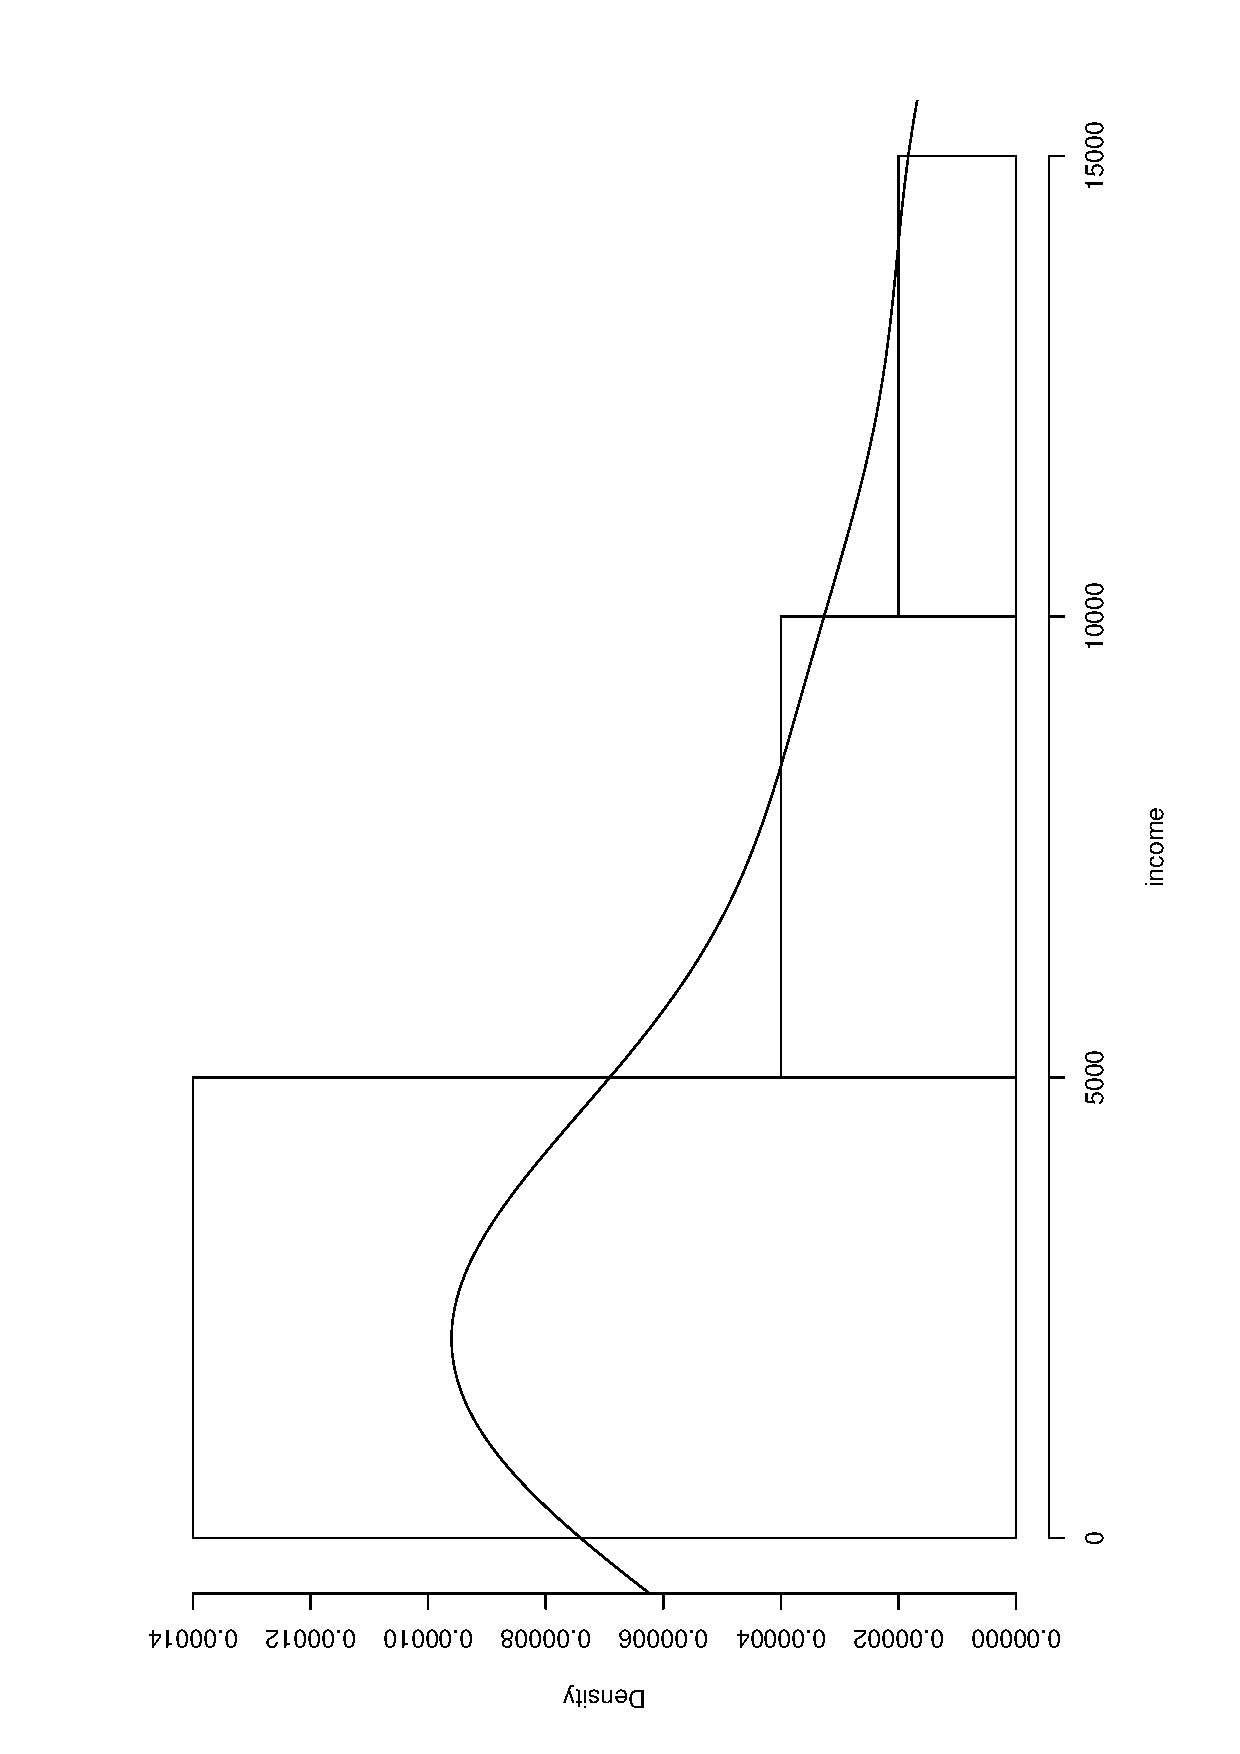
\includegraphics[scale=0.3, angle=90]{images/incomerhist.pdf}
%end{latexonly}
\htmlonly{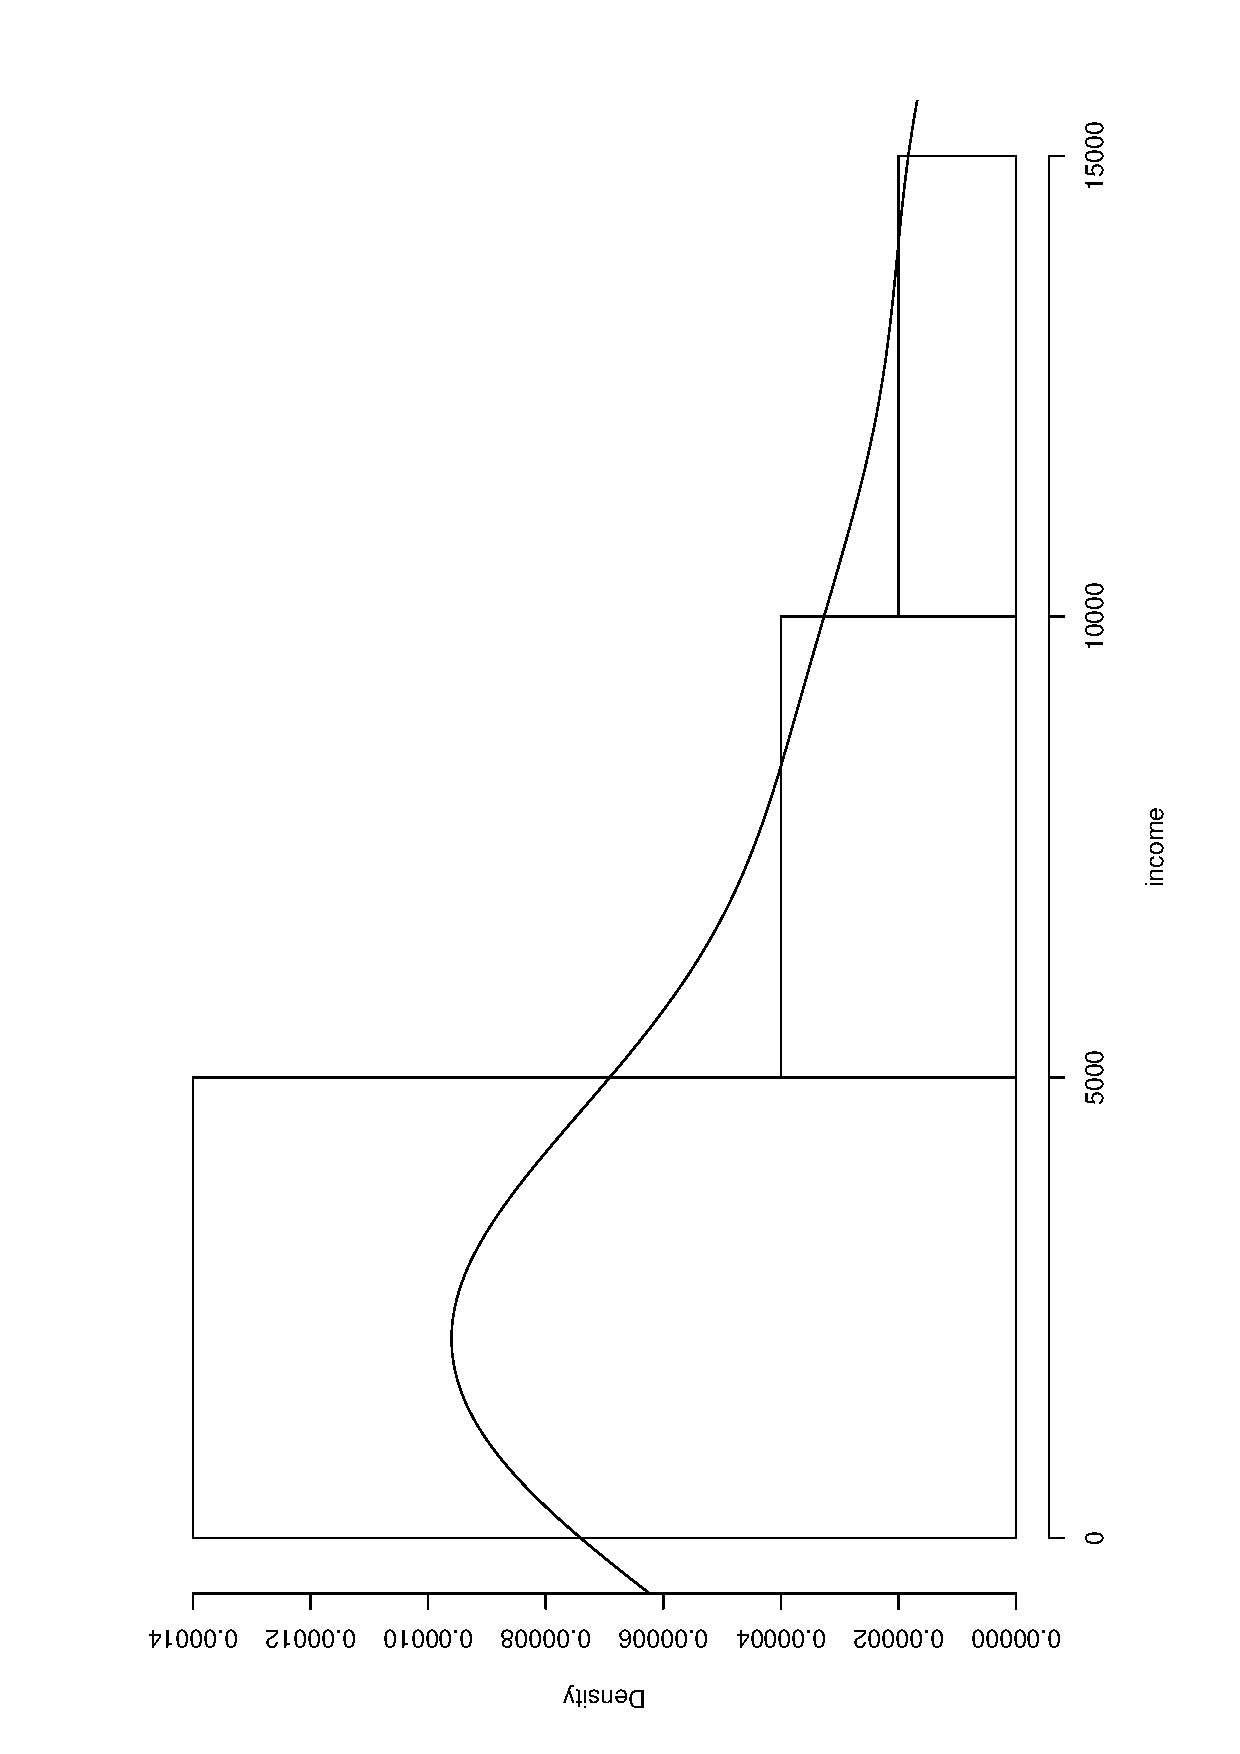
\includegraphics[scale=0.3, angle=90]{images/incomerhist.jpg}}
\end{center}

We can investigate a correlation \index{correlation} between attributes by plotting a scatter
plot (\module{rpy}\index{R}\index{rpy} library required):

\begin{verbatim}
>>> households.r_scatter("persons", "income")
\end{verbatim}
\begin{center}
%begin{latexonly}
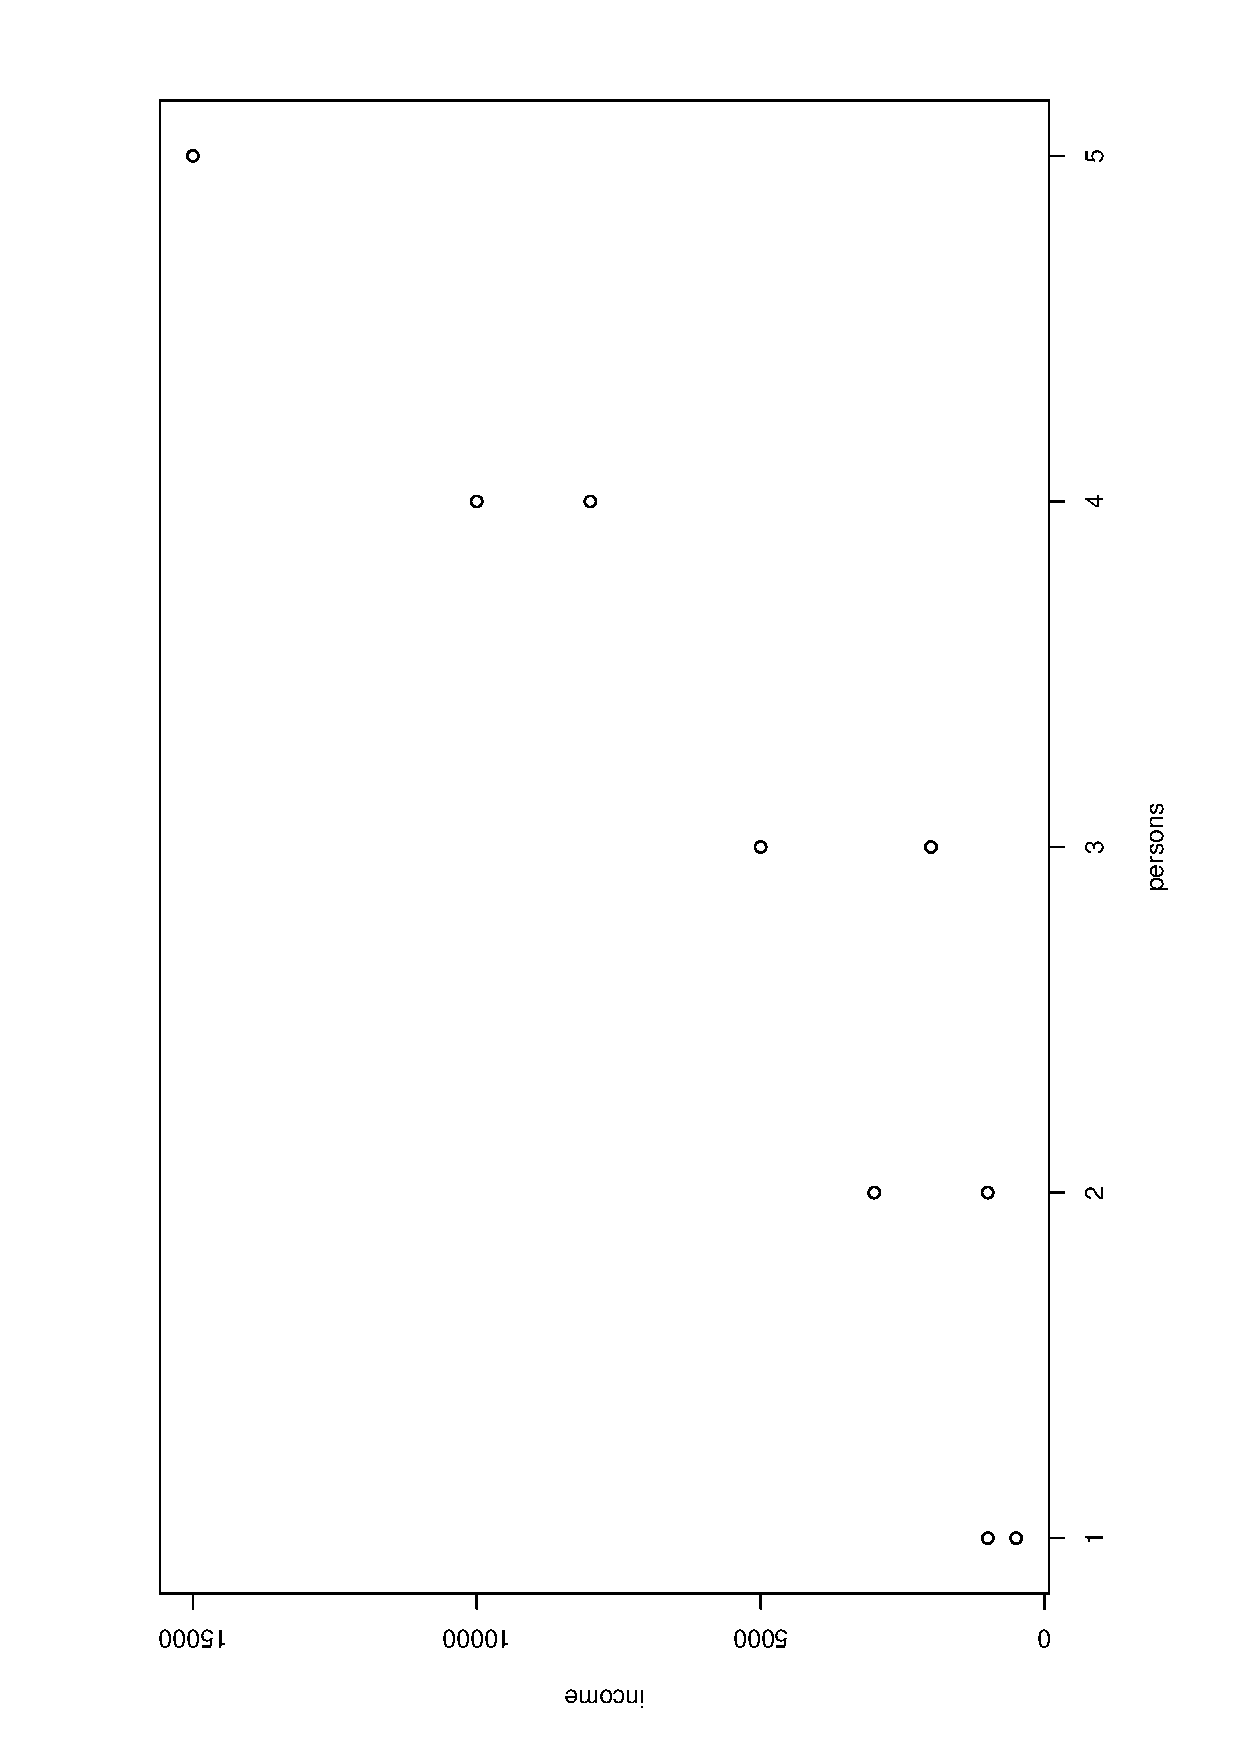
\includegraphics[scale=0.3, angle=90]{images/incomerscatter.pdf}
%end{latexonly}
\htmlonly{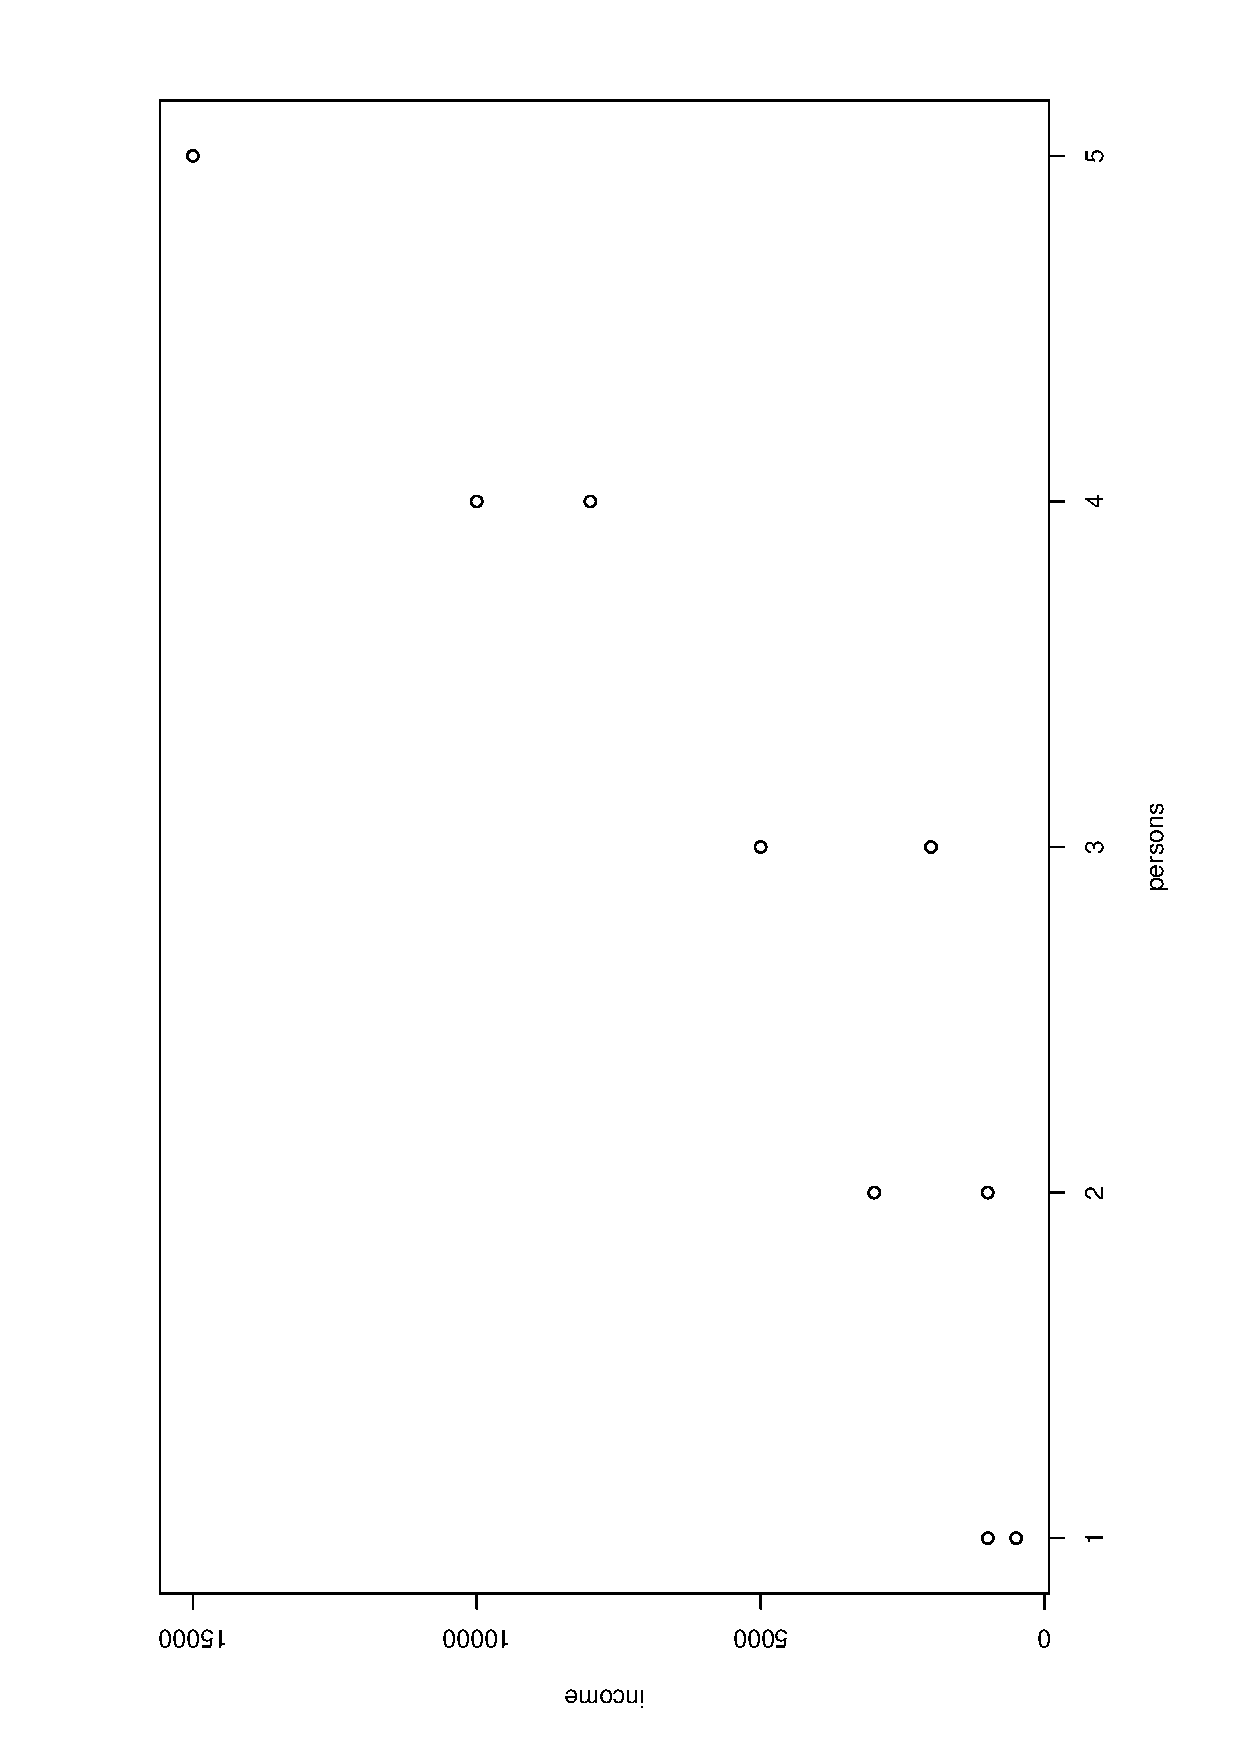
\includegraphics[scale=0.3, angle=90]{images/incomerscatter.jpg}}
\end{center}

\begin{verbatim}
Correlation coefficient:  0.919147133827
\end{verbatim}

The correlation coefficient between two attributes and the correlation matrix of several attributes, respectively,
can be obtained by:
\begin{verbatim}
>>> households.correlation_coefficient("persons", "income")
0.91914713382720947
>>> households.correlation_matrix(["persons", "income"])
array([[ 1.        ,  0.91914713],
       [ 0.91914713,  1.        ]], type=float32)
\end{verbatim}

A summary of data in a dataset can by given by:

\begin{verbatim}
>>> households.summary()
Attribute name        mean           sd           sum        min     max
-------------------------------------------------------------------------
       persons         2.7         1.34            27          1       5
        income      4850.0      4749.56         48500        500   15000
       


Size: 10  records
identifiers:
        household_id  in range  1 - 10
\end{verbatim}

To add an attribute to the set of households, for example each
household's location, we do
\begin{verbatim}
>>> households.add_primary_attribute(data=[4,6,9,2,4,8,2,1,3,2], name="location")
>>> households.get_attribute_names()
['household_id', 'persons', 'location', 'income']
\end{verbatim}
If the attribute "location" already exists in the dataset, the values are
overwritten.

To change specific values in a dataset, one can use


\begin{verbatim}
>>> households.modify_attribute(name="location", data=[0,0], index=[0,1])
>>> households.get_attribute("location")
array([0, 0, 9, 2, 4, 8, 2, 1, 3, 2])
\end{verbatim}
Here the argument \verb|index| determines the index of the data that are
modified.

To determine the location of household with \verb|household_id| $= 5$,
do
\begin{verbatim}
>>> households.get_data_element_by_id(5).location
4
\end{verbatim}

In order to store data in one of the supported formats,
you can use the {\tt storage} object created at the beginning of this section, or create a new one using
a different type of storage:

 
\begin{verbatim}
>>> households.write_dataset(out_storage=storage,
                             out_table_name="households_output")
\end{verbatim}

Each dataset 
  should have a unique dataset name that is used as an identification in
  variable computation (see
  Section~\ref{sec:variable-names}). 

\begin{verbatim}
>>> households.get_dataset_name()
'household'
\end{verbatim}

The \package{urbansim} package contains many pre-defined dataset classes, such as \class{HouseholdDataset}, \class{GridcellDataset},
  \class{JobDataset}, \class{ZoneDataset}, \class{FazDataset}, \class{NeighborhoodDataset}, \class{RaceDataset},
  \class{RateDataset}. Some datasets are described in  Section~\ref{sec:urbansim-datasets},
  Table~\ref{tab:urbansim-datasets}. They are all children of \class{Dataset} with pre-defined values
  for some arguments, such as \verb|id_name|, \verb|in_table_name| or \verb|dataset_name|. 

  

%
\section{Working with Models}
%
Generally, each model class has a method \method{run()} that runs a simulation and
(if applicable) a method \method{estimate()} that runs an estimation of the model.
Models are initiated by a constructor that sets class attributes common to
both methods.

%
\subsection{Choice Model}
%
The class \class{ChoiceModel} implemented in \package{opus_core} is initiated with a choice set
and a set of components specifying some of the model behavior. The model can
be estimated and run for a set of agents (see Section~\ref{sec:choice-model} for details).

%
\subsubsection{Initialization}
%
Suppose we would like to simulate a process of households deciding among 3
choices using the discrete choice model theory. The number of persons in each
household should influence their decisions. We will model this behavior by
multinomial logit using a system of utility functions:
$$
\begin{array}{rcrr}
v_1 & = &\beta_{01} & \\
v_2 & = &  & \beta_{12}x \\
v_3 & = & \beta_{03} & +  \beta_{13}x
\end{array}
$$
Here, $\beta_{01}$ and $\beta_{03}$ are alternative specific constants and $x$
is a household variable ``persons''.

The model is initialized by
\begin{verbatim}
>>> from opus_core.choice_model import ChoiceModel
>>> choicemodel = ChoiceModel(
                       choice_set=[1,2,3],
                       utilities = "opus_core.linear_utilities",
                       probabilities = "opus_core.mnl_probabilities",
                       choices = "opus_core.random_choices")
\end{verbatim}
Thus, the model is composed by external implementations of model steps, such
as computing utilities, computing probabilities and computing choices,
specified as \module{package.module_name}. Those modules must contain a
class of the same name and a method \method{run()} that performs the actual
computation (see Section~\ref{sec:choice-model} and Sections~\ref{sec:utilities}-\ref{sec:choices}
for more details).

%
\subsubsection{Estimation}
%
In order to estimate coefficients $\beta$ from the above equations, we define
a specification:


\begin{verbatim}
>>> from numpy import array
>>> from opus_core.equation_specification import EquationSpecification
>>> specification = EquationSpecification(
      coefficients = array([
        "beta01",      "beta12",         "beta03",    "beta13"
                          ]),
      variables = array([
        "constant","household.persons", "constant", "household.persons"
                        ]),
      equations = array([
           1,              2,                3,             3
                    ])
      )
\end{verbatim}
Each of the arguments is an array where the $i$th element describes the $i$th
coefficient in an equation determined by the $i$th element in the argument
\verb|equations|. For example, \verb|beta12| is a coefficient connected to the
household variable ``persons'' in equation 2, and \verb|beta03| is a constant
used in equation 3. The prefix ``household'' in the variable name specifies
the name of the dataset \verb|households|.
In other words, we are using here a dataset-qualified name of an attribute explained in
Section~\ref{sec:opus-core-attribute-names}.
An optional argument \verb|submodels| can extend the specification
to a model with multiple submodels. The \class{EquationSpecification} class is described
in Section~\ref{sec:specification} in more detail.

Our estimation data must include an attribute specifying choices that
households made:
\begin{verbatim}
>>> households.add_primary_attribute(data=[1,2,2,2,1,3,3,1,2,1], name="choice_id")
\end{verbatim}

The estimation is done by passing the specification, the agent set for
estimation and a name of the module that implements the actual estimation to
the method \method{estimate()}:

\begin{verbatim}
>>> coefficients, other_results = choicemodel.estimate(
                         specification, households, 
                         procedure="opus_core.bhhh_mnl_estimation")
\end{verbatim}
\begin{verbatim}
Estimating Choice Model (from opus_core.choice_model): started on 
                                                    Wed Nov  5 12:04:17 2008
    submodel: -2
    Convergence achieved.
    Akaike's Information Criterion (AIC):  26.142396805
    Number of Iterations:  144
    ***********************************************
    Log-likelihood is:            -9.07119840248
    Null Log-likelihood is:       -10.9861228867
    Likelihood ratio index:       0.174303938155
    Adj. likelihood ratio index:  -0.189791752496
    Number of observations:       10
    Suggested |t-value| >         1.51742712939
    Convergence statistic is:     0.000990037670084
    -----------------------------------------------
    Coeff_names	estimate	std err		t-values
        beta01	0.432678	 3.14438	0.137604
        beta03	-4.51824	 21.7087	-0.208131
        beta12	0.180115	 1.72541	 0.10439
        beta13	 1.34052	 4.18176	0.320564
    ***********************************************
    Elapsed time:  0.064521 seconds
Estimating Choice Model (from opus_core.choice_model): completed.........0.1 sec

\end{verbatim}
The estimation module given in the argument \verb|procedure| is a child of
\class{EstimationProcedure} (see Section~\ref{sec:estimation-procedure}), must
contain a method \method{run()} and should return a dictionary with keys
''estimators'' and ``standard_errors'' respectively, that contain arrays of
the estimated values and their standard errors, respectively.  The \method{estimate()}
method returns a tuple where the first element is an instance of
class \class{Coefficients} and the second element is a dictionary with all
results returned by the estimation \verb|procedure|.

A coefficient object can
be stored in a storage. For example, to store the computed coefficients as an
ASCII file \file{mycoef.tab} in the directory defined in the \verb|storage| object
on page~\pageref{storagepage}, do

\begin{verbatim}
>>> coefficients.write(out_storage=storage, out_table_name="mycoef")
\end{verbatim}
Again, other types of storage can be used here.

 %

\subsubsection{Simulation}
%
The coefficients that result from the estimation run can be directly plugged
into a simulation run:

\begin{verbatim}
>>> choices = choicemodel.run(specification,  coefficients, households)
Running Choice Model (from opus_core.choice_model): 
                                            started on Wed Nov  5 12:10:20 2008
    Total number of individuals: 10
    ChoiceM chunk 1 out of 1.: started on Wed Nov  5 12:10:20 2008
        Number of agents in this chunk: 10
    ChoiceM chunk 1 out of 1.: completed.................................0.0 sec
Running Choice Model (from opus_core.choice_model): completed............0.0 sec
>>> choices
array([1, 2, 1, 2, 2, 3, 3, 1, 2, 3])
\end{verbatim}
The resulting \verb|choices| is an array specifying the choice for each household. We can
now assign those values to the dataset: 
\begin{verbatim}
>>> households.modify_attribute(name="choice_id", data=choices)
\end{verbatim}

Note that multiple runs will produce different results, which is due to random
numbers \index{random numbers} used within the model. In order to receive reproducible results\index{reproducible results}, one
can fix the seed of the random number generator. The call above was
preceded by
\begin{verbatim}
>>> from numpy.random import seed
>>> seed(1)
\end{verbatim}

For demonstration purposes, we use the same dataset of households
for estimation and simulation. This would not be usually the case in real
simulation runs.

We can also create a coefficient class and assign their values directly
(see Section~\ref{sec:coefficients} for more details):

\begin{verbatim}
>>> from opus_core.coefficients import Coefficients
>>> coefficients = Coefficients(
                     names=array(["beta01", "beta12", "beta03", "beta13"]),
                     values=array([0.5,      0.2,       -5.0,     1.3]))
\end{verbatim}

If a variable $x$ in the utility equations is choice dependent,
one can create a dataset of choices and assign this attribute to the
dataset. Besides a list and an array, the argument \verb|choice_set| in the
\class{ChoiceModel} constructor also accepts a dataset. 

%
\subsection{Location Choice Model}
%
\label{sec:LCM}
%
The \class{LocationChoiceModel} class implemented in \package{urbansim} is a special case of the
\class{ChoiceModel} class (see Section~\ref{sec:location-choice-model} for details).
The choice set is a set of locations that agents choose
from. A set of locations can be sampled to each agent.

Suppose that in addition to the set of 10 households, we have a set of 9
locations with the attributes cost of living and capacity, respectively,
stored in a file \file{locations.tab}:
\begin{verbatim}
location  cost  capacity
1        500    1
2        200    1
3        600    2
4       1000    3
5        100    1
6       2000    3
7        300    1
8        400    1
9        800    2
\end{verbatim}
One can represent this dataset using again the  \class{Dataset} class:
\label{page:tutorial-gc-locations}
\begin{verbatim}
>>> locations = Dataset(in_storage = storage,
                        in_table_name = 'locations', 
                        id_name='location',
                        dataset_name='gridcell')
\end{verbatim}
We use here the \verb|storage| object
created on page~\pageref{storagepage}, since the table is stored in the same directory.

Suppose, we wish to simulate a process of agents choosing locations.  As a
first example, suppose our only predictor is the location attribute cost with
a coefficient value of $-0.01$ (modeling a negative effect of cost on the
choice preferences). (For simplicity, we skip the estimation process and
consider the coefficient value as given.) As in the previous section, we
create a coefficient object, a specification object and a choice model object,
respectively:


\begin{verbatim}
>>> coefficients = Coefficients(names=("costcoef", ), values=(-0.01,))
>>> specification = EquationSpecification(variables=("gridcell.cost", ),
                                          coefficients=("costcoef", ))
>>> from urbansim.models.household_location_choice_model import \
                               HouseholdLocationChoiceModel
>>> hlcm = HouseholdLocationChoiceModel(
                               location_set = locations,
                               sampler=None,
                               compute_capacity_flag=False)
\end{verbatim}
The household location choice model (HLCM) is a child of 
\class{LocationChoiceModel} with some useful default settings.  
The argument \verb|sampler| specifies a module to be
used for sampling locations to each agent. If it is None, all locations are
considered as a possible alternative for each agent.  The argument
\verb|compute_capacity_flag| specifies if the procedure should take capacity of
locations into account.

We can run the HLCM by using the method \method{run()}
which takes as obligatory arguments \verb|specification|, \verb|coefficients|
and the set of agents for which the model runs.  

\begin{verbatim}
>>> seed(1)
>>> result = hlcm.run(specification, coefficients, agent_set=households)
Running Household Location Choice Model 
                 (from urbansim.models.household_location_choice_model): 
                                     started on Wed Nov  5 12:53:11 2008
    Total number of individuals: 10
    HLCM chunk 1 out of 1.: started on Wed Nov  5 12:53:11 2008
        Number of agents in this chunk: 10
    HLCM chunk 1 out of 1.: completed....................................0.0 sec
Running Household Location Choice Model 
      (from urbansim.models.household_location_choice_model): completed...0.0 sec

\end{verbatim}

The results of the HLCM run determine locations that
agents have chosen. The model modifies values of the attribute `location' of
the agent set or adds this attribute to the dataset, if it doesn't exist:

\begin{verbatim}
>>> households.get_attribute("location")
array([5, 5, 5, 5, 5, 7, 7, 2, 5, 5])
\end{verbatim}

One way of visualizing results of the HLCM run is to plot a 
histogram{\index{histogram}\index{plotting!histogram}} of the
choices, including the capacity of each location (requires \module{matplotlib}
library):

\begin{verbatim}
>>> hlcm.plot_choice_histograms(capacity=locations.get_attribute("capacity"))
\end{verbatim}
\begin{center}
%begin{latexonly}
\includegraphics[scale=0.5, angle=0]{images/hlcmhist.pdf}
%end{latexonly}
\htmlonly{\includegraphics[scale=0.6, angle=0]{images/hlcmhist.jpg}}
\end{center}
In our case, more agents decided for the fifth and seventh location than there
are units available (which corresponds to the fact that those are two of the three cheapest locations).

In the above example, the discrete choice model consists of steps such as
computing utilities via the \class{opus_core.linear_utilities} class, computing
probabilities via the \class{opus_core.mnl_probabilities} class and computing
choices via the \class{opus_core.random_choices} class. These components
(default values) can be easily exchanged by other implementations. For
example, the class \class{urbansim.lottery_choices} for computing choices
takes into account capacity and forces agents to re-decide, if there is an
overflow in the locations capacity:
\begin{verbatim}
>>> number_of_agents = "gridcell.number_of_agents(household)"
>>> hlcm2 = HouseholdLocationChoiceModel(
                         location_set = locations,
                         sampler=None,
                         choices="urbansim.lottery_choices",
                         compute_capacity_flag=True,
                         capacity_string="capacity",
                         number_of_agents_string=number_of_agents,
                         number_of_units_string="capacity",
                         run_config={"lottery_max_iterations":10})
\end{verbatim}

The argument \verb|choices| is the full name of the module in which the choice
class is implemented. This module
must contain a class of the same name, i.e.
\class{lottery_choices} in this case, be a child of \package{opus_core} class \class{Choices}
(see Section~\ref{sec:choices}) and have a method \method{run()}.  Further arguments define the name of
the capacity attribute, name of the variable that computes number of agents in
each location (more about variable names in Section~\ref{sec:variable-names}), name of the
variable/attribute that determines the total number of units for each location. 
The argument \verb|run_config| is a dictionary that contains parameters for the simulation. In this example it contains a value
of how many times the households can re-decide if there is an overflow.

We run the above model:
\begin{verbatim}
>>> seed(1)
>>> result = hlcm2.run(specification, coefficients, households)
Running Household Location Choice Model 
                     (from urbansim.models.household_location_choice_model): 
                                            started on Wed Nov  5 18:18:58 2008
    Total number of individuals: 10
    HLCM chunk 1 out of 1.: started on Wed Nov  5 18:18:58 2008
        Number of agents in this chunk: 10
        Available capacity: 15.0 units.
        Number of unplaced agents: 0 (in 4 iterations)
    HLCM chunk 1 out of 1.: completed....................................0.0 sec
    gridcell.number_of_agents(household).................................0.0 sec
Running Household Location Choice Model 
     (from urbansim.models.household_location_choice_model): completed...0.0 sec
>>> hlcm2.plot_choice_histograms(capacity=locations.get_attribute("capacity"))
\end{verbatim}
\begin{center}
%begin{latexonly}
\includegraphics[scale=0.5, angle=0]{images/hlcm2hist.pdf}
%end{latexonly}
\htmlonly{\includegraphics[scale=0.6, angle=0]{images/hlcm2hist.jpg}}
\end{center}

\begin{verbatim}
>>> households.get_attribute("location")
array([9, 3, 9, 5, 4, 3, 7, 2, 8, 1])
\end{verbatim}
Now there is no overflow. Moreover, fourth and sixth locations still have free
units available, since they are the most expensive places. The agents were `forced'
to re-decide three times (i.e. 4 iterations in total). If the maximum
number of iterations given in \verb|run_config| would be reached without
placing all agents, the whole model would run automatically again. It would not be
very useful in this simple example, but the model is set-up for more complex situations,
including sampling of locations. Therefore in a new run, agents would sample
different locations which could solve the collision from the previous run.

Finally, agents that were not
placed have values smaller equal zero in the ``location'' attribute.

\package{urbansim} implements several location choice models.
Figure~\ref{fig:urbansim-model} in Section~\ref{sec:urbansim-models} shows
a hierarchical structure of the models.


%
\subsection{Regression Model}
%
\label{sec:RM}
%
Opus offers an infrastructure for estimation and simulation of a regression model
(see Section~\ref{sec:regression-model} for details).
Suppose our set of grid cells from the previous section has an attribute
``distance_to_cbd'' that contains information about the distance to the
central business district (cbd):

\begin{verbatim}
location cost  distance_to_cbd
1        500             5
2        200            10
3        600             5
4       1000             1
5        100            20
6       2000             0
7        300             7
8        400             7
9        800             3
\end{verbatim}

One can add the new attribute to the existing set of locations by:
\begin{verbatim}
>>> locations.add_primary_attribute(name="distance_to_cbd",
                                    data=[5,10,5,1,20,0,7,7,3])
\end{verbatim}

The cost of living in this dataset is highly correlated with
the distance to cbd and we can thus predict the cost using the regression model.

%
\subsubsection{Initialization}
%
The model is initialized by:
\begin{verbatim}
>>> from opus_core.regression_model import RegressionModel
>>> rm = RegressionModel(regression_procedure="opus_core.linear_regression")
\end{verbatim}
As in the case of choice model, the model is composed by model components, here
by plugging the appropriate regression procedure. The
regression procedure is a child of \class{Regression} (see Section~\ref{sec:regression}),
must have a method \method{run()} that gets as arguments a
multidimensional data array and a one-dimensional array of coefficients, and
returns a one-dimensional array of the regression outcome.

The \class{linear_regression} module implemented in \package{opus_core} is the default
procedure for the \class{RegressionModel} constructor and thus, it can be omitted.

%
\subsubsection{Estimation}
%
The specification for the above example consists of one variable and one
constant for the intercept:

\begin{verbatim}
>>> specification = EquationSpecification(
                          variables=array(["constant", "gridcell.distance_to_cbd"]),
                          coefficients=array(["constant", "dcbd_coef"]))
\end{verbatim}
The estimation for predicting the cost of living is run by:
\begin{verbatim}
>> coef, other_results = rm.estimate(specification, dataset=locations,
                              outcome_attribute="gridcell.cost",
                              procedure="opus_core.estimate_linear_regression")
Estimating Regression Model (from opus_core.regression_model):
                                            started on Mon Mar 19 21:14:33 2007
    Estimate regression for submodel -2
    Number of observations: 9
    R-Squared:             0.536420010196
    Adjusted R-Squared:    0.470194297367
    Suggested |t-value| >  1.48230380737
    -----------------------------------------------
    Coeff_names estimate        SE      t-values
      constant   1114.07         213.758         5.21183
     dcbd_coef  -71.1493         24.9995        -2.84603
    ===============================================

Estimating Regression Model (from opus_core.regression_model): completed...0.4 sec
\end{verbatim}
The estimation procedure that is passed as an argument is expected to be
a child of \class{EstimationProcedure} (see Section~\ref{sec:estimation-procedure}) and have a
method \method{run()} that takes as arguments a
multidimensional data array and an instance of a class specified by the
argument \verb|regression_procedure| in the model constructor. Thus, the
estimation procedure can use the same code that is used for simulation.

The resulting object of class \class{Coefficients} called \verb|coef| can be stored or
directly used for predicting cost of other locations.

\begin{verbatim}
>>> coef.summary()
Coefficient object:
size: 2
names: ['constant' 'dcbd_coef']
values:
[ 1114.07348633   -71.14933777]
standard errors:
[ 213.75848389   24.99952126]
t_statistic:
[ 5.211833   -2.84602809]
submodels: [-2 -2]
\end{verbatim}

%
\subsubsection{Simulation}
%
Suppose we have four locations with distance to cbd 2, 4, 6 and 8
respectively. We create a location dataset using
a storage type `dict'\index{Storage!dict}.
This type of storage is useful when we want to pass data directly without storing them on a physical storage media.

\begin{verbatim}
>>> dstorage = StorageFactory().get_storage('dict_storage')
>>> dstorage.write_table(table_name='gridcells',
                         table_data= {'id':array([1,2,3,4]),
                                      'distance_to_cbd':array([2,4,6,8])
                                    })
>>> ds = Dataset(in_storage=dstorage, in_table_name='gridcells',
                 id_name='id', dataset_name='gridcell')
\end{verbatim}
We have created a table in the RAM space called \file{gridcells} which is passed into the \class{Dataset} constructor.
Now we run the regression model with coefficients estimated in the previous
section:
 
\begin{verbatim}
>>> cost = rm.run(specification, coefficients=coef, dataset=ds)
Running Regression Model (from opus_core.regression_model):
                                        started on Mon Mar 19 21:35:23 2007
    Total number of individuals: 4
    RM chunk 1 out of 1.: started on Mon Mar 19 21:35:23 2007
        Number of agents in this chunk: 4
    RM chunk 1 out of 1.: completed......................................0.0 sec
Running Regression Model (from opus_core.regression_model): completed....0.0 sec
>>> cost
array([ 971.77478027,  829.47613525,  687.17749023,  544.87878418])
\end{verbatim}
As expected, the resulting cost decreases with increasing distance to cbd.

%
\section{Opus Variables} \index{Variables!Opus}
%
\label{sec:variables}
%
\subsection{Variable Concept}
%
\label{sec:variableconcept}
%


As mentioned in Section~\ref{sec:datasets}, a dataset has a set of
attributes\index{attributes}, such as income or persons, that are stored in a file or database.
We call such characteristics \emph{primary attributes}\index{primary attributes}\index{attributes!primary}.  
In addition, one is usually interested in attributes that are computed, for example using some
transformation of primary attributes.  We call those attributes \emph{variables}\index{variables},
or \emph{computed attributes}\index{attributes!computed}\index{computed attributes}.
They are simply handled as additional
``columns'' of a dataset to which they belong to, here denoted as
``parent dataset''.

In Opus, a variable is a class derived from the
\package{opus_core} class \class{Variable}.  Opus expressions 
(Chapter~\ref{chapter:expressions}),
as used in the expression library in the GUI and elsewhere, in fact just
are compiled into an automatically generated subclass of class \class{Variable}.
Section~\ref{sec:opus-variable} gives additional details about this class, 
including a discussion of how expressions are compiled.

In the GUI description, we used the expression library as a place to store and
reuse variable definitions.  We can also write expressions as Python strings
and use them from the command line.  The syntax of these expression language is 
that of Python, but the semantics
are somewhat different --- for example, a name like
\code{gridcell.distance_to_cbd} is a reference to the value of that
variable.  (If you just evaluated this in a Python shell you'd get an
error, saying that the \package{gridcell} package didn't have a
\code{distance_to_cbd} attribute.)  Further, expressions are evaluated lazily.
Here is a simple example:

\begin{verbatim}
>>> locations.compute_variables(["sqrt(gridcell.distance_to_cbd)"])
array([ 2.23606798,  3.16227766,  2.23606798,  1.        ,  4.47213595,
        0.        ,  2.64575131,  2.64575131,  1.73205081])
\end{verbatim}

The expressions are fed to the \method{compute_variables} method 
\index{compute_variables} of
\class{Dataset} (Section \ref{sec:compute-variables}), just as for simple
variable references.  (Given a new expression, Opus will compose a
new variable definition, including a \method{compute} and a
\method{dependencies} method, which computes the value of that expression.
It then saves the new variable definition in case the same expression is
encountered again --- see Section~\ref{sec:implementation-of-expressions}.
However, usually the user need not
be concerned about this.)  The \method{compute_variables} method evaluates
each variable (or expression) in turn, and returns the value of the last one.

For variables defined by hand as Python classes (rather than using Tekoa expressions), the
name of the class for a given variable is identical to the name of the module 
in which it is implemented.
The module is stored in a directory whose name corresponds to the name of
the parent dataset. Note that the variable 
name must be all lower case.

The variable class must have a method \method{compute()} 
that returns a numpy array of
variable values. The size of that array must correspond to the number of entries in the parent
dataset. The \method{compute()} method takes an argument called
\verb|dataset_pool| containing references to the appropriate set of datasets to
use for computing this variable. From the \method{compute()} method, the parent dataset can be
accessed  by \method{self.get_dataset()}.

If the variable depends on other attributes, they must be listed in the method
\method{dependencies()}, which returns a list of all dependent variables and
attributes in their fully-qualified names (see
Section~\ref{sec:opus-core-attribute-names} for details on attribute
specification).

As an example, consider a variable ``is_in_wetland'' for the gridcell dataset
\verb|locations| from Sections~\ref{sec:LCM} and~\ref{sec:RM}. The variable
returns \verb|True| for entries whose percentage of wetland is more than a certain
threshold, and \verb|False| otherwise. The module \file{is_in_wetland.py},
containing a class \class{is_in_wetland}, is stored in the directory
\file{gridcell} because
\begin{verbatim}
>>> locations.get_dataset_name()
'gridcell'
\end{verbatim}

The class is defined as follows:

\begin{verbatim}
from opus_core.variables.variable import Variable
class is_in_wetland(Variable):

    def dependencies(self):
        return ["gridcell.percent_wetland"]

    def compute(self, dataset_pool):
        return self.get_dataset().get_attribute("percent_wetland") > \
         dataset_pool.get_dataset('urbansim_constant')["percent_coverage_threshold"]

\end{verbatim}
The dependent attribute is a primary attribute and therefore specified as
a dataset-qualified name.  For our example, we populate the primary attribute:
\begin{verbatim}
>>> locations.add_primary_attribute(name="percent_wetland",
                                    data=[85,20,0,90,35,51,0,10,5])
\end{verbatim}

\begin{figure}[th]
\begin{verbatim}
from opus_core.variables.variable import Variable
from urbansim.functions import attribute_label
from variable_functions import my_attribute_label

class population(Variable):
    """Compute the total number of people residing in a gridcell, 
    by summing the attribute 'persons' over all households in the gridcell"""
    
    _return_type="int32"
    hh_persons = "persons"

    def dependencies(self):
        return [attribute_label("household", self.hh_persons), 
                attribute_label("household", "grid_id"), 
                my_attribute_label("grid_id")]

    def compute(self, dataset_pool):
        households = dataset_pool.get_dataset('household')
        return self.get_dataset().sum_dataset_over_ids(households, self.hh_persons)


from opus_core.tests import opus_unittest
from opus_core.tests.utils.variable_tester import VariableTester
from numpy import array
class Tests(opus_unittest.OpusTestCase):
    def test_my_inputs(self):
        gridcell_grid_id = array([1, 2, 3])
        #specify an array of 4 hh's, 1st hh's grid_id = 2 (it's in gridcell 2), etc.
        household_grid_id = array([2, 1, 3, 2]) 
        #specify how many people live in each household
        hh_persons = array([10, 5, 20, 30])

        tester = VariableTester(
            __file__,
            package_order=['urbansim'],
            test_data={
                "gridcell":{
                    "grid_id":gridcell_grid_id 
                    }, 
                "household":{ 
                    "household_id":array([1,2,3,4]),
                    "persons":hh_persons, 
                    "grid_id":household_grid_id
                }
            }
        )
        
        should_be = array([5, 40, 20])
        tester.test_is_close_for_family_variable(self, should_be)

if __name__=='__main__':
    opus_unittest.main()
\end{verbatim}
\caption{Definition of the `population' variable as a Python class}
\label{fig:population-variable}
\end{figure}

As another example, consider the \code{population} variable to compute
the population in each gridcell.  We refer
to a variable using a \verb#Pythonpath#, which provides a means for
Python to find modules and classes in a directory structure.  So, a
reference to this particular module using a \emph{fully qualified path}
would be \code{urbansim.gridcell.population}.  You can find all of the
existing variables by browsing on disk in the source code directory. 
The directory structure mirrors the parts of the variable name, so that
\code{urbansim.gridcell.population} is really pointing to
\file{opus/src/urbansim/gridcell/population.py}, which is also included 
in Figure~\ref{fig:population-variable} on page~\pageref{fig:population-variable}.

\subsubsection{Dataset Pool}
\index{dataset pool}
%
When computing variable values, Opus may need to access datasets used by
dependent variables, such as the \verb|urbansim_constant| dataset required by
\verb|is_in_wetland|, above.  These datasets are provided by the
\verb|dataset_pool| object passed into the variable's \method{compute} method.
This object is an instance of the \class{DatasetPool} class (see Section~\ref{sec:core-dataset-pool}).  It is responsible
for keeping a set of datasets for use when computing
variables.  If the requested dataset is in the pool already, it is returned
directly, otherwise it tries to find it in the given storage.

In order to find the appropriate dataset class for the requested dataset, the dataset
pool object searches the \file{datasets} directories of the Opus packages in
\verb|package_order|.  The first one to contain the appropriately named module
and class is used.  For instance, using the \verb|storage| object created on page~\pageref{storagepage},
for the definition:
\begin{verbatim}
>>> from opus_core.dataset_pool import DatasetPool
>>> dataset_pool = DatasetPool(package_order=['urbansim', 'opus_core'],
                               storage=storage)
\end{verbatim}
if \verb|dataset_pool| is asked for the ``household'' dataset, and does not
already have one in its pool, it will look in the \verb|storage|. In order to
create the corresponding dataset classes
it searches for a file
\file{household_dataset.py} (containing the class \class{HouseholdDataset}) first in \file{urbansim/datasets} and then in
\file{opus_core/datasets}. The first one found will be used.
\begin{verbatim}
>>> dataset_pool.datasets_in_pool()
{}
>>> hs = dataset_pool.get_dataset("household")
>>> dataset_pool.datasets_in_pool()
{'household': <urbansim.datasets.household_dataset.HouseholdDataset object
                                                               at 0x197c2f70>}
>>> hs.size()
10
\end{verbatim}
If the dataset pool is asked for \verb|urbansim_constant| and `urbansim' is included in \verb|package_order|,
it will use some \package{urbansim} specific constants defined in \file{urbansim/constants.py} (in addition to
user defined constants found on storage).

For the purpose of this example, we set the required constant by:
\begin{verbatim}
>>> constant = dataset_pool.get_dataset("urbansim_constant")
>>> constant["percent_coverage_threshold"] = 50
\end{verbatim}

\subsubsection{Invoking Computation}
\label{sec:compute-variables}
Computation of a variable is invoked using the \class{Dataset} method
\method{compute_variables()} passing the variable name in its fully-qualified
form and a dataset pool if other datasets are required for this variable:
 \label{page:compute-isnearcbd}

\begin{verbatim}
>>> locations.compute_variables("urbansim.gridcell.is_in_wetland",
                                  dataset_pool=dataset_pool)
urbansim.gridcell.is_in_wetland..........................................0.0 sec
array([ True, False, False,  True, False,  True, False, False, False], dtype=bool)
\end{verbatim}

The method returns the resulting values of the variable. The
\verb|compute_variables| method also accepts a list of variables to be
computed.  In this case it returns values of the last variable in the list.

 In addition, within the dataset, the variable can be accessed using its un-qualified name.
 Thus, the un-qualified names of variables including the primary
 attributes must be unique.
\begin{verbatim}
>>> locations.get_attribute("is_in_wetland")
array([ True, False, False,  True, False,  True, False, False, False], dtype=bool)
\end{verbatim}

\subsection{Interaction Variables}
\label{sec:interactions}

In order to work with variables that determine an
interaction between two datasets, there is a subclass of
\class{Dataset}, called
\class{InteractionDataset}. Attributes of this class are stored as
two-dimensional arrays (see Section~\ref{sec:interaction-set} for details).

To create an interaction set for households and gridcells from the previous
sections, do
\begin{verbatim}
>>> from opus_core.datasets.interaction_dataset import InteractionDataset
>>> interactions = InteractionDataset(dataset1 = households, dataset2 = locations)
\end{verbatim}
The dataset name is composed from dataset names of the two interacting datasets: 
\begin{verbatim}
>>> interactions.get_dataset_name()
'household_x_gridcell'
\end{verbatim}
Thus, an interaction variable for such dataset will be implemented in the
directory \file{household_x_gridcell}.

The \class{InteractionDataset} class contains several methods that are useful for
variable computation which must return a two-dimensional array. For example, a
variable defined as a multiplication of cost and income can be implemented as:

\begin{verbatim}
from opus_core.variables.variable import Variable

class cost_times_income(Variable):
    def dependencies(self):
        return ["gridcell.cost", "household.income"]

    def compute(self, dataset_pool):
        return self.get_dataset().multiply("income", "cost")
\end{verbatim}

This \class{cost_times_income} variable is mostly for illustration; it can
also be defined more conveniently as an expression (see Chapter~\ref{chapter:expressions}).

If we wish that only a subset of each dataset interact (for example for
memory reasons), we can pass the corresponding indices to the constructor:
\index{Memory!Loading a subset of a dataset}
\begin{verbatim}
>>> from numpy import arange
>>> interactions = InteractionDataset(dataset1 = households, dataset2 = locations,
                                  index1 = arange(5), index2 = arange(3))
\end{verbatim}
Here only the first 5 households and the first three gridcells interact.
The \method{compute()} method of the interaction variable should return an array of
size index1 $\times$ index2.


\begin{verbatim}
>>> interactions.compute_variables(
        ["urbansim.household_x_gridcell.cost_times_income"])
array([[  500000.,   200000.,   600000.],
       [ 1000000.,   400000.,  1200000.],
       [ 2500000.,  1000000.,  3000000.],
       [ 1500000.,   600000.,  1800000.],
       [  250000.,   100000.,   300000.]])
\end{verbatim}
\label{page:compute-interaction}

\package{urbansim} uses interaction variables mainly in \class{ChoiceModel} classes, where agents
interact with dataset of choices. The household location choice model object
\verb|hlcm| from Section~\ref{sec:LCM} can be for example estimated using two
variables, one of which is an interaction variable:

\begin{verbatim}
>>> specification = EquationSpecification(
                     variables=array([
                          "gridcell.cost",
                          "urbansim.household_x_gridcell.cost_times_income"]),
                     coefficients=array(["costcoef", "cti_coef"]))
>>> # place households
>>> households.add_primary_attribute(data=[2,8,3,1,5,4,9,7,3,6], name="location")
>>> coef, other_results = hlcm.estimate(specification, households)
Estimating Household Location Choice Model 
                     (from urbansim.models.household_location_choice_model): 
                                             started on Thu Nov  6 12:12:47 2008
    urbansim.household_x_gridcell.cost_times_income......................0.0 sec
    submodel: -2
    Convergence achieved.
    Akaike's Information Criterion (AIC):  39.8199022026
    Number of Iterations:  18
    ***********************************************
    Log-likelihood is:            -17.9099511013
    Null Log-likelihood is:       -21.9722457734
    Likelihood ratio index:       0.184882998032
    Adj. likelihood ratio index:  0.0938590753688
    Number of observations:       10
    Suggested |t-value| >         1.51742712939
    Convergence statistic is:     0.000302603242051
    -----------------------------------------------
    Coeff_names estimate        std err         t-values
      costcoef  -0.00312452     0.00339464      -0.920429
      cti_coef  4.45803e-07     5.34429e-07     0.834168
    ***********************************************
    Elapsed time:  0.02 seconds
Estimating Household Location Choice Model 
     (from urbansim.models.household_location_choice_model): completed...0.0 sec
\end{verbatim}

\label{page:iv-spec}

%
\subsection{Versioning}
\label{sec:versioning}
%
Opus uses a mechanism of versioning of variables and attributes. Each
variable/attribute  is initialized with a version number 0. Any subsequent
change of that variable/attribute  increments the version number. This allow us
to only recompute variables, if it is really needed. This means that if a
computation is invoked (by e.g.\ \verb|compute_variables()|), it is checked, if
any of the version numbers of all dependent variables has changed since the
last computation. The computation is performed only, if there was any change
in the dependencies tree. The mechanism is described in Section~\ref{sec:dependencies-tree}
in more detail.

For example,

\begin{verbatim}
>>> households.get_version("income")
0
>>> res = interactions.compute_variables([
             "urbansim.household_x_gridcell.cost_times_income"])
>>> interactions.get_version("cost_times_income")
0
>>> households.modify_attribute(name="income", data=[14000], index=[9])
>>> households.get_version("income")
1
>>> res = interactions.compute_variables([
             "urbansim.household_x_gridcell.cost_times_income"])
urbansim.household_x_gridcell.cost_times_income.......................0.0 sec
>>> interactions.get_version("cost_times_income")
1
\end{verbatim}

The first call of \method{compute_variables()} didn't perform the actual
computation, because nothing has changed since our previous computation on
page~\pageref{page:compute-interaction}.
After we modify one element of the ``income'' attribute
(note that ``income'' is a dependent variable of
``cost_times_income'' defined in the \method{dependencies()} method), the
variable is recomputed and the version number is increased.

\subsection{Using Arguments in Variable Names}
\label{sec:tutorial-numbersinvariables}

Opus offers the possibility of including a number or a character string into
variable name which is then passed to the variable constructor as an argument.
The module/class name of such variable corresponds to a pattern in which a
number is replaced by `DDD' and a string is replaced by `SSS'\@.  For example,
a similar variable to \class{is_in_wetland} in Section~\ref{sec:variableconcept} can be
implemented in a way that the threshold is directly included in the variable
name, such as \\
\class{is_in_wetland_if_threshold_is_80}. Here, we give an example of variable
of the type \verb|is_near_|{\em location}\verb|_if_threshold_is_|{\em number}.
As {\em location} we can use e.g. `highway',  `arterial', or `cbd'.
The class name is \class{is_near_SSS_if_threshold_is_DDD} and must have a
constructor implemented which takes a string and a number as arguments:

\begin{verbatim}
from opus_core.variables.variable import Variable

class is_near_SSS_if_threshold_is_DDD(Variable):
    def __init__(self, location, number):
        self.location = location
        self.number = number
        Variable.__init__(self)

    def dependencies(self):
        return ["gridcell.distance_to_" + self.location]

    def compute(self, dataset_pool):
        distance_to_location = self.get_dataset().get_attribute(
                                        "distance_to_" + self.location)
        return distance_to_location < self.number
\end{verbatim}
We can then invoke the computation for the `cbd' location and different
thresholds by changing the variable name:
\begin{verbatim}
>>> res = locations.compute_variables(
      map(lambda threshold:
       "urbansim.gridcell.is_near_cbd_if_threshold_is_%s" % threshold, [2,4,7]))
urbansim.gridcell.is_near_SSS_if_threshold_is_DDD...................0.0 sec
urbansim.gridcell.is_near_SSS_if_threshold_is_DDD...................0.0 sec
urbansim.gridcell.is_near_SSS_if_threshold_is_DDD...................0.0 sec
\end{verbatim}


\begin{verbatim}
>>> locations.get_attribute("is_near_cbd_if_threshold_is_2")
array([False, False, False,  True, False,  True, False, False, False], dtype=bool)
>>> locations.get_attribute("is_near_cbd_if_threshold_is_4")
array([False, False, False,  True, False,  True, False, False,  True], dtype=bool)
>>> locations.get_attribute("is_near_cbd_if_threshold_is_7")
array([ True, False,  True,  True, False,  True, False, False,  True], dtype=bool)
\end{verbatim}

If the dataset \verb|locations| would have an attribute
``distance_to_highway'', we
could use the same variable implementation for variables
\class{is_near_highway_if_threshold_is_...}.

The arguments of the constructor are passed in the same number and order as
they appear in the variable name. For example, if the name would contain only
one pattern, say DDD, the constructor would expect only one argument, namely
an integer. The method \method{dependencies()} is called from
\method{Variable.__init__()}, therefore any class attributes used in
\method{dependencies()} (such as \verb|self.location| in this case) must be set
before the call of \\
\method{Variable.__init__()}.

\emph{Note: Arguments for variable names will probably be replaced with a
  more standard syntax in the future, for example
  \class{is_near(feature='highway', threshhold=2)}.  However, we don't have
  a specific date yet for this change.  We will try to preserve backward
  compatibility.}

\subsection{Expression Names and Aliasing}
\label{sec:urbansim-tutorial-aliasing}
\index{aliasing}

The expression library includes a name field for each expression.  This is
used to bind the name to the corresponding expression.  When using such
expressions intermixed with Python code, another mechanism is needed to
give a name to an expression -- this is done with something much like an
assignment statement, for example:

\code{lnpop = ln(urbansim.gridcell.population)}

This is treated as an expression, which can occur in the list of
expressions given to \method{compute_variables} or in an \file{aliases.py}
file (see below).  The value of the new alias is returned as the value of
the expression if it's the last item on the list of variables and
expressions.

It is convenient, and often more efficient
(Section~\ref{sec:expression-equality}), to gather all the expressions and
aliases for a particular package and dataset into one place.  When using 
XML-based configurations, the expression library component of the XML configurations
supports this nicely.  In older parts of the code using dictionary-based
configurations, the optional
\file{aliases.py}\index{alias.py file} file supports this functionality instead.
This file should define a single variable \code{aliases} to be a list of expressions,
each of which should define an alias.  This file is then placed in the same
directory as variables for that package and dataset.  For example, to
define aliases relevant to \code{urbansim.gridcell}, put an
\file{aliases.py} file into the \file{urbansim.gridcell} directory.  These
aliases can then be referred to using the fully-qualified name of the
alias.  When finding a variable referenced by a fully-qualified name, the
system first searches the aliases file (if present), and then the variable
definitions in the appropriate directory.

As an example, the directory \code{opus_core.test_agent} contains one
variable definition, for the variable \code{income_times_2}.  (This
directory and variable are used for unit tests for \package{opus_core}.)
The file \file{aliases.py} in that same directory contains the following:

\begin{verbatim}
aliases = [
    'income_times_5 = 5*opus_core.test_agent.income',
    'income_times_10 = 5*opus_core.test_agent.income_times_2'
    ]
\end{verbatim}

The first alias refers to a primary attribute (\code{test_agent.income}),
and the second to the variable.  These aliases can then be referred to
using a fully-qualified name, in exactly the same way as a variable,
for example

\code{opus_core.test_agent.income_times_5}.  

See the unit tests in
\file{opus_core.variables.expression_tests.aliases_file} for examples of
using these aliases.

\subsection{Using Interaction Sets in Expressions}
\label{sec:urbansim-tutorial-interaction-sets}
\index{interaction sets}

If you access an attribute of a component of an interaction set in the
context of that interaction set, the result is converted into a 2-d array
and returned.  These 2-d arrays can then be multiplied, divided, compared,
and so forth, using the numpy functions and operators.  For example,
suppose we have an interaction set \file{household_x_gridcell}.  The
component \file{household} set has an attribute \verb|income| with values
\verb|[100, 200, 300]|.  (These numbers are just to explain the concepts
--- obviously they aren't realistic incomes.)  The \file{gridcell}
component has an attribute \verb|cost| with values \verb|[1000, 1200]|.
Then evaluating

\begin{verbatim}
household_x_gridcell.compute_variables('urbansim.household.income')
\end{verbatim}

will return a 2-d array

\begin{verbatim}
[ [100, 100],
  [200, 200],
  [300, 300] ]
\end{verbatim}

and

\begin{verbatim}
household_x_gridcell.compute_variables('urbansim.gridcell.cost')
\end{verbatim}

returns

\begin{verbatim}
[ [1000, 1200],
  [1000, 1200],
  [1000, 1200] ]
\end{verbatim}

Then
\begin{verbatim}
household_x_gridcell.compute_variables(
            'urbansim.gridcell.cost*urbansim.household.income')
\end{verbatim}

evaluates to
\begin{verbatim}
[ [100000, 120000],
  [200000, 240000],
  [300000, 360000] ]
\end{verbatim}

Both the arguments to the operation and the result can be used in more
complex expressions.  For example, if we wanted to give everyone
a \$5000 income boost, and also scale the result, this could be done using
\verb|(household.income+5000)*gridcell.cost * 1.2|.

As another example, the model specification from
page~\pageref{page:iv-spec} can be modified by using an expression for the
interaction and taking its log:

\begin{verbatim}
>>> specification = EquationSpecification(
      variables=("gridcell.cost",
         "ln(urbansim.gridcell.cost*urbansim.household.income)"),
      coefficients=("costcoef", "cti_coef"))
\end{verbatim}


\subsection{Using Aggregation and Disaggregation in Expressions}
\label{sec:urbansim-tutorial-aggregation}
\index{Variable!aggregation} \index{Variable!disaggregation}

The methods \class{aggregate} and \class{disaggregate} are used to
aggregate and disaggregate variable values over two or more datasets.  
\index{aggregate variable} \index{disaggregate variable} The \class{aggregate} method associates
information from one dataset to another along a many-to-one relationship, while
the \class{disaggregate} method does the same along a one-to-many relationship. Some
examples are:

\begin{itemize}
\item \code{zone.aggregate(gridcell.population)}

\item \code{zone.aggregate(2.5*gridcell.population)}

\item \code{zone.aggregate(urbansim.gridcell.population)}

\item \code{neighborhood.aggregate(gridcell.population, 
  intermediates=[zone,faz])}

\item \code{neighborhood.aggregate(gridcell.population, 
  intermediates=[zone, faz], function=mean)}

\item \code{zone.aggregate(gridcell.population, function=mean)}

\item \code{region.aggregate_all(zone.my_variable)}

\item \code{region.aggregate_all(zone.my_variable, function=mean)}

\item \code{faz.disaggregate(neighborhood.population)}

\item \code{gridcell.disaggregate(neighborhood.population, 
      intermediates=[zone, faz])}

\end{itemize}

The syntax and semantics for these is as follows.

\subsubsection{Aggregation}

Suppose we have three different geographical units: gridcells, zones and
neighborhoods.  We have information available on the gridcell level and
would like to aggregate this information for zones and neighborhoods. We
know the assignments of gridcells to zones and of zones to neighborhoods.

First, we place the data for three neighborhoods and five zones into a dict storage:\index{Storage!dict}
\begin{verbatim}
>>> dstorage = StorageFactory().get_storage('dict_storage')
>>> dstorage.write_table(table_name='neighborhoods',
                         table_data={"nbh_id":array([1,2,3])}
                         )
>>> dstorage.write_table(table_name='zones',
                         table_data={"zone_id":array([1,2,3,4,5]),
                                     "nbh_id": array([3,3,1,2,1])}
                         )
\end{verbatim}

Then, we create the corresponding datasets: 
\begin{verbatim}
>>> neighborhoods = Dataset(in_storage=dstorage, in_table_name='neighborhoods',
                            dataset_name="neighborhood", id_name="nbh_id")
>>> zones = Dataset(in_storage=dstorage, in_table_name='zones',
                    dataset_name="zone", id_name="zone_id")
\end{verbatim}
Note that \verb|zones| contain assignments to neighborhoods in the
attribute `nbh_id'.  For the gridcell set, consider the dataset 
\verb|locations| defined on page~\pageref{page:tutorial-gc-locations}. We
add assignments of those nine locations to the zones:

\begin{verbatim}
>>> locations.add_primary_attribute(name="zone_id", data=[3,5,2,2,1,1,3,5,3])
\end{verbatim}
Note that any assignment must be done by using an attribute of the same name
as the unique identifier of the dataset that the assignment is made to.

As the next step, we prepare a dataset pool \index{dataset pool} for the variable computation, since we are dealing with variables
that involve more than one dataset. To make things easy, we explicitly insert
our three datasets into the pool:
\begin{verbatim}
>>> dataset_pool = DatasetPool(package_order=['urbansim', 'opus_core'],
                               datasets_dict={'gridcell': locations,
                                              'zone': zones, 
                                              'neighborhood':neighborhoods})
\end{verbatim}
An aggregation over one geographical level for the \verb|locations|
attribute `capacity' can be done by:

\begin{verbatim}
>>> aggr_var = "aggregated_capacity = zone.aggregate(gridcell.capacity)"
>>> zones.compute_variables(aggr_var, dataset_pool=dataset_pool)
aggregated_capacity = zone.aggregate(gridcell.capacity)..................0.0 sec
array([ 4.,  5.,  4.,  0.,  2.])
\end{verbatim}
By default, the aggregation function applied to the aggregated data is the
`sum' function. This can be changed by passing the desired function as second
argument in the variable name:
\begin{verbatim}
>>> aggr_var = \
"zone.aggregate(urbansim.gridcell.is_near_cbd_if_threshold_is_2, function=maximum)"
>>> zones.compute_variables(aggr_var, dataset_pool=dataset_pool)
zone.aggregate(urbansim.gridcell.is_near_cbd_if_threshold_is_2, function=maximum):
                                                            completed...0.4 sec
array([ 1.,  1.,  0.,  0.,  0.])
\end{verbatim}

The \method{aggregate} method accepts the following aggregation functions:
sum, mean, variance, standard_deviation, minimum, maximum,
center_of_mass. These are functions of the scipy package
\module{ndimage}.

An aggregation over two or more levels of geography is done by passing a
third argument into the \class{aggregate} method. It is a list of dataset
  names over which it is aggregated, excluding datasets
  for the lowest and highest level. For example, aggregating
the gridcell attribute `capacity' for the neighborhood set
can be done by:
\begin{verbatim}
>>> aggr_var2 = \
   "neighborhood.aggregate(gridcell.capacity, function=sum, intermediates=[zone])"
>>> neighborhoods.compute_variables(aggr_var2, dataset_pool=dataset_pool)
neighborhood.aggregate(gridcell.capacity, function=sum, intermediates=[zone])
    zone.aggregate(gridcell.capacity,function=sum).......................0.0 sec
neighborhood.aggregate(gridcell.capacity, function=sum, intermediates=[zone]):
                                                            completed...0.3 sec
array([ 6.,  0.,  9.])
\end{verbatim}

\subsubsection{Disaggregation}

Disaggregation is done analogously. The \class{disaggregate} method takes
information from a coarse set of entities and allocates it to a finer set of
entities, in the manner of a one-to-many relationship. By default, the function
for allocating data is to simply replicate the data on the parent entity for
each inheriting entity. The method takes one required argument, an
attribute/variable
  name, and one optional argument, a list of
dataset names. Here we add an attribute
``is_cbd'' to the neighborhood set and distribute it across gridcells:

\begin{verbatim}
>>> neighborhoods.add_primary_attribute(name="is_cbd", data=[0,0,1])
>>> disaggr_var = \
       "is_cbd = gridcell.disaggregate(neighborhood.is_cbd, intermediates=[zone])"
>>> locations.compute_variables(disaggr_var, dataset_pool=dataset_pool)
is_cbd = gridcell.disaggregate(neighborhood.is_cbd, intermediates=[zone])
    zone.disaggregate(neighborhood.is_cbd).......................0.0 sec
is_cbd = gridcell.disaggregate(neighborhood.is_cbd, intermediates=[zone]):
                                                           completed...0.0 sec
array([0, 0, 1, 1, 1, 1, 0, 0, 0])

\end{verbatim}

Note that since we used the dataset-qualified name for
``is_cbd'' in the \method{disaggregate} method, the attribute must be a
primary attribute of \verb|neighborhoods|.  The
\method{aggregate} and \method{disaggregate} methods both must have the
dataset name of the dataset for which they are computed before the method
name, e.g.\ \code{gridcell.disaggregate}.

To aggregate over all members of one dataset, one can use the
built-in method \method{aggregate_all}. It must be used with a dataset
  that has one element which is the case of the
\package{opus_core} dataset \class{AlldataDataset}
implemented in the directory \file{datasets}. For example, the total
capacity for all gridcells can be determined by:

\begin{verbatim}
>>> from opus_core.datasets.alldata_dataset import AlldataDataset
>>> alldata = AlldataDataset()
>>> alldata.compute_variables(
        "total_capacity = alldata.aggregate_all(gridcell.capacity, function=sum)",
        dataset_pool=dataset_pool)
total_capacity = alldata.aggregate_all(gridcell.capacity, function=sum)....0.0 sec
array([ 15.])
\end{verbatim}
In addition to \method{sum}, the \class{aggregate_all} class accepts all
functions that are accepted by the \class{aggregate} class;
the default is \method{sum}.

If the attribute being aggregated or disaggregated is a simple variable, it
should be either dataset-qualified or fully-qualified, i.e.\ always
including the dataset name and optionally including the package name.  The
attribute being aggregated can also be an expression.  (In this case,
behind the scenes the system generates a new variable for that expression,
and then uses the new variable in the aggregation or disaggregation
operations.  However, this isn't visible to the user.)  The result of an
aggregation or disaggregation can also be used in more complex expressions,
e.g. \code{ln(2*aggregate(gridcell.population))}.

\subsection{Number of Agents}
\index{number_of_agents}

A common task in modeling is to determine a number of agents of one dataset
  that are assigned to another dataset. For this
purpose, Opus contains a built-in method \class{number_of_agents}, which
takes as an argument the name of the agent dataset. For
example, our household dataset is assigned to the following
locations:
\begin{verbatim}
>>> households.modify_attribute(name="location",
                              data=[2, 8, 3, 1, 5, 4, 9, 7, 3, 6])
\end{verbatim}
Then, the number of households in each location can be determined by:

\begin{verbatim}
>>> dataset_pool.add_datasets_if_not_included({'household': households})
>>> locations.compute_variables("gridcell.number_of_agents(household)",
                                dataset_pool=dataset_pool)
gridcell.number_of_agents(household).....................0.0 sec
array([ 1.,  1.,  2.,  1.,  1.,  1.,  1.,  1.,  1.])
\end{verbatim}
Note that we had to add the household dataset to the dataset pool \index{dataset pool}
in order to have it available in the computation process.

Similarly, the number of zones in neighborhoods is computed by

\begin{verbatim}
>>> neighborhoods.compute_variables("neighborhood.number_of_agents(zone)",
                                    dataset_pool=dataset_pool)
neighborhood.number_of_agents(zone)......................0.0 sec
array([ 2.,  1.,  2.])
\end{verbatim}

As in the case of \method{aggregate} and \method{disaggregate}, the
\method{number_of_agents} method must be preceded by the `owner' dataset
name, e.g. \verb|neighborhood.number_of_agents| for computing on the
\verb|neighborhood| dataset.


\section{Creating a New Model}
%
\label{sec:tut-creating-new-model}
In most cases, a model would perform some operations on datasets. Opus' only
requirements for model classes are:
\begin{enumerate}
\item Being a child class of the \package{opus_core} class \class{Model}, and
\item have a method \method{run()}.
\end{enumerate}
Optionally, it can have a class attribute \verb|model_name|.

Thus, the following code is a model:
\begin{verbatim}
>>> from opus_core.model import Model
>>> from opus_core.logger import logger
>>> class MyModel(Model):
        model_name = "my model"
        def run(self):
            logger.log_status("I'm running!")
            return
\end{verbatim}
Then
\begin{verbatim}
>>> MyModel().run()
Running my model (from __main__): started on Tue Mar 28 17:41:04 2006
    I'm running!
Running my model (from __main__): completed..............................0.0 sec
\end{verbatim}

Packages \package{opus_core} and \package{urbansim} implement several models that can be used
as parent classes when developing a new model. The whole model hierarchy is shown in
Figure~\ref{fig:urbansim-model} in Section~\ref{sec:urbansim-models}.
We give here an example of implementing a new chunk model, making use of the \package{opus_core}
class \class{ChunkModel} (see Section~\ref{sec:chunk-model}) which automatically
processes the model in several chunks.

Suppose we wish to generate a certain number $n$ of normally distributed random numbers\index{random numbers}
to each agent of a dataset. The mean and variance of the distributions are agent's specific and are
given by two existing attributes of the dataset. 
The model returns an array of the means of the generated numbers
for each dataset member. The number of the generated values $n$ is user defined and thus it will be
passed as an argument. Since we expect that both $n$ and the dataset size can be large, we choose
the \class{ChunkModel} as the parent class which provides flexibility in saving memory. For this model,
we only need to define the method \method{run_chunk()} containing the actual computation,
since the \method{run()} method is defined
in the parent class (see Section~\ref{sec:chunk-model} for its arguments).

The model can be coded as follows:

\begin{verbatim}
>>> from opus_core.chunk_model import ChunkModel
>>> from numpy import apply_along_axis
>>> from numpy.random import normal

>>> class MyChunkModel(ChunkModel):
        model_name = "my chunk model"
        def run_chunk(self, index, dataset, mean_attribute, variance_attribute, n=1):
            mean_values = dataset.get_attribute_by_index(mean_attribute, index)
            variance_values = dataset.get_attribute_by_index(variance_attribute, 
                                                              index)
            def draw_rn (mean_var, n):
                return normal(mean_var[0], mean_var[1], size=n)
            normal_values = apply_along_axis(draw_rn, 0, 
                                             (mean_values, variance_values), n)
            return normal_values.mean(axis=0)
\end{verbatim}
The first two arguments of \method{run_chunk()} are obligatory (determined by the parent class),
the remaining ones are application specific. \verb|index| is an index of members of \verb|dataset|
that are processed in that chunk. The parent class takes care of ``chopping'' the dataset 
into appropriate chunks. \verb|mean_attribute| and \verb|variance_attribute| are names of the
\verb|dataset| attributes that determine the means and variances, respectively. The model extracts
the means and variances for dataset members of this chunk, generates a matrix of normally distributed
random numbers of size $n \times$ {\em number of agents in the chunk}, and returns the means for each agent.


In order to use this model, we need to create a dataset with the two required attributes for means and variances.
In our case, we have a dataset of $100,000$ entries. The mean and variance for the first half of the entries
is $0$ and $1$, respectively. The mean and variance for the second half of the entries
is $10$ and $5$, respectively.

\begin{verbatim}
>>> from numpy import arange, array
>>> from opus_core.storage_factory import StorageFactory
>>> storage = StorageFactory().get_storage('dict_storage')
>>> storage.write_table(table_name='dataset',
                        table_data={'id':arange(100000)+1,
                                    'means':array(50000*[0]+50000*[10]),
                                    'variances':array(50000*[1]+50000*[5])
                                    }
                        )
>>> from opus_core.datasets.dataset import Dataset
>>> mydataset = Dataset(in_storage=storage, in_table_name='dataset',
                        id_name='id', dataset_name='mydataset')
\end{verbatim}

Invoking a run of this model in five chunks is done by

\begin{verbatim}
>>> from numpy.random import seed
>>> seed(1)
>>> results = MyChunkModel().run(chunk_specification={'nchunks':5},
                                 dataset=mydataset,
                                 mean_attribute="means",
                                 variance_attribute="variances", n=10)
Running my chunk model (from __main__): started on Wed Mar 21 12:00:53 2007
    Total number of individuals: 100000
    ChunkM chunk 1 out of 5.: started on Wed Mar 21 12:00:53 2007
        Number of agents in this chunk: 20000
    ChunkM chunk 1 out of 5.: completed..................................0.7 sec
    ChunkM chunk 2 out of 5.: started on Wed Mar 21 12:00:54 2007
        Number of agents in this chunk: 20000
    ChunkM chunk 2 out of 5.: completed..................................0.7 sec
    ChunkM chunk 3 out of 5.: started on Wed Mar 21 12:00:54 2007
        Number of agents in this chunk: 20000
    ChunkM chunk 3 out of 5.: completed..................................0.7 sec
    ChunkM chunk 4 out of 5.: started on Wed Mar 21 12:00:55 2007
        Number of agents in this chunk: 20000
    ChunkM chunk 4 out of 5.: completed..................................0.7 sec
    ChunkM chunk 5 out of 5.: started on Wed Mar 21 12:00:56 2007
        Number of agents in this chunk: 20000
    ChunkM chunk 5 out of 5.: completed..................................0.7 sec
Running my chunk model (from __main__): completed........................3.7 sec
\end{verbatim}
The \method{run()} method expects the first two arguments, the remaining ones are optional
from the parent point of view. The first argument specifies the number of chunks (see
Section~\ref{sec:chunk-model}). By playing with different values for \verb|nchunks| and
\verb|n| one can see how quickly one can run out of memory. \index{Memory management!Using
multiple chunks per model}

Check the results, e.g. by checking the means of the two halves:
\begin{verbatim}
>>> results[0:50000].mean()
0.0010989375305175781
>>> results[50000:].mean()
10.000937499999999
\end{verbatim}

\section{Troubleshooting Python}
\label{sec:troubleshooting-python}

If you are unfamiliar with Python, here are some guidelines.

\begin{itemize}
  \item In Python, \verb|(|, \verb|{|, and \verb|[| each have different
  meanings.  Be careful to use the correct type of ``parentheses''.
  \item Be careful about whether the name has a single underscore, e.g.
  \verb|_one|, versus two leading underscores, e.g. \verb|__two|.  These can
  look similar in our documentation, so look carefully.
  \item In Python, words that have two double-underscores before and after the
  word, e.g. \verb|__init__| or \verb|__path__|, generally denote ``special''
  symbols.
  \item A command can be split over multiple lines. Normally, the Python continuation symbol `$\backslash$'
  at the end of each non-finished line is required. There is one exception:
  expressions in parentheses, straight brackets, or curly braces do not need '$\backslash$'.
  \item Indentation matters in Python. Code blocks (except with expressions
    in parentheses, straight brackets, or curly braces) are defined by
    their indentation.  We recommend only using spaces and not tabs, since
    combining them can be quite confusing if different systems display the
    tabs using different numbers of spaces.
\end{itemize}

% LocalWords:  borning urbansim PYTHONPATH AllTests HouseholdDataset mysql xml sql
% LocalWords:  mydatabase Dataset numpy matplotlib rpy ScenarioDatabase JobDataset
% LocalWords:  GridcellDataset ZoneDataset FazDataset NeighborhoodDataset RaceDataset RateDataset logit
% LocalWords:  numpy ChoiceModel rcrr submodels mycoef LocationChoiceModel
% LocalWords:  HLCM AgentLocationChoiceModel gridcells debuglevel config LCMs
% LocalWords:  UrbanSim EmploymentHomeBasedLocationChoiceModelCreator cbd coef
% LocalWords:  EmploymentIndustrialLocationChoiceModelCreator RegressionModel
% LocalWords:  EmploymentCommercialLocationChoiceModelCreator gridcell py un ln
% LocalWords:  DevelopmentProjectLocationChoiceModel InteractionDataset indices DDD
% LocalWords:  DevelopmentProjectCommercialLocationChoiceModelCreator hlcm init
% LocalWords:  DevelopmentProjectIndustrialLocationChoiceModelCreator powDDD th
% LocalWords:  DevelopmentProjectResidentialLocationChoiceModelCreator IDE cvs
% LocalWords:  Versioning versioning dataset datasets MySQL OpusDatabase pre nd

%%% Local Variables:
%%% mode: latex
%%% TeX-master: "userguide"
%%% End:
% LocalWords:  multinomial tuple EquationSpecification EstimationProcedure mnl
% LocalWords:  numpy LandPriceModel ResidentialLandShareModel variable's unary
% LocalWords:  DatasetPool threshhold sqrt elementwise lnpop disaggregate nbh
% LocalWords:  AlldataDataset ChunkModel nchunks

%% $Id: opus-core.tex,v 1.96 2007/06/01 23:49:22 borning Exp $

% Copyright (c) 2005-2007 Center for Urban Simulation and Policy Analysis,
% University of Washington.  Permission is granted to copy, distribute and/or
% modify this document under the terms of the GNU Free Documentation License,
% Version 1.2 or any later version published by the Free Software Foundation;
% with no Invariant Sections, no Front-Cover Texts, and no Back-Cover Texts.
% A copy of the license is included in the section entitled "GNU Free
% Documentation License".

\chapter{The \package{opus_core} Opus Package}

\emph{This section should walk through the Opus architecture, how it is
organized into packages, and where those are located on the file system.
Discuss where users should put their own scripts and data, and how they get
access to them.}

\section{Structure}

Opus is organized as a set of ``Opus packages''.  Each Opus package
encapsulates a set of functionality in a structure defined by a set of
required directories and files.  Opus will have simple mechanisms to create a
new package, bundle a package for distribution, and install or uninstall a
package. This chapter describes functionality provided by the Opus
package called \package{opus_core}.


\section{Datasets}
\label{sec:opus-core-datasets}

The basic class for dealing with data is called \class{Dataset},
\datasetindex implemented in
\verb|opus_core.datasets.dataset|. \datasetindex

A dataset \datasetindex is a collection of attributes \attributesindex for a particular type of entity,
such as a set of grid cells, or a set of households.  Each member in this set
has the same set of characteristics, such as income of households.  In Opus,
these characteristics are called attributes. \attributesindex

Conceptually, a dataset \datasetindex is similar to a table.  Each attribute \attributesindex is a column.
Each row describes the attribute values for one member of the dataset. \datasetindex

Some attributes \attributesindex are read from a data store, we call them {\it primary
  attributes}. \primaryattributesindex  Others, {\it computed attributes}, \computedattributesindex are computed by Opus
variable definitions.  Attributes \attributesindex can be also modified or created by models.


\subsection{Initialization}
%
The \class{Dataset} \datasetindex class is initialized by the following arguments:
\begin{description}
\item[resources] \index{resources} - on object of class \class{Resources}\index{Resources} (dictionary). It can
  contain any of the remaining arguments, but if an argument of the
  constructor is not None, it has a priority over the entry in
  \verb|resources|.
\item[in_storage] \index{in_storage} - an object of class \class{Storage}\index{Storage} for reading the data
  from (see Section~\ref{sec:data-storage}).
\item[id_name] \index{in_name} - a list of character strings giving the names of the unique
  identifiers of the dataset. \datasetindex If it is an empty list, a ``hidden'' identifier\index{hidden identifier}
  will be created, i.e. an additional attribute of the dataset that enumerates the entries.
\item[dataset_name] \index{database_name} - a character string giving the name of the dataset. \datasetindex
\item[out_storage] \index{out_storage} - an object of class \class{Storage}\index{Storage} for writing the data
  into (see Section~\ref{sec:data-storage}). This argument can be omitted in
  the constructor and instead directly passed to the
  \method{write_dataset()} method, which is the only method of the class that uses this argument.
\item[in_table_name] \index{in_table_name} - name of the table, directory or file that contains the
  data for this dataset \datasetindex (see Section~\ref{sec:data-storage} for the different
  meanings of this argument in the different storage classes).  This name also is the
  name used for this dataset \datasetindex in the cache (see below).
\item[out_table_name] \index{out_table_name} - name of the table, directory or file that the dataset \datasetindex
  should be written into (see Section~\ref{sec:data-storage} for the different
  meanings of this argument in the different storage classes). This argument
  can be omitted in the constructor and instead directly passed to the
  \method{write_dataset()} method.
\end{description}

All arguments are merged with \verb|resources| and kept in the class attribute \attributesindex
\verb|resources|.

The constructor determines all attributes \attributesindex available on the input storage
(primary attributes), \primaryattributesindex without loading them into memory. If \verb|id_name|
is an empty list, it loads at least one attribute \attributesindex from the storage in order to
obtain the dataset \datasetindex size. The constructor also sets up a reference to the
singleton \class{AttributeCache} which is used for caching data (see below).

%
\subsection{Loading Attributes}
\index{Memory!Lazy loading of attributes}
%
Primary attributes \primaryattributesindex are read lazily, i.e.\ they are loaded from the input
storage as they are needed, for example when they are required by a model or
by a variable definition. The loading can be also explicitly invoked by the
method \method{load_dataset()} \datasetindex which by default loads all attributes \attributesindex found on
the data storage. An optional argument \verb|attributes| \attributesindex can be passed which
is a list of attributes \attributesindex to be loaded.

Alternatively, the method \method{get_attribute(name)} \attributesindex invokes the specified
attribute \attributesindex to be loaded into memory if it has not been done before and returns
an array of values for this attribute. \attributesindex Note that when using a slow storage,
such as MySQL, loading several attributes \attributesindex at once using \method{load_dataset()} \datasetindex
(as opposed to one by one using \method{get_attribute()}) \attributesindex might be more
time efficient. \index{Memory management!Using multiple chunks per model}

Loaded or computed dataset \datasetindex attributes \attributesindex can be flushed into a simulation cache to
save memory \index{Memory!Flushing attributes} (using method
\method{flush_attribute(name)} \attributesindex for a specific attribute \attributesindex or
\method{flush_dataset()} for the whole dataset). \datasetindex Opus uses an FLT storage for
the simulation cache (see Section~\ref{sec:flt-storage}) which deals with
reading and writing data in a very efficient way. Thus, when using a slow
storage, it might be of an advantage to load the whole dataset \datasetindex at the beginning
of the dataset \datasetindex usage and flush all attributes. \attributesindex Then any subsequent load will be
performed on the fast cache.

\subsection{Computing Variables}
%
Datasets \datasetindex automatically compute each variable \variablesindex when, and only when,
needed. \index{Lazy evaluation}  This mechanism uses the dependency information
from each variable \variablesindex which gives an information about what variables \variablesindex this
variable \variablesindex depends on. Additionally, it is checked if variable's \variablesindex dependent
variables \variablesindex have changed (versioning mechanism).  The computation is invoked by
the dataset \datasetindex method \method{compute_variables()} which computes each of the
given variables \variablesindex if either (a) this variable \variablesindex has not been computed before, or
(b) the inputs to this variable \variablesindex (the values of variables \variablesindex upon which this
variable \variablesindex depends) have changed since the last computation.  Thus, invoking
\method{compute_variables()} \variablesindex on a single variable \variablesindex may either result in no more
computation, or have a ripple effect of computing many variables \variablesindex upon which
this one variable \variablesindex depends.  Lazily computing variables \variablesindex both helps minimize the
computational load as well as eliminating the need to worry about when
variables \variablesindex are computed: it will happen when, and only when, it is needed.

The method \method{compute_variables()} \variablesindex takes as an arguments a list of
variable \variablesindex names to be computed and an object of class \class{Resources} which
is a dictionary with all objects and arguments the variable \variablesindex (and its dependent
variables) \variablesindex need for the computation.

As mentioned before, datasets \datasetindex automatically load each attribute \attributesindex into memory
when, and only when, the data for that attribute \attributesindex is needed.  This is done
either as a side-effect of the \method{compute_variables()}, \variablesindex or via
\method{get_attribute()}. \attributesindex If the attribute \attributesindex is defined by a variable, \variablesindex you must
first use the \method{compute_variables()} \variablesindex method to force that variable \variablesindex to
compute its values for every member of the dataset. \datasetindex

\subsection{Attribute Names}
\label{sec:opus-core-attribute-names}
%
Attributes \attributesindex for a dataset \datasetindex can be specified in following ways:

\begin{description}
\item[Un-qualified name] (e.g.\ \code{population}) It is a character string
  without any dots or parentheses. It may contain numbers. Un-qualified
  names within a dataset \datasetindex must be unique. This way of
  specifying attributes \attributesindex may be used only for accessing
  already existing attributes \attributesindex within a dataset,
  \datasetindex e.g.  in the method
  \verb|get_attribute()|. \attributesindex

\item[Dataset-qualified name] (e.g.\ \code{gridcell.population}) Specifies
  a primary attribute \attributesindex of a specific dataset. \datasetindex
  It consists of a dataset \datasetindex name (e.g.  \verb|gridcell|) and
  an un-qualified attribute \attributesindex name (e.g.
  \verb|population|).  The dataset \datasetindex name allows you to
  disambiguate attributes \attributesindex of the same name in different
  datasets, \datasetindex when using outside of a dataset, \datasetindex
  e.g. in a model specification or in variable \variablesindex
  dependencies.

\item[Fully-qualified name] (e.g.\ \code{urbansim.gridcell.population})
  Specifies an Opus variable. \variablesindex It is the full name of the
  module or class in which the variable \variablesindex is defined. See
  Section~\ref{sec:variable-names} below, for more information.

\item[Expression] (e.g.\ \code{ln(urbansim.gridcell.population+1)})
  \index{expressions}
  Expressions are composed from variable names, constants, functions, and
  operators --- see Sections \ref{sec:urbansim-tutorial-expressions} and
  \ref{sec:opus-core-expressions}.

\end{description}
Each specification can be give an alias using the syntax
\verb|alias = expr|.  In that case, the alias name is used as un-qualified
name for this attribute and thus, values of this attribute can be accessed
by \verb|get_attribute(alias)|.

Opus contains a class \class{VariableName} \variablesindex that is initialized by passing a
name in one of the forms above. Instances of this class can be also used when
accessing attributes \attributesindex or invoking variable \variablesindex computation.

\subsection{Attribute Box}
\label{sec:attribute-box}
%
For each attribute \attributesindex that is loaded into memory or computed, the dataset \datasetindex creates
an instance of \class{AttributeBox}. \attributesindex This object holds all information
about the attribute, \attributesindex such as the data, attribute \attributesindex name (as \class{VariableName} \variablesindex
object), version, type, if it is cached or in memory, and a corresponding
instance of class \class{Variable} \variablesindex if this attribute \attributesindex is a variable. \variablesindex This
information can be accessed by the \class{AttributeBox} \attributesindex methods
\method{get_data()}, \method{get_variable_name()}, \variablesindex \method{get_version()},
\method{get_type()}, \method{is_cached()}, \method{is_in_memory()},
\method{get_variable_instance()}. \variablesindex The attribute \attributesindex box for a particular attribute \attributesindex
can be accessed by the dataset \datasetindex method
\method{_get_attribute_box(attribute_name)}, \attributesindex where the \verb|attribute_name| \attributesindex is
given in one of the  forms above.


\subsection{Visualizing Datasets}
%
Opus offers a few methods for plotting values of a dataset. \datasetindex They usually
require specific libraries to be installed, such as matplotlib (see your
Installation directions at your \file{opus_docs/docs/install.html}).

\subsubsection{One-dimensional Plots}
%
Attributes \attributesindex in a dataset \datasetindex are stored as one-dimensional arrays, thus they can be
plotted for example as a histogram \histogramindex or as a scatter plot. \scatterplotindex

\begin{description}
\item[\method{plot_histogram(name, ...)}] \histogramindex creates a histogram \histogramindex of attribute \attributesindex
\verb|name| using matplotlib. \matplotlibindex
\item[\method{r_histogram(name, ...)}] \rindex\histogramindex creates
such histogram \histogramindex including a density line using the rpy \rpyindex library.
\item[\method{r_scatter(name_x, name_y, ...)}] \rindex\scatterplotindex creates a scatter plot \scatterplotindex for two
attributes \attributesindex using the rpy \rpyindex library.
\end{description}

\subsubsection{Two-dimensional Plots}
%
One often is interested in a spatial graphical presentation of a dataset
attribute.  By default, datasets have no spatial coordinate axes.  If you want
a dataset to have a coordinate system, set the dataset's class variable
\verb|_coordinate_system| to be a tuple of the attribute names for the x and y
coordinates, e.g. to \verb|('relative_x','relative_y')|.  This information then
will be used by routines that need it.

\begin{description}
\item[\method{plot_map(name, ...)}] creates an image using the matplotlib \matplotlibindex
library.
\item[\method{r_image(name, ...)}] \rindex does the same using the rpy \rpyindex
library.
\item[\method{openev_plot(name, ...)}] \openevindex uses OpenEV \openevindex for creating the
  image.
\end{description}

\subsection{Subsets of Dataset}
\datasetindex\datasetsubsetindex
%
Opus implements a child class of \class{Dataset}, \datasetindex called \class{DatasetSubset}, \datasetsubsetindex
which allows to define a subset of a dataset. \datasetindex\datasetsubsetindex Conceptually, it is a viewing
window for the parent \class{Dataset} \datasetindex object, not a copy. Thus, any change in
the parent object is seen by the child.

It is initialized by passing the parent object and an index to the
constructor.  The index determines indices of elements within the parent
object that should be seen. Any call of \method{get_attribute()} \attributesindex returns
values corresponding to the index.

\subsection{Interaction Sets}
\label{sec:interaction-set}
%
Opus allows the programmer to create a dataset representing
the interaction between two other datasets, \datasetindex by using the class
\class{InteractionDataset}, which is a child of \class{Dataset}. \datasetindex It serves mainly
to enable the use of the Opus variable \variablesindex concept for variables \variablesindex
that are defined as an interaction between datasets as well, \datasetindex and thus are of a 2-d
shape. The class does not support loading from and writing to a storage.

\subsubsection{Initialization}
The class is initialized by the following arguments:
\begin{description}
\item[resources] - the same function as in \class{Dataset}. \datasetindex
\item[dataset1] - an instance of \class{Dataset}. \datasetindex
\item[dataset2] - an instance of \class{Dataset}. \datasetindex
\item[index1] - indices of \verb|dataset1| over which the interaction is
  done. If it is not given, all elements are taken.
\item[index2] - indices of \verb|dataset2| over which the interaction is
  done. If it is not given, all elements are taken.
\item[dataset_name] - a name of the interaction set. Default value is the
  dataset \datasetindex name of  \verb|dataset1| connected by `_' to the dataset \datasetindex name of
  \verb|dataset2|.
\end{description}

\subsubsection{Using InteractionDataset}
%
The method \method{get_attribute()} \attributesindex returns a 2-d array, where a value
$x_{ij}$ belongs to interaction of the $i$-th element within elements of
\verb|dataset1| given by \verb|index1| and the $j$-th element within
elements of \verb|dataset2| given by \verb|index2|. Thus, the array size
corresponds to size of \verb|index1| $\times$ size of \verb|index2|.

The two interacting datasets \datasetindex can be accessed by the method
\method{get_dataset()} which takes either 1 or 2 as an argument value for
\verb|dataset1| or \verb|dataset2|.

The method \method{get_attribute_of_dataset(name, dataset_number)} returns values of
the given attribute \attributesindex that belongs to the dataset given by  \verb|dataset_number| where
only values associated to the corresponding \verb|index| are included. Thus, a
call \verb|self.get_attribute_of_dataset("attr", 1)| \attributesindex gives an array of size
\verb|index1|, whereas a call \verb|self.get_dataset(1).get_attribute("attr")| \attributesindex
gives an array containing values for all elements of \verb|dataset1|.

The method \method{compute_variables()} \variablesindex determines from the fully-qualified
names of variables, \variablesindex to which dataset the variable \variablesindex belongs to. If it belongs to
the \verb|dataset1| or \verb|dataset2|, it calls \method{compute_variables()} \variablesindex on
those datasets (the values are computed for all elements of the datasets,
regardless of the given index). If it is an interaction variable, \variablesindex it is
computed only for elements given by \verb|index1| and \verb|index2|.

The \class{InteractionDataset} class contains several methods that are useful for
variable \variablesindex computation, such as \method{multiply()} and \method{divide()}.

An interaction set is automatically created and used in the
\class{ChoiceModel} class (see Section~\ref{sec:choice-model}).

\section{Data Storage}
\label{sec:data-storage}
%
One of the design elements of Opus is to allow users to choose alternative
data storage methods depending on their needs, while keeping a consistent
internal representation of data used by the system.  Currently Opus classes
exist for reading and writing data in Random Access Memory (RAM), the MySQL
database, Tab-delimited ASCII files, and binary files.  Other storage methods
can be added as the need arises for users to read or write to other data
repositories.

The generic class that supports data storage is called \class{Storage}. In
order to be able to use it in connection with \class{Dataset}, any child of
this class must implement methods \method{load_table()} and
\method{determine_field_names()}, optionally a method
\method{write_dataset()}. Method \method{load_table()} takes as arguments
the name of the table as \verb|table_name|, and optional a list of attributes
 as \verb|column_names|, a parameter \verb|lowercase| for forcing all names to lowercase
, and an \verb|id_name| to sort the loaded data
which is currently only supported by SQL-based storages, and returns
a dictionary with the column names as keys. This method is called from the
\class{Dataset} method \method{load_dataset()}.

Method \method{determine_field_names()} takes \verb|load_resources| as
argument and returns a list of attribute names that were found on the storage.

Method \method{write_dataset()} writes data into the given place. It takes as
an argument an object of class \verb|Resources|, called
\verb|write_resources|. \class{Dataset} \datasetindex calls this method from its method
\method{write_dataset()}, where the \verb|write_resources| are automatically
filled with entries \verb|attributes| (a list of attribute names to be written),
\verb|out_table_name| (table/directory/file where the data should be written),
\verb|values| (a dictionary with one entry per attribute where values are arrays
of the data), \verb|id_name| (name of the unique identifier), \verb|attrtype| (a
dictionary giving the type for each attribute), \verb|valuetypes| (a dictionary
of numpy array types, such as \verb|float32|, \verb|int16|).


The predefined storage classes in \package{opus_core} are \class{dict_storage},
\class{tab_storage}, \class{mysql_storage}, \class{flt_storage}, implemented
in modules of the same name in \verb|opus_core.store|. Their instances can be
created using the method \method{get_storage(type, resources,...)} of class
\class{StorageFactory}. It passes \verb|resources| (of type \class{Resources})
to the constructor of the class given by \verb|type|. A wrapper around
\method{get_storage()}, method \method{build_storage_for_dataset(location,
  type, ...)} creates \verb|resources| and puts in it an entry
\verb|storage_location| (with the value of \verb|location|). This entry is used
by most of the predefined storage classes.

\subsection{dict_storage}
\label{sec:ram-storage}
%
This class is an in-memory implementation of the storage interface
The constructor of this class has no parameters.

\subsection{mysql_storage}
\label{sec:mysql-storage}
%
The constructor of this class expects an entry \verb|storage_location| in its
argument \verb|resources| or the 4 parameters \verb|hostname|, \verb|username|,
\verb|password|, and \verb|database_name| to connect to a MySQL databse.

The methods \method{load_table()} \datasetindex and \method{determine_field_names()}
interpret the entry \verb|table_name| in their argument \verb|load_resources|
as the name of the MySQL table with the data to be loaded. In addition to
entries passed from \class{Dataset}, \datasetindex it accepts an optional entry \verb|replace_nulls_with|
which gives a replacement value for those attribute values that have \verb|NULL| in
the MySQL table. By default this value is set to 0. If an attribute
is stored as a character string and \verb|replace_nulls_with| is not a character string,
the missing values are replaced by an empty string to avoid difficulties
with mixing characters and numerical values in one array.

The method \method{write_dataset()} accepts in \method{write_resource} (in
addition to entries passed by the \class{Dataset} method
\method{write_dataset()}) \datasetindex a boolean entry \verb|drop_table_flag| which
determines if the table to be written to (value of \verb|out_table_name|)
should be deleted before writing. Default behavior is do not delete. Note
that this might cause the program to fail if the table already exists but its
structure does not match to the attributes to be written.

\subsection{csv_storage and tab_storage}
%
Both \verb|csv_storage| and \verb|tab_storage| provide a file-based storage for
datasets.  They are based upon Python's csv module, and thus will appropriately
quote any data as necessary.

The constructor of this class expects an entry \verb|storage_location| in its
arguments. It should be a base directory on a hard drive where
the data will be stored to and loaded from.

The methods \method{load_table()} and \method{determine_field_names()}
interpret the parameter  \verb|table_name| as a file
name without extension (relative to the base directory) in which the data are
stored in an ASCII format. The extension is added automatically. The data are
stored with one attribute per column. The first row
contains the attribute names and optional type information for each column.
The type information, if provided, is appended to the column name and separated
by a colon, as in \verb|id:int32| which specifies to use the numpy
\verb|int32| type for storing the \verb|id| values.  The type may be any of the
numpy types in Table~\ref{storage-numpy-python-mapping}:

\begin{table}
\begin{center}
\begin{tabular}{|l|}\hline
Storage Type \\
\hline
bool8 \\
int8 \\
uint8 \\
int16 \\
uint16 \\
int32 \\
uint32 \\
int64 \\
uint64 \\
float32 \\
float64 \\
complex64 \\
complex128 \\
\hline
\end{tabular}
\end{center}
\caption{\label{storage-numpy-python-mapping}Allowable column types
for csv_storage and tab_storage.}
\end{table}

If type information is not included, Opus will use \verb|float64| for numeric data
and \verb|string| for string data.

For instance, the \verb|csv_storage| for a dataset with three attributes
\verb|a|, \verb|b|, and \verb|c| containing two rows of data could look like:

\begin{verbatim}
a:int8,b:float32,c:string40
1,3.14,hello
2,2.18,there
\end{verbatim}

The method \method{write_dataset()} writes the data to the file whose name is
constructed by appending a to the \verb|out_table_name| entry in
the \verb|write_resources| argument to \method{write_dataset()}.
\verb|csv_storage| uses the ``csv'' suffix.  \verb|tab_storage| uses the
``tab'' suffix.  \method{write_dataset()} always appends type information to
the column names.

\subsection{flt_storage}
\label{sec:flt-storage}
%
As in the case of tab storage, the constructor expects an entry
\verb|storage_location| in its argument. It is the base
directory where the data are stored to and loaded from.

The methods \method{load_table()} \datasetindex and \method{determine_field_names()}
interpret the argument \verb|table_name| as a subdirectory in the base directory in which each attribute is stored as a
single file in a binary format. The file names correspond to attribute names
with an extension that determines the type of the stored data. The file
extension consists of three parts, one character for the byte order, one
character for the type of the data, and one or more characters for the size of
the column in bytes. The extension is similar to the dtype for numpy arrays,
only the charakter for the byte order is changed from '<', '>', or '|' (for
little endian, big endian, or irrelevant) to 'l', 'b', or 'i'.

The method \method{write_dataset()} stores attribute according to the scheme
above. By default the file extensions are determined automatically.  This can
be changed by an entry \verb|valuetypes| in \verb|write_resources|, which is a
dictionary with a type for each attribute.



\subsection{dbf_storage}
%
The \verb|dbf_storage| provides DBase-formated file-based storage for
datasets.  It uses the dbfpy Python package available at
\url{http://sourceforge.net/projects/dbfpy">http://sourceforge.net/projects/dbfpy}.

The constructor of this class expects an entry \verb|storage_location| in its
arguments. It should be a base directory on a hard drive where
the data will be stored to and loaded from.

The methods \method{load_table()} and \method{determine_field_names()}
interpret the argument \verb|table_name| a file
name (relative to the base directory) without an extension in which the data are stored
in an ``.dbf'' file.  The extension ``.dbf'' is added automatically. Each table
is stored in one file. The format of these files is described at
\url{http://www.clicketyclick.dk/databases/xbase/format/data_types.html\#DATA_TYPES}.

\section{Opus Variables} \indexii{Variables}{Opus}
\label{sec:opus-variable}
\variablesindex

An Opus variable \variablesindex is an algorithm that provides a value for
each element of a dataset. \datasetindex In most cases, the algorithm
transforms or summarizes existing data.

\subsection{Variable Names}
\label{sec:variable-names}
\variablesindex

A user-defined Opus variable \variablesindex is identified by its
fully-qualified name, such as \verb|urbansim.gridcell.population|.  The
fully-qualified variable \variablesindex name encodes three pieces of
information: the package containing it (e.g., \verb|urbansim|), the name of
the dataset \datasetindex to which this attribute \attributesindex belongs
(e.g., \verb|gridcell|), and the un-qualified name of the variable
\variablesindex which is unique within that dataset \datasetindex (e.g.,
\verb|population|).  Using fully-qualified path names explicitly indicates where
each variable's definition comes from.  (In retrospect, this may not be
ideal, and in the future we may no longer require the package name as part
of variable names.)

The similarity to a Python \pythonindex \verb|import| statement is not a
coincidence: Opus uses an \verb|import| statement to load the variable's
\variablesindex definition.

The un-qualified part of an Opus variable \variablesindex name may specify
a ``template'' that matches a family of related variables. \variablesindex
The variable \variablesindex
\verb|mypackage.mydataset.number_of_SSS_projects_within_DDD_meters|, for
instance, matches
\verb|mypackage.mydataset.number_of_residential_projects_within_500_meters|
as well as
\verb|mypackage.mydataset.number_of_industrial_projects_within_1000_meters|.
When Opus looks for the definition of this variable, \variablesindex it
matches any \verb|SSS| to strings of alphabetic characters and underscores,
and any \verb|DDD| to integers. These values are then passed to the
variable \variablesindex code, allowing it to modify its behavior according
to the specified values. When there is an ambiguity, Opus will issue a
fatal error.

Opus variable \variablesindex names must be lower-case, except for any
\verb|SSS| and \verb|DDD| pattern makers.  This reduces the change of
problems with incorrect case, or with migrating Opus code between operating
systems that are case-sensitive and those that are not.

\subsection{Implementation}
\label{sec:variable-implementation}
%
The behavior of each Opus variable \variablesindex is defined in a Python \pythonindex class that is a
child of the generic class \verb|Variable|. \variablesindex The name of the Python \pythonindex module and
class containing the variable \variablesindex implementation must be the same as the
un-qualified part of the Opus variable \variablesindex name, e.g. class \verb|population| is
implemented in file \verb|population.py| for variable \variablesindex
\verb|urbansim.gridcell.population|. The module should be stored in a
directory whose name is the dataset \datasetindex name for which the variable \variablesindex is computed,
in the corresponding package. In the above example, \file{population.py} is
stored in the \verb|gridcell| directory in the top level of the
\package{urbansim} package directory.  This scheme allows Opus to find that
variable. \variablesindex  It also means there may be only one Opus variable per Python \pythonindex
variable \variablesindex module.

\subsubsection{Creating a Variable Object}
\variablesindex\index{Variable!creating}
%
An instance of an existing variable class is
created using the method
\method{get_variable()} \variablesindex\index{VariableFactory!get_variable()}of the
class \class{VariableFactory}. \index{VariableFactory} It takes as arguments
the variable \variablesindex name and the dataset \datasetindex which the variable \variablesindex belongs to. It performs
template matching of the name and invokes the constructor of the corresponding
variable. \variablesindex If there were any templates replaced by \verb|SSS| or \verb|DDD|,
they are passed to the constructor in order as they appear in the name. It
then calls the Variable \variablesindex method \method{set_dataset()} \datasetindex which sets the given
dataset \datasetindex as a class attribute \attributesindex \verb|dataset| \datasetindex of the variable. \variablesindex Thus, using the
Variable \variablesindex method \method{get_dataset()} \datasetindex each variable \variablesindex object has an access to
its ``owner'' dataset. \datasetindex

The \class{VariableFactory} method \method{get_variable()} \variablesindex returns an instance
of the created variable \variablesindex class.

Variable \variablesindex objects are created automatically within the dataset \datasetindex method
\method{compute_variables()} \variablesindex and stored in attribute \attributesindex boxes
(Section~\ref{sec:attribute-box}).

\subsubsection{Required Method \method{compute()}}
\variablesindex\index{Variable!compute()}
%
Each variable \variablesindex class has a required method \method{compute()} which defines how
to compute this variable. \variablesindex

It takes as an argument an object of class \class{Resources}, called
\verb|arguments| which is a container for all arguments and datasets \datasetindex that this
variable \variablesindex might need for its computation. Since this method is called from the
dataset \datasetindex method \method{compute_variables()}, \variablesindex it is important to pass all
required objects into the \verb|resources| argument of
\method{compute_variables()}. \variablesindex If the variable \variablesindex needs attributes \variablesindex of another
dataset, \datasetindex this dataset \datasetindex should be stored in \verb|resources| under its dataset \datasetindex
name.

The implementation of the \method{compute()} method can assume that all
required variables \variablesindex are already computed and accessible by the dataset \datasetindex
method \method{get_attribute()}, \attributesindex if they are listed in the
\method{dependencies()} method (see Section~\ref{sec:dependencies}).

The \method{compute()} method returns a numpy array \numpyindex of the size of number
of elements in the ``owner'' dataset. \datasetindex

\subsubsection{Optional Method \method{dependencies()}}
\index{Variable!dependencies()} \index{dependencies}
\label{sec:dependencies}
%
This optional method takes no arguments and returns a list of variable \variablesindex names
that this variable \variablesindex needs in order to compute its values. Each variable \variablesindex name
must be either a fully-qualified Opus variable \variablesindex name, or a dataset-qualified \datasetindex
primary attribute \primaryattributesindex name. It is important to list all dependent variables \variablesindex
here and don't invoke the computation of the dependent variables \variablesindex from the
\method{compute()} method, since the dependencies tree mechanism would not
work correctly (see Section~\ref{sec:dependencies-tree}). If the names of the
dependent variables \variablesindex are not known at the time this method is called, the
dependencies list can be extended from the \method{compute()} method using the
\class{Variable} \variablesindex method \method{add_dependencies()} which takes as an argument
a list of additional dependencies (specified either as character strings or in
form of \class{AttributeBox}). \attributesindex \method{add_dependencies()} extends the
dependencies list only when the \method{compute()} method runs for the first
time.

\subsubsection{Other Methods and Properties}
%
If the variable \variablesindex defines the property \verb|_return_type| to be one of the
following numpy types, Opus will automatically cast the results into that
type.  If the \verb|arguments| passed into the \method{compute()} method
contains an entry \verb|check_variables|, \variablesindex then it will also issue a warning if
the values being cast are too large to fit into the destination type.  The
allowable values for \verb|_return_type| are:
\begin{itemize}
\tight
\item bool8
\item int8
\item uint8
\item int16
\item uint16
\item int32
\item uint32
\item int64
\item uint64
\item float32
\item float64
\item complex64
\item complex128
\item longlong
\end{itemize}

In addition, each Opus variable \variablesindex may have the optional \method{pre_check()} and
\method{post_check()} methods to implement the ``programming by contract''
\index{Programming by contract} model of software development (see
Section~\ref{sec:programming-by-contract}).

\subsection{Variable Dependencies Tree}
\label{sec:dependencies-tree}
\variablesindex
%
Opus implements a mechanism of computing variables \variablesindex structured in a
dependencies tree. A variable \variablesindex is only computed if its children have changed
since the last computation. Thus, a dataset \datasetindex object keeps a version information
about each attribute \attributesindex or variable \variablesindex and each variable \variablesindex class keeps information
about with which versions of the dependent variables \variablesindex this variable \variablesindex was
computed. This mechanism is automatically invoked by calling the method
\method{compute_variables()} \variablesindex of the class \class{Dataset}. \datasetindex

As an example, consider Figure~\ref{fig:opus-core-variable-tree}. There are 8
variables/attributes, \variablesindex\attributesindex belonging to 3 datasets, \datasetindex \verb|ds1|, \verb|ds2|, and
\verb|ds3|.  The arrows show the dependency hierarchy between variables. \variablesindex The
hierarchy is defined in the method \method{dependencies()} of each variable \variablesindex
where children are listed in their fully-qualified names (in
this example the names in the parentheses in the figure). Note that two
attributes \attributesindex here are primary, namely ``ds3.var_d'' and ``ds2.var_e'', and
thus are defined in their dataset-qualified \datasetindex name (there is no variable \variablesindex
implementation for those attributes). \attributesindex

\begin{figure}
\begin{center}
%begin{latexonly}
\includegraphics[scale=0.6, angle=-90]{images/variabletreeinitial.pdf}
%end{latexonly}
\caption{\label{fig:opus-core-variable-tree}\small Example of a variable
  dependencies tree.}
\htmlonly{\includegraphics[scale=0.6, angle=-90]{images/variabletreeinitial.jpg}}
\end{center}
\end{figure}

Now suppose we have a system of several models, three of which are invoking
the computation of ``my_variable'' \variablesindex of dataset \datasetindex \verb|ds1|. Suppose also that
initially we have created the three datasets \datasetindex and loaded the two primary
attributes. \primaryattributesindex Opus assigns to each newly created attribute \attributesindex a version number 0 in
its attribute \attributesindex box.  This situation is shown in the left upper corner of
Figure~\ref{fig:opus-core-variable-tree-1}. Box number 1. shows that there are only
two attributes \attributesindex in the system, both with version number 0.

\begin{figure}
\begin{center}
%begin{latexonly}
\includegraphics[scale=0.55, angle=-90]{images/variabletree1.pdf}
%end{latexonly}
\caption{\label{fig:opus-core-variable-tree-1}\small Scenario of computing and
  recomputing variables.}
\htmlonly{\includegraphics[scale=0.55, angle=-90]{images/variabletree1.jpg}}
\end{center}
\end{figure}

Box 2. shows a situation when the first model invokes the computation of
``my_variable'' \variablesindex \footnote{Because of the dependencies on variables of other
  datasets, the correct call is\\
  \code{ds1.compute_variables("my_variable", resources=Resources({"ds2":ds2, "ds3":ds3}))}.\\
  We simplify it for
  a better readability.}. The system works through the defined dependencies and
computes all variables \variablesindex needed to compute ``my_variable''. \variablesindex In this process,
again, each newly computed variable \variablesindex gets the version number 0 (illustrated by
the small boxes above each variable), \variablesindex stored in the attribute \attributesindex box of each
variable. \variablesindex Additionally, each \class{Variable} \variablesindex instance keeps the version
number for each dependent variable, \variablesindex on which this variable \variablesindex was computed. In
the figure, this is illustrated by the small boxes bellow each variable. \variablesindex
Note that all elements in Figure~\ref{fig:opus-core-variable-tree-1} that are
created or change their values are shaded.

The box number 3. shows a situation in which another model changes values of
variable ``var_e'' of the dataset \datasetindex \verb|ds2| which causes an increment of the
version number. Therefore, when the next model invokes
\method{compute_variables("my_variable")}, \variablesindex Opus determines that there is a
mismatch between versions of ``ds.var_e'' on which variables \variablesindex ``ds1.var_b'' and
``ds2.var_b'' were computed and its current version. Then all
variables \variablesindex above ``ds.var_e'' are recomputed, their version numbers
incremented, and the version numbers in the dependencies lists are updated
(box 4.).

A similar situation arises when another model changes the variable \variablesindex
``ds3.var_e'' (box 5.). The next call of
\method{compute_variables("my_variable")} \variablesindex causes a recomputing of 4
variables \variablesindex (box 6.) In the right lower corner of
Figure~\ref{fig:opus-core-variable-tree-1}, the state of the three datasets \datasetindex is
shown at the end of the run of our example models.

Note that the dependencies tree is constructed using the
\method{dependencies()} method of \class{Variable}. \variablesindex Therefore a missing item
in this method translates to a missing branch of the tree and thus failing to
determine a need for recomputing.

\subsection{Expressions}
\label{sec:opus-core-expressions}
\index{expressions}

In many cases variable definitions are simple expressions involving other
variables.  For these cases, Opus provides an \emph{expression language}
that allows them to be defined succinctly, rather than requiring the Opus
user to write new variable definitions in Python.  The material in this
section is intended to complement that in Section
\ref{sec:urbansim-tutorial-expressions} in Chapter \ref{urbansim-tutorial},
with the Chapter \ref{urbansim-tutorial} material being more tutorial in
nature.

The syntax of the expression language is that of Python, but the semantics
are somewhat different --- for example, a name like
\code{gridcell.distance_to_cbd} is a reference to the value of that
variable; further, expressions are evaluated lazily.

An expression consists of an attribute name, or a function or operation
applied to other expressions.  This definition is recursive, so that a
unary function or binary operator can be applied to expressions composed
from other expressions.

The attribute name used in an expression can be:

\begin{itemize}
\item a fully-qualified variable name (for an existing variable).  Example:
\code{urbansim.gridcell.population}.

\item a dataset-qualified variable name or primary attribute.
Example: \code{household.income}.
\end{itemize}

(Currently the attribute name can also be an un-qualified attribute for an
existing attribute of the dataset, but support for this may be dropped in
future versions of Opus.  So we recommend always qualifying the attribute
name with the name of the dataset in an expression.)

The variable names can include arguments (Section
\ref{sec:tutorial-numbersinvariables}).  For example,
\class{is_near_highway_if_threshold_is_2} matches the variable definition
for \class{is_near_SSS_if_threshold_is_DDD}.

\subsubsection{Unary Functions for Opus Expressions}

The currently available unary functions are listed in Section
\ref{sec:functions-for-opus-expressions}.  These all operate 
on numpy arrays.  The set of available functions can be easily 
extended by adding additional definitions to 
\package{opus_core.variables.functions}.

\subsubsection{Operators for Opus Expressions}
\index{numpy!operators}

All of the numpy operators can be used in Opus expressions, including
\verb|+ - * / ** |.  Note the numpy semantics for these --- for example,
\verb|*| does elementwise multiplication of two numpy arrays, or with a
scalar argument, scales all the elements in an array,
e.g.\ \code{1.2*household.income}.

\subsubsection{Equivalence of Variable Names and Expressions}
\index{expression equivalence}

Two variable names consisting of an attribute, a dataset-qualified
attribute, or a fully-qualified attribute are of course equal if the
component strings are equal.

Two expressions are equal if their defining strings are identical, ignoring
spaces.  Thus these two expressions are equivalent:

\begin{verbatim}
urbansim.gridcell.population+1
urbansim.gridcell.population + 1
\end{verbatim}

However, two textually different expressions are \emph{not} equivalent,
even if they are algebraically equal.  For example,
\verb|1 + urbansim.gridcell.population| is different from the previous
expressions.  In many cases this doesn't matter.  Reasons it may matter
are: (1) if the resulting value uses a lot of memory or takes a long time
to compute, having a second copy of the value will waste memory or
computation time; and (2) if the variable defined by the expression is used
in a specification, you could inadvertently end up with two variables.  For
this reason, good practice is to put each expression that you'll need for a
given package and dataset, along with an alias for that expression, in an
\file{aliases.py} file.  (See Section \ref{sec:aliasing}.)  Elsewhere use
the alias.

\subsubsection{Implementation of Expressions}
\index{expression implementation}

For the most part, the implementation of expressions shouldn't be relevant
to the Opus user.  But for the curious, for programmers who want to extend
the system, or (heaven forfend) in case something goes wrong, here is a
description of the implementation.  The code is in
\package{opus_core.variables}.  

When a new expression is encountered, the system automatically compiles a
new subclass of \class{Variable} that implements the computation defined by
that expression.  If the expression is a simple attribute or
fully-qualified variable, evaluating the expression reduces to getting the
value of the attribute or computing the value of the existing
variable. Otherwise, the expression system generates and compiles a new
variable to implement an expression. It keeps a cache of expressions that
have already been processed, so that autogenerated variables can be reused
when possible. These autogenerated variables have names like
\class{autogenvar034}. They are compiled and live just in the current
process --- they aren't stored on disk, so that the user never needs to see
them, and so that different processes running on the same machine don't
interfere with each other.

Since expressions use standard Python syntax, they can be parsed using the
standard Python parser module, rather than needing to write one. The parse
tree for the expression is analyzed and the dependencies extracted to
generate the dependencies method --- the user doesn't need to declare the
dependencies for an expression. The \method{compute()} method for the
autogenerated variable includes the user's expression directly as part of
the method.  To enable this to work correctly, the method includes
statements to set up the local environment in the method so that all of the
names are properly bound.  Here is an example.  Suppose the input
expression is \verb|ln_bounded(urbansim.gridcell.population)|.  Then the
automatically generated class will be:
\begin{verbatim}
class autogenvar034(Variable):
    def dependencies(self):
        return ['urbansim.gridcell.population']
    def name(self):
        return 'ln_bounded(urbansim.gridcell.population)'
    def compute(self, dataset_pool):
        urbansim = DummyName()
        urbansim.gridcell = DummyDataset(self, 'gridcell', dataset_pool)
        urbansim.gridcell.population = \
            self.get_dataset().get_attribute('population')
        return ln_bounded(urbansim.gridcell.population)
\end{verbatim}

The name of the class is generated (there is a class variable
autogen_number in the class \class{AutogenVariableFactory} that starts at 0
and gets incremented each time it's used in a new name).

The dependencies method is constructed by parsing the expression and
finding all of the other variables that it references, and putting those
into the returned list.

The compute method ends with a return statement that just returns
\code{expr}.  To make this work, we need to provide local bindings for
e.g. \code{urbansim.gridcell.population}.  We bind a local variable (named
\code{urbansim} in the example) to an instance of \class{DummyName}, whose
sole purpose in life is to have an attribute gridcell (and maybe other
attributes if there are multiple dependencies).  Then
\code{urbansim.gridcell} is bound to an instance of \class{DummyDataset},
which is used in place of a real dataset in the autogenerated code.  We
then add a population attribute to \code{urbansim.gridcell}, bound to the
value of the appropriate dataset attribute.  (We use the dummy dataset
rather than adding attributes to the real dataset, which might interfere
with other attributes or not be garbage-collected as soon as they might
otherwise be.)  For the get_attribute call to get the value of the
population attribute, we use the short version of the name -- its value
should already have been computed by virtue of being listed in the
\method{dependencies()} method.

If the expression includes an alias, for example
\verb|pop = ln_bounded(urbansim.gridcell.population)|, then the code is all
the same as above, except that the final return statement is replaced with
\begin{verbatim}
            pop = ln_bounded(urbansim.gridcell.population)
            return pop
\end{verbatim}

The \method{aggregate}, \method{disaggregate}, and \method{number_of_agents}
methods are defined on \class{DummyDataset}, so that they can be used in
expressions.

\section{Models} \index{Models}
\label{sec:opus-core-models}

The \package{opus_core} package offers a few simple models that can serve as parent classes
for user specific models or can be used directly. Their hierarchy is shown in
Figure~\ref{fig:opus-core-model}. \class{Model} and \class{ChunkModel} are abstract
classes, \class{ChoiceModel} and \class{RegressionModel} implement different
model functionality. The classes are described in detail in the next sections.

\begin{figure}
\begin{center}
%begin{latexonly}
\includegraphics[scale=0.8, angle=-90]{images/coremodelswithmethods.pdf}
%end{latexonly}
\caption{\label{fig:opus-core-model}\small Models in Opus \package{opus_core}.}
\htmlonly{\includegraphics[scale=0.8, angle=-90]{images/coremodelswithmethods.jpg}}
\end{center}
\end{figure}

\subsection{Model Class}
\class{Model} is the base class for implementing Opus models. It provides an
automatic logger which prints out information about the model start, end and
processing time.  Model supports two methods: an obligatory method
\method{run()} and an optional method \method{estimate()}. Each child of
\class{Model} can define a class attribute \attributesindex \verb|models_name| that is used as
an identification of the specific model in the logger output. Any arguments
can be passed into the \method{run()} and \method{estimate()} methods and
those can return any values.

\subsection{ChunkModel Class}
\label{sec:chunk-model} \index{ChunkModel}
\index{Memory management!Using multiple chunks per model}

This class enables running models (i.e. processing the \method{run()} method) in
several chunks, for example if a run of the whole model would require too much
memory. The class does not have any effect on an \method{estimate()} method.

\subsubsection{The Run Method}
{\it Input}:
\begin{description}
\item[chunk_specification] - a dictionary specifying how to determine the number
  of chunks to run the model in (see Section~\ref{sec:models-configuration}).
\item[dataset] - an object of class \class{Dataset} along whose elements the
  model will be chunked.
\item[dataset_index] - an index of elements within \verb|dataset| that are to
  be chunked.
\item[result_array_type] - a type of the resulting array. It can be any numerical type of numpy array. \numpyindex
        The default value is \verb|float32|.
\item[...] - optional additional arguments that are passed to the method
  \method{run_chunk()}. They are expected to be keyword arguments.
\end{description}


{\it Algorithm}:~\\[1mm]
%
For each chunk (determined by the \verb|chunk_specification|) the model calls
the method \method{run_chunk()} and passes as arguments the corresponding portion
of \verb|dataset_index|, \datasetindex the whole \verb|dataset| \datasetindex and all additional
arguments. By default the order of elements in \verb|dataset_index| is
preserved. This can be changed by redefining the method
\method{get_agents_order()}. This method takes a dataset \datasetindex as argument which is an
object of class \class{DatasetSubset} \datasetsubsetindex containing only those elements of the
original \verb|dataset| \datasetindex that are defined by \verb|dataset_index|. \datasetindex It returns
an index of elements in the given dataset \datasetindex determining the order in which the
elements should be processed. For example, if this method returns a randomized
index, the elements passed into \method{run_chunk()} will be processed in
randomized order.


{\it Output}:~\\[1mm]
%
The class returns \verb|result_array| (passed to the method as input) filled
by values returned by \verb|run_chunk()| are filled into. This requires that
the method \verb|run_chunk()| returns an array of the same type as
\verb|result_array| and its size corresponds to the number of elements in one
chunk.

\subsection{ChoiceModel Class}
\label{sec:choice-model}
\index{class!ChoiceModel}
\index{models!choice model}
%
This class implements a functionality of a discrete choice model, an approach
widely used in land use and transportation modeling. In principal, a set of
agents make choices from a finite set of possibilities (alternatives). The
choice selection is based on probabilities derived from utilities. These are
computed on the basis of given variables \variablesindex and coefficients. \coefficientsindex The model allows
the coefficients \coefficientsindex to be also estimated within this framework.

As there are many different aspects to consider in specifying a discrete
choice model, the software has been designed in a modular way to accommodate
substantial flexibility in configuring these models. Each component included
in the model is passed as character string that determines the module$=$class
name (as a fully qualified name) in which the component is implemented.

\subsubsection{Initialization}
%
The class is initialized by passing the following arguments:
\begin{description}
\item[choice_set] - A list, array or dataset \datasetindex that represents the finite set of
  possible choices. It should have numeric values larger than zero.
\item[utilities] - A fully qualified name of the module for computing utilities
  (see Section~\ref{sec:utilities}). Default value is
  \verb|'opus_core.linear_utilities'|.
\item[probabilities] - A fully qualified name of the module for computing
  probabilities (see Section~\ref{sec:probabilities}). Default value is
  \verb|'opus_core.mnl_probabilities'|.
\item[choices] - A fully qualified name of the module for determining
  final choices (see Section~\ref{sec:choices}). Default value is
  \verb|'opus_core.random_choices'|.
\item[submodel_string] - If model contains submodels, this character string
  specifies what agent's attribute \attributesindex determines those submodels.
\item[choice_attribute_name] - Name of the attribute \attributesindex that identifies the
  choices. This argument is only relevant if \verb|choice_set| is not an
  instance of \class{Dataset}. \datasetindex Otherwise the choices are identified by the
  unique identifier of the \verb|choice_set|. Default value is
  \verb|'choice_id'|
\item[interaction_pkg] - This argument is only relevant if there is an
  implementation of an interaction dataset that corresponds to interaction
  between agents and choices. Default value is \verb|'opus_core'|.
\item[run_config] - A collection of additional arguments that control a
  simulation run. It should be of class \class{Resources}.
\item[estimate_config] - A collection of additional arguments that control an
  estimation run. It should be of class \class{Resources}.
\end{description}
The initialization method creates a class attribute \attributesindex \verb|upc_sequence|, using
the passed arguments \verb|utilities|, \verb|probabilities| and
\verb|choices|. It is an object of class \class{upc_sequence} (see
Section~\ref{sec:upc-sequence}). A class attribute \attributesindex \verb|choice_set| is an
object of \class{Dataset}. \datasetindex If the argument \verb|choice_set| is a list or
array, a \class{Dataset} \datasetindex is created using the values of the argument as the
unique identifier called \verb|choice_attribute_name|. \attributesindex

\subsubsection{The Run Method}
%
The \method{run()} method runs the simulation on basis of a given specification
and coefficients. \coefficientsindex

{\it Input}:
\begin{description}
\item[specification] - an instance of class \class{EquationSpecification}
  specifying variables \variablesindex to be used in the simulation.
\item[coefficients] - an instance of class \class{Coefficients} \coefficientsindex that contains
  values of coefficients \coefficientsindex to be used in the simulation.
\item[agent_set] - an instance of class \class{Dataset} \datasetindex representing the whole
  set of agents to be used for the variable \variablesindex computation.
\item[agents_index] - an index within the \verb|agent_set| determining which
  agents enter the choice process. If it is not given, all agents are
  considered.
\item[chunk_specification] - a dictionary specifying how to determine the number
  of chunks to run the model in (see Section~\ref{sec:models-configuration}).
\item[data_objects] - a dictionary containing other datasets \datasetindex and arguments
  needed for computing variables. \variablesindex
\item[run_config] - additional \class{Resources} for controlling the
  simulation run.
\end{description}


{\it Algorithm}:~\\[1mm]
The algorithm is implemented in the method \verb|run_chunk()| called from the
parent class \verb|ChunkModel| for each chunk. It overwrites the
\class{ChunkModel} method \verb|get_agents_order()| in a way that it returns a
permutation of the agents indices. Thus, the agents make their choices in a
random order.

The method creates an interaction set between the agent set and the choice
set. It computes all variables \variablesindex given in the specification. Variables \variablesindex that are
specific to one of the datasets \datasetindex are computed on all elements of that dataset, \datasetindex
interaction variables \variablesindex are computed only on elements entering the choice
process. The method then creates the corresponding data matrix using
\verb|agents_index| for selecting the appropriate data values. It runs one
simulation per submodel (for submodels specified in the specification) by
calling the \verb|run()| method of the \verb|upc_sequence| attribute \attributesindex
(see~\ref{sec:upc-sequence}) and passing the data matrix and the coefficients \coefficientsindex
for the corresponding submodel.

{\it Output}:~\\[1mm]
The method returns an array of size \verb|agents_index|, representing the
choices that agents (elements of \verb|agent_set| determined by
\verb|agents_index|) made. Agents whose choice is less equal zero  were
not included in the choice process, for example because they do not belong to
any submodels given in the specification.

\subsubsection{The Estimate Method}
%
The \method{estimate()} method runs an estimation of coefficients \coefficientsindex on basis of
a given specification.

{\it Input}:
\begin{description}
\item[specification] - an instance of class \class{EquationSpecification}
  specifying variables \variablesindex to be used in the estimation.
\item[agent_set] - a \class{Dataset} \datasetindex representing the whole set of agents
  to be used for the variable \variablesindex computation.
\item[agents_index] - an index within the \verb|agent_set| determining which
  agents will be used for the estimation. If it is not given, all agents are
  considered.
\item[procedure] - a character string giving the fully qualified name of the
  estimation procedure. This argument can be also passed via
  \verb|estimate_config| as an entry \verb|'estimation'|.
\item[data_objects] - a dictionary containing other datasets \datasetindex and arguments
  needed for computing variables. \variablesindex
\item[estimate_config] - additional \class{Resources} for controlling the
  estimation run.
\end{description}

{\it Algorithm}:~\\[1mm]
In addition to \verb|agents_index|, the number of agents entering the
estimation can be controlled by an entry \verb|'estimation_size_agents'| in
\verb|estimate_config| which should have a value between $0$ and $1$. It gives
the portion of \verb|agents_index| (or \verb|agent_set| if \verb|agents_index|
is not given) that will be used in the estimation. The indices are then
randomly sampled. The \verb|agent_set| should contain an attribute \attributesindex of the same
name as the unique identifier of the class attribute \attributesindex \verb|choice_set|. Its
values determine the current choices of the agents.

As in the \method{run()} method, an interaction set is created and the
variables \variablesindex given in the specification are computed. Then for each submodel the
corresponding data matrix is built and the \verb|run()| method of the class
given by the argument \verb|procedure| (or alternatively by an entry
``estimation'' in \verb|estimate_config|) is called, passing the data array,
the class attribute \attributesindex \verb|upc_sequence| and \verb|estimate_config| (after
adding entries needed for the estimation) as arguments (see
Section~\ref{sec:estimation-procedure} for more details).  From the returned
dictionary, items ``estimators'', ``standard_errors'', ``other_measures'' and
``other_info'' are extracted. After results from all submodels are collected,
a \class{Coefficient} \coefficientsindex object is created using those extracted values.

{\it Output}:~\\[1mm]
The method returns a tuple of the created \class{Coefficient} \coefficientsindex object and a
dictionary with entries for each submodel equals a dictionary returned by the
\verb|run()| method of \verb|procedure| for that submodel.


\subsection{RegressionModel Class}
\index{class!RegressionModel}
\index{models!regression model}
%
\label{sec:regression-model}
The \class{RegressionModel} class implements a model based on a regression
procedure. In summary, there is a set of observations, whose attributes \attributesindex or/and
variables \variablesindex are used to predict a certain outcome, using some coefficients. \coefficientsindex
Those can be also estimated within this framework.

As in the case of \class{ChoiceModel}, the regression model can be composed by
plug-in modules.

\subsubsection{Initialization}
The class is initialized by passing the following arguments:
\begin{description}
\item[regression_procedure] - a fully qualified name of the module/class in
  which the regression is implemented (see Section~\ref{sec:regression}).
\item[submodel_string] - If model contains submodels, this character string
  specifies what attribute of the observation set determines those submodels.
\item[run_config] - A collection of additional arguments that control a
  simulation run. It should be of class \class{Resources}.
\item[estimate_config] - A collection of additional arguments that control an
  estimation run. It should be of class \class{Resources}.
\end{description}
From the argument \verb|regression_procedure| the initialization method
creates a class attribute \attributesindex \verb|regression|, using
\class{RegressionModelFactory} (see Section~\ref{sec:model-components}).
The remaining arguments are set as class properties.

\subsubsection{The Run Method}
%
The \method{run()} method runs the simulation on basis of a given
specification and coefficients. \coefficientsindex

{\it Input}:
\begin{description}
\item[specification] - an instance of class \class{EquationSpecification}
  specifying variables \variablesindex to be used in the simulation.
\item[coefficients] \coefficientsindex - an instance of class \class{Coefficients} \coefficientsindex that contains
  values of coefficients \coefficientsindex to be used in the simulation.
\item[dataset] \datasetindex - a \class{Dataset} \datasetindex representing the whole set of observations.
\item[index] - an index within \verb|dataset| determining for which
  observations the prediction is to be made. If it is not given, the whole
  \verb|dataset| \datasetindex is considered.
\item[chunk_specification] - a dictionary specifying how to determine the number
  of chunks to run the model in (see Section~\ref{sec:models-configuration}).
\item[data_objects] - a dictionary containing other datasets \datasetindex and arguments
  needed for computing variables. \variablesindex
\item[run_config] - additional \class{Resources} for controlling the simulation
  run.
\end{description}

{\it Algorithm}:~\\[1mm]
The algorithm is implemented in the method \verb|run_chunk()| called from the
parent class \class{ChunkModel} for each chunk. It invokes a computation of
all variables \variablesindex given in the specification. Then for each submodel it creates a
data matrix for values corresponding to \verb|index| and invokes the
\verb|run()| method of the object stored in the class attribute \attributesindex
\verb|regression| (see Section~\ref{sec:regression}).

{\it Output}:~\\[1mm]
The method returns an array of the same size as \verb|index|, determining the
outcome of the regression for each observation included in \verb|index|.

\subsubsection{The Estimate Method}
The \method{estimate()} method runs an estimation of coefficients \coefficientsindex on basis of
a given specification.

{\it Input}:
\begin{description}
\item[specification] - an instance of class \class{EquationSpecification}
  specifying variables \variablesindex to be used in the estimation.
\item[dataset] \datasetindex - a \class{Dataset} \datasetindex representing the whole set of observations.
\item[outcome_attribute] - a character string determining the dependent
  variable \variablesindex (a fully qualified name).
\item[index] - an index within the \verb|dataset| \datasetindex determining which
  observations will be used for the estimation. If it is not given, the whole
  \verb|dataset| \datasetindex is considered.
\item[procedure] - a character string giving the fully qualified name of the
  estimation procedure.
\item[data_objects] - a dictionary containing other datasets \datasetindex and arguments
  needed for computing variables. \variablesindex
\item[estimate_config] - additional \class{Resources} for controlling the
  estimation run.
\end{description}

{\it Algorithm}:~\\[1mm]
The method invokes computation of variables \variablesindex given in the specification as well
as of the outcome attribute. \attributesindex For each submodel, it creates the corresponding
data matrix and invokes the \verb|run()| method of the module given by the
argument \verb|procedure|, passing data, the class attribute \attributesindex \verb|regression|
and \verb|estimate_config| (after adding entries needed for the estimation) as
arguments (see Section~\ref{sec:estimation-procedure} for more details). From
the returned dictionary, items ``estimators'', ``standard_errors'',
``other_measures'' and ``other_info'' are extracted.  After results from all
submodels are collected, a \class{Coefficient} \coefficientsindex object is created using those
extracted values.

{\it Output}:~\\[1mm]
The method returns a tuple of the created \class{Coefficient} object and a
dictionary with entries for each submodel equals a dictionary returned by the
\verb|run()| method of \verb|procedure| for that submodel.


\section{Model Components}
%
\label{sec:model-components}
Opus models are designed in a highly modular way. It allows to easily change
model behavior by exchanging components the model is composed from.

Components implemented as classes in \package{opus_core} are shown in their hierarchical
structure in Figure~\ref{fig:model-components}. The shaded boxes are classes
that do not provide much functionality themselves, but rather serve as
abstract classes. All model components should have a method \method{run()}.
Model components can be composed from other model components.  Thus, Opus
models (child classes of \class{Model}) are themselves model components.

\begin{figure}[t]
\begin{center}
%begin{latexonly}
\includegraphics[scale=0.8, angle=-90]{images/corecomponents.pdf}
%end{latexonly}
\caption{\label{fig:model-components}\small Model components in Opus' \package{opus_core}.}
\htmlonly{\includegraphics[scale=0.8, angle=-90]{images/corecomponents.jpg}}
\end{center}
\end{figure}

Instances of model components can be created using the class
\class{ModelComponentCreator}, by passing the class name into the method
\verb|get_model_component()|. In such a case the class name must be the same
as the module name. If it is not the case, one can use \class{ClassFactory}
for this purpose. There are a few child classes of
\class{ModelComponentCreator} implemented in \package{opus_core} for creating specific
model components.

\subsection{Utilities Class}
\label{sec:utilities}
\index{class!Utilities}

The \class{Utilities} class is used for computing utilities in
discrete choice modeling. In Opus \package{opus_core} there is one
\class{Utilities} class implemented -- {\bf linear_utilities} --
that computes linear utilities:
\[
U_{ni} = \sum_{j=1}^J \beta_{ij}x_{nij}\,.
\]
Here $i=1,\dots,I$ denotes the $I$ different alternatives, $n$ is an index for
observations (agents), $x$ denotes values of $J$ variables (including
constants) for each agent and alternative, and $\beta$ is a coefficient \coefficientsindex matrix
of size $I\times J$. The \verb|run()| method gets a 3-d array of data and a
2-d array of coefficients \coefficientsindex as arguments and returns a 2-d array of utilities.

\subsection{Probabilities Class}
\label{sec:probabilities}
\index{class!Probabilities}

The \class{Probabilities} class is an abstract class for computing
probabilities in the discrete choice modeling framework. Given
utilities $U$, the Opus \package{opus_core} class {\bf
mnl_probabilities} computes multinomial logit probabilities:
\[
P_{ni} = \frac{e^{U_{ni}}}{\sum_{j} e^{U_{nj}}}\,.
\]
Thus, the method \verb|run()| takes a 2-d array of utilities as an argument
(number of agents $\times$ number of alternatives) and returns a 2-d array of
probabilities (the same shape as utilities).

\subsection{Choices Class}
\label{sec:choices}
\index{class!Choices}

\class{Choices} is an abstract class for selecting choices according to given
probabilities in the discrete choice modeling framework. Opus package \package{opus_core} supports
two classes in this category. {\bf random_choices} returns an index of
randomly selected choices, one per observation. The number of alternatives is
simply derived from the second dimension of the array of probabilities, which
is passed as argument to the \verb|run()| method. {\bf
  random_choices_from_index} allows one to define an index array whose
elements are returned as the selected choices. This index array should be
contained in the argument \verb|resources| as an entry \verb|index|. This can be
useful for example if we are not dealing with the whole set of alternatives,
but rather with a subsampled set.

\subsection{upc_sequence Class}
\label{sec:upc-sequence}
\index{class!upc_sequence}

In the discrete choice modeling framework, there is a certain order of steps
that need to be evaluated, namely computing utilities, computing
probabilities and selecting choices. This class allows to perform these steps
using just one method call.

The class \class{upc_sequence} is composed by an object of \class{Utilities},
an object of \class{Probabilities} and an object of \class{Choices}. The
objects are passed to the constructor. Alternatively, one can use the
\class{UPCFactory} class, which creates an \class{upc_sequence} object from
names (character strings) of the components.

The \method{run()} method calls the \method{run()} methods of the component
classes in the order given above, passing results from one class to the next
one as input values. Thus, the method takes a 3-d array of data and a 2-d
array of coefficients \coefficientsindex as arguments and returns an array of choices.  Any of
the components can be eliminated by setting it to None. In such a case, the
components receive results of the previously running component as input and
the results of the very last running method is the return value of the
\method{run()} method of \class{upc_sequence}.

\subsection{Regression Class}
\label{sec:regression}
\index{class!Regression}

The \class{Regression} class is an abstract class for user defined classes
that can be used in the regression model. The class {\bf linear_regression}
implemented in \package{opus_core} computes outcome $Y$ as a linear combination of given
data $X$ and coefficients \coefficientsindex \boldmath $\beta$\unboldmath: $y_n = \sum_{j=1}^J
\beta_j x_{nj}$. Here, $J$ denotes the number of variables \variablesindex entering the
regression and $n$ is an index for observations. The \verb|run()| method takes
a 2-d array of data (of size number of observations $\times$ number of
variables) and a 1-d array of coefficients \coefficientsindex as arguments and returns a 1-d
array of outcome.

\subsection{EstimationProcedure Class}
\label{sec:estimation-procedure}
\index{class!EstimationProcedure}
%
This class is an abstract class for modules that implement estimation of
coefficients \coefficientsindex for one of the available models. {\bf bhhh_mnl_estimation}
implements the BHHH estimation algorithm for multinomial logit models and can
be plugged into the \class{ChoiceModel}. It gets a data array (of size number
of observations $\times$ number of alternatives $\times$ number of variables) \variablesindex
and an object \class{upc_sequence} as arguments. It uses the classes
\class{Probabilities} and \class{Utilities} contained in \class{upc_sequence}
for the maximum likelihood estimation. This assures that if
\class{bhhh_mnl_estimation} is plugged into the \method{estimate()} method of
\class{ChoiceModel} (Section~\ref{sec:choice-model}), the model will be
estimated by using the same code for computing utilities and probabilities as
the \verb|run()| method.  The third argument of the \verb|run()| method of
this class is of type \class{Resources} and must contain an entry
\verb|selected_choice| which is a 0-1 matrix of size number of observations
$\times$ number of alternatives. For each agent, it contains a 1 on a position
of the chosen alternative, otherwise 0s. Note that \class{ChoiceModel}
prepares and passes this matrix automatically.

{\bf estimate_linear_regression} performs a parameters estimation via the
least squares method. It gets a data array (of size number of observations
$\times$ number of variables), \variablesindex an instance of class \class{Regression} (not
used in this module) and an object \class{Resources} as arguments. The last
argument must contain an entry \verb|outcome| which is a 1-d array of an outcome
for each observation. This class can be plugged into the
\class{RegressionModel} which takes care of all arguments.

The estimation modules return a dictionary, with entries \verb|estimators| and
\verb|standard_errors|. These contain arrays of estimated coefficients \coefficientsindex and their
standard errors, respectively. An entry \verb|other_measures| is a dictionary
which should contain additional measures of the estimates, i.e. their values
should be arrays of the same size as estimators. The two estimation modules
in \package{opus_core} return here one entry, namely the \verb|t_statistic|. The last entry in
the dictionary returned by the modules, \verb|other_info|, is a dictionary
containing additional information about the estimation. Its values don't
follow any restriction on type and size. Thus, these can be also single values,
such as likelihood ratio test statistics, degrees of freedom, $R^2$ etc.

%% \subsection{sampling_toolbox}
%% \label{sec:samplingtoolbox} The sampling_toolbox is a collection of
%% sampling functions built upon numpy.  It provides equal
%% probability sampling with and without replacement
%% ({\it{sample_replace}} and {\it{sample_noreplace}} respectively),
%% unequal probability sampling with and without replacement ({\it{probsample_replace}}
%% and {\it{probsample_noreplace}} respectively), stratified sampling ({\it{stratifiedsample}}),
%% 2d sampling ({\it{prob2dsample}}), sampling (Monte Carlo(MC) or max_prob) ``choice'' from
%% a 2d probability array({\it{sample_choice}}), as well as functionality of normalization of
%% weight or probability ({\it{normalize}}) and finding duplicates ({\it{find_duplicates}} and
%% {\it{find_duplicates_others}}) in array.

%% Please refer to its source code sampling_toolbox.py in opus_core for detail usage.

\subsection{Sampler Class}
\label{sec:sampler}
\index{Sampler}
\index{class!Sampler}

The \class{Sampler} class is an abstract class for sampling alternatives for agents.
It returns 2-d array with rows representing agents and columns representing sampled
alternatives. It is not directly used in any Opus model, but it is a building
block that can be used in models of other packages. For example, we made a
heavy use of this component in the \package{urbansim} package for creating sampled
alternative set for agents in \class{ChoiceModel}.

\subsubsection{weighted_sampling}
\index{class!weighted_sampling}

{\bf weighted_sampling} is a child class of \class{Sampler} class.
It randomly samples alternatives from choice population with
probability proportion to their weights. Its run method accepts the
following arguments:
\begin{description}
\item[dataset1] - an instance of \class{Dataset}, \datasetindex to be used as agent set.
\item[dataset2] - an instance of \class{Dataset}, \datasetindex to be used as choice set.
\item[index1] - indices of \verb|dataset1| for whom alternatives are sampled.
If it is not given, all elements of dataset1 are used.
\item[index2] - indices of \verb|dataset2| from which alternatives are
sampled. If it is not given, all elements of dataset2 are used.
\item[sample_size] - number of alternatives sampled.
\item[weight] - an array used as weight for elements of dataset2 in unequal
probability sampling; it has to be either of None, or of the same size as index2 or
dataset2. If it is not given, sampling is proceeded with equal probability.
\item[include_chosen_choice] - whether agents' chosen choice will be included in
the return results. If it's true, the chosen choices are in the first column of
the return results.
\item[resources] - an instance of \class{Resources} that can be used to pass any of
the above arguments to run method.
\end{description}

\subsubsection{stratified_sampling}
\index{class!stratified_sampling}

{\bf stratified_sampling} is a child class of \class{Sampler} class.
It randomly samples alternatives from choice population according to
their stratum setting. Its run method accepts the following
arguments:
\begin{description}
\item[dataset1] - an instance of \class{Dataset}, \datasetindex to be used as agent set.
\item[dataset2] - an instance of \class{Dataset}, \datasetindex to be used as choice set.
\item[index1] - indices of \verb|dataset1| for whom alternatives are sampled.
If it is not given, all elements of dataset1 are used.
\item[index2] - indices of \verb|dataset2| from which alternatives are
sampled. If it is not given, all elements of dataset2 are used.
\item[stratum] - an array indicates the stratum id for elements of dataset2; it has
to be either of None, or of the same size as index2 or dataset2. If it's not given,
all elements are treated as in 1 stratum.
\item[weight] - like in weighted_sampling, weight is an array used as weight
for elements of dataset2 in unequal probability sampling; it has to be either
of None, or of the same size as index2 or dataset2. If it is not given, sampling
is proceeded with equal probability.
\item[sample_size] - number of alternatives sampled from one stratum; default value is 1.
\item[sample_size_from_chosen_stratum] - number of alternatives sampled from agent's chosen stratum.
If it's None, it's equal to value specified by sample_size or sample|_rate.
\item[sample_rate] - calculate number of alternatives sampled from one stratum by multiplying this rate with
number of observations in this stratum. If both sample_rate and sample_size are specified, use sample_rate.
\item[include_chosen_choice] - whether agents' chosen choice will be included in
the return results. If it's true, the chosen choices are in the first column of
the return results.
\item[resources] - an instance of \class{Resources} that can be used to pass any of
the above arguments to run method.
\end{description}


\section{Specification and Coefficients}
\label{sec:specification-coefficients}
%
\subsection{Specification}
\index{Specification}
\index{class!EquationSpecification}
%
\label{sec:specification}
Often, models are specified by a set of variables. \variablesindex These are connected to a
set of coefficients \coefficientsindex calibrated to the observed data. Opus defines a class for
such specification, called \class{EquationSpecification}.

\subsubsection{Initialization}
The constructor of \class{EquationSpecification}
takes the following arguments:
\begin{description}
\item[variables] - an array of variable \variablesindex names.
\item[coefficients] - an array  of coefficient \coefficientsindex names.
\item[equations] - an array of equations.
\item[submodels] - an array of submodels.
\item[in_storage] - an object of class \class{Storage} for loading
  specification from a storage.
\item[out_storage] - an object of class \class{Storage} for specification output.
\end{description}
The arrays \verb|variables| \variablesindex and \verb|coefficients| \coefficientsindex must have the same size.
If \verb|submodels| and \verb|equations| are not omitted, they too must have
the same lengt as \verb|variables|. \variablesindex It is interpreted as the $i$-th variable \variablesindex
is connected to the $i$-th coefficient \coefficientsindex in the $i$-th equation (if there are
any) in the $i$-th submodel (if there are any). Values of \verb|equations| and
\verb|submodels| should be strictly positive integers. Coefficients \coefficientsindex should
have different names across equations, i.e. if there would be $i$ and $j$ for
which the \verb|coefficients[i]==coefficients[j]| \coefficientsindex and
\verb|equations[i]<>equations[j]| and \verb|submodels[i]==submodels[j]|, it
would lead to errors when connecting specification and coefficients. \coefficientsindex

All arguments are set as class properties. \verb|in_storage| and
\verb|out_storage| are not used in the constructor.

\subsubsection{Loading from and Writing into Storage}
%
One can also omit the arguments in the constructor and load the specification
from a storage, using the method \method{load()}. It takes the following
arguments:
\begin{description}
\item[resources] - an object of class \class{Resources}. If the remaining
  arguments are given, they will have priority over entries of the same name
  in \verb|resources|.
\item[in_storage] -  an object of class \class{Storage} that overwrites the
  one given in the constructor.
\item[in_table_name] - name of the table/file where the specification should
  be loaded from.
\item[variables] - if this argument is given, it serves as a filter for the
  variables \variablesindex loaded from the store.
\end{description}
For each of the class properties variables, \variablesindex coefficients, \coefficientsindex equations, and
submodels, respectively, a table column is expected on the storage. The column
names are given in the \verb|resources| entries \verb|field_variable_name|,
\verb|field_coefficient_name|, \verb|field_equation_id|, and \verb|field_submodel_id|,
respectively. Default values are \verb|'variable_name|, \variablesindex \verb|'coefficient_name|, \coefficientsindex
\verb|'equation_id|, and \verb|'sub_model_id|.

The variables \variablesindex and coefficients \coefficientsindex are stored in the class attributes \attributesindex
\verb|variables| \variablesindex and \verb|coefficients|. \coefficientsindex Equations and submodels are stored
only if their maximum value is not negative.

To store a specification into a storage, use the method
\method{write(resources, out_storage, out_table_name)}. The behavior is
analogous to the \method{load()} method. If equations or/and submodels are not
used, the method stores values $-2$ in those columns.


\subsection{Coefficients}
\coefficientsindex
\label{sec:coefficients}
\index{class!Coefficients}
%
Coefficients \coefficientsindex can be managed by the class \class{Coefficients}. \coefficientsindex Its behavior
is similar to the one of \class{EquationSpecification}.

\subsubsection{Initialization}
The constructor takes the following arguments:
\begin{description}
\item[names] - an array of coefficient \coefficientsindex names.
\item[values] - an array of coefficient \coefficientsindex values (of the same size as
  \verb|names| if not empty).
\item[standard_errors] - an array of standard errors of coefficients \coefficientsindex (of the
  same size as \verb|names| if not empty).
\item[submodels] - an array of submodels (of the same size as \verb|names| if
  not empty).
\item[in_storage] - an object of class \class{Storage} for loading
  coefficients \coefficientsindex from a storage.
\item[out_storage] - an object of class \class{Storage} for coefficients \coefficientsindex
  output.
\item[other_measures] - a dictionary for other coefficient \coefficientsindex measures, such as
  t-values. Keys are the names of the measures, values are arrays or of
  the same size as \verb|names|.
\item[other_info] - dictionary storing other information about the
  coefficients, \coefficientsindex such as goodness of fit values.
\end{description}
The arguments are interpreted as the coefficient \coefficientsindex of $i$-th name has the $i$-th
value, optionally the $i$-th standard error and is used in $i$-th
submodel. This also applies to \verb|other_measures|. Note that since
equations are not used here, there has to be coefficients \coefficientsindex with different names
for different equations, defined in the specification.

All arguments are set as class properties. \verb|in_storage| and
\verb|out_storage| are not used in the constructor.

%
\subsubsection{Loading from and Writing into Storage}
%
The method \method{load()} is similar to the one defined in
\class{EquationSpecification}. It take as arguments:
\begin{description}
\item[resources] - an object of class \class{Resources}. If the remaining
  arguments are given, they will have priority over entries of the same name
  in \verb|resources|.
\item[in_storage] -  an object of class \class{Storage} that overwrites the
  one given in the constructor.
\item[in_table_name] - name of the table/file where the coefficients \coefficientsindex should
  be loaded from.
\end{description}
For each of the class properties names, values, standard errors, and
submodels, respectively, a table column is expected on the storage. There can
be other fields stored too. The column names are given in the \verb|resources|
entries \verb|field_coefficient_name|, \coefficientsindex \verb|field_estimate|,
\verb|field_standard_error|, and \verb|field_submodel_id|, respectively. Default
values are \verb|variable_name|, \variablesindex \verb|coefficient_name|, \coefficientsindex \verb|equation_id|, and
\verb|sub_model_id|. If there are other fields in the table, the column names are
given in the entry \verb|other_fields| which is a list of character strings. The
default value is \verb|['t_statistic', 'p_value']|.

To store coefficients \coefficientsindex into a storage, use the method
\method{write(resources, out_storage, out_table_name)}. The behavior is
analogous to the \method{load()} method.

The class also allows to create a coefficient \coefficientsindex table in the \LaTeX
format. Method \method{make_tex_table()} accepts as arguments the file name
(without `.tex'), optionally the directory path and headers for each column.

\subsection{Specified Coefficients}
\label{sec:specified-coefficients}
\index{class!SpecifiedCoefficients}
%
In order to connect a specification with coefficients, \coefficientsindex Opus uses the class
\class{SpecifiedCoefficients}. Its method \method{create()} takes an instance
of class \class{Coefficients} and an instance of class
\class{EquationSpecification} and creates arrays of coefficient \coefficientsindex values,
standard errors and other measures. The shape of those arrays is such that
they can be easily combined with data arrays when connecting coefficients \coefficientsindex to
variable \variablesindex values. In particular they have three dimensions, number of
equations, number of variables \variablesindex and number of submodels.

For working with single submodels, there is a child class of
\class{SpecifiedCoefficients}, \coefficientsindex called
\class{SpecifiedCoefficientsFor1Submodel}, \coefficientsindex that is initialized by passing the
parent object and the submodel number.

Those classes are created and used by the two \package{opus_core} models, regression model
for computing the regression and the choice model for computing the utilities.

\section{Other Classes}
%
\subsection{Dataset Pool}
\label{sec:core-dataset-pool}
\index{dataset pool}
%
A class called \class{DatasetPool} is design to maintain a 'pool' of datasets. It is mainly used when
computing variables. Therefore in most cases, it will be only needed if the \class{Dataset} method
\method{compute_variables()} is used (for which an instance of \class{DatasetPool} is passed as an argument) in order
to have external datasets available that are required by the various variable implementations
 (see an example in Section~\ref{sec:variableconcept}).

The class is initialized by passing arguments:
\begin{description}
\item[package_order] - a list of packages that are used for finding the corresponding dataset class. Default is an empty list.
\item[package_order_exception] - a dictionary of exceptions from the \verb|package_order| as pairs dataset name
and list of packages for that dataset. Default is an empty dictionary.
\item[storage] - an object of class \class{Storage} that contains data of datasets to be included in pool. Default is \verb|None|.
\end{description}
One can add a dataset into the pool using the method \\
\method{_add_dataset(dataset_name, dataset)}, \\
or by
passing multiple datasets in one dictionary using the method \\
\method{add_datasets_if_not_included(datasets_dict)}.

A dataset can be accessed by the method \\
\method{get_dataset(dataset_name, dataset_arguments)}\\
 where the second argument is optional.
If a dataset of the given name is included in the pool, it is returned. Otherwise, the class creates a Dataset object with
data from the storage that was passed in the initialization. In order to create the appropriate Dataset class, it is searched
for a module called {\em dataset_name}\verb|_dataset.py| which should contain a class called {\em DatasetName}\verb|Dataset|.
The \class{DatasetPool} class searches for this module in the directory \file{datasets} of packages given in the initialization argument
'package_order'.

\subsection{ModelGroup and ModelGroupMember}
%
\label{sec:model-group}
\index{model group}
%
These two classes are designed to be used in models that are considered as model groups, i.e. models that are to be run
multiple times, each time on different subsets of one dataset.

A model group is defined by the following:
\begin{itemize}
\item There must be a dataset whose one attribute defines the names of the group members.
These names must be unique within the dataset.
We will call this dataset and its attribute {\em grouping dataset} and {\em grouping attribute} respectively.
Values of the unique identifier of the grouping dataset will be called  {\em member codes}.
\item A dataset that is going to be subset for running the model member on must contain an attribute whose values
represent the member codes. We will call this attribute {\em agents grouping attribute}.
\end{itemize}

Example: Suppose we would like to run a model on a 'job' dataset, subset according to its building type. Then
our grouping dataset, say 'job_building_type', can contain the following data:
\begin{verbatim}
id	name
1	'commercial'
2	'industrial'
3	'residential'
\end{verbatim}
The attribute 'name' is our grouping attribute, values of the 'id' attribute are member codes.
The dataset 'job' contains an attribute, say 'building_type' that has
value 1 for all commercial jobs, 2 for all industrial and 3 for all residential jobs. 'building_type' is then the
agents grouping attribute.

The class \class{ModelGroup} is initialized by
\begin{description}
\item[dataset] - Object of class \class{Dataset} that is the grouping dataset.
\item[grouping_attribute] - Name of the grouping attribute.
\end{description}
The class offers useful methods for accessing member names and codes of this group.

The class \class{ModelGroupMember} is initialized by
\begin{description}
\item[model_group] - An object of class \class{ModelGroup}.
\item[member_name] - Name of this specific member. It must be contained in the grouping attribute of 'model_group'.
\end{description}
A model that uses this class should use the method \method{set_agents_grouping_attribute(attribute)} to set
the agents grouping attribute. Then the class can be used for subsetting any dataset according to the member codes,
e.g. by the method \method{get_index_of_my_agents(dataset, index)} which selects those entries from the given index that
correspond to this group member.

\subsection{GeneralResources, SessionConfiguration, Configuration and Resources}
\label{sec:resources} \index{Configuration} \index{Resources} \index{GeneralResources}
%
Opus implements a few classes that are used for configuration of objects.
\begin{description}
\item[GeneralResources] - it is a python \pythonindex dictionary with some additional methods.
\item[SessionConfiguration] - a singleton (child of \class{GeneralResources} that is to be configured
        with global settings for a user's session.  Requires parameter
        \verb|in_storage| to not be \verb|None| if creating a new instance, so
        SessionConfiguration knows from where to get the data for any dataset it
        creates.
\item[Configuration] - it is a child of \class{GeneralResources} that implements a hierarchical
        representation of the user-specified parameters and settings.
\item[Resources] - it is a child of \class{Configuration}. It has access to the
\class{SessionConfiguration}.
\end{description}

%%% Local Variables:
%%% mode: latex
%%% TeX-master: "userguide"
%%% End:

% LocalWords:  tex borning uninstall Dataset SimulationState AttributeCache Un
% LocalWords:  MySQL versioning gridcell un VariableName AttributeBox rpy ij ln
% LocalWords:  matplotlib openev OpenEV DatasetSubset indices InteractionDataset attr
% LocalWords:  ChoiceModel attrtype valuetypes mysql Bool
% LocalWords:  StorageFactory columnwise txt urbansim DDD powDDD gridcells faz
% LocalWords:  numpy py VariableFactory UInt pre ds ChunkModel chunked upc
% LocalWords:  RegressionModel ChunkSpecification submodel submodels config ni
% LocalWords:  EquationSpecification RegressionModelFactory ClassFactory nij nj
% LocalWords:  ModelComponentCreator mnl logit subsampled UPCFactory bhhh bla
% LocalWords:  EstimationProcedure UrbanSim SpecifiedCoefficients userguide
% LocalWords:  SpecifiedCoefficientsFor

% Copyright (c) 2005-2009 Center for Urban Simulation and Policy Analysis,
% University of Washington.  Permission is granted to copy, distribute and/or
% modify this document under the terms of the GNU Free Documentation License,
% Version 1.2 or any later version published by the Free Software Foundation;
% with no Invariant Sections, no Front-Cover Texts, and no Back-Cover Texts.
% A copy of the license is included in the section entitled "GNU Free
% Documentation License".

\chapter{The \package{urbansim} Opus Package}

\emph{NOTE: this is preliminary draft documentation of the UrbanSim model system, incorporating
plans for extensions of the system to address the needs of the AZ-SMART model system and 
the PSRC model system for a parcel-based version of the system.  It is not fully implemented in 
code at this point.  Once code and
documentation are consistent, this will be folded into the main UrbanSim documentation.  Separate, 
brief documentation will be generated for the configuration of these models for specific
applications like PSRC and AZ-SMART.}

\section{Introduction}

UrbanSim is implemented (as of version 4) as a package in the Open Platform for Urban Simulation (Opus).
It is a general and customizable package for creating models and model systems, estimating model
parameters, creating scenarios for alternative policy assumptions, running the model system on these
scenarios, and evaluating them.  In the current version of UrbanSim, support has been added for 
generalizing the use of different kinds of geographic units.  Previously the system has been implemented
with a focus on the use of gridcell geography only.  Now it supports implementing models and model
systems using alternatives such as parcels (and buildings), or zones, which could represent any spatial
unit of analysis that aggregates from parcels or gridcells.  These geographies can now also be mixed -- 
allowing zonal variables to be computed and used in a gridcell or parcel model, or gridcell variables to be
used in a parcel model, for example.  As a result of this new flexibility, the documentation and the urbansim 
Opus package have been reorganized.

The urbansim package makes extensive use of functionality in the opus_core package, and provides additional
classes to implement datasets, models, and model systems.  The package has been re-organized into the 
following structure (\emph{note: this has not yet been completed, and the following is only for illustration purposes}):

urbansim
\begin{itemize}
	\item{data}
		\begin{itemize}
			\item{building}
			\item{business}
			\item{development_constraints}
			\item{development_project_proposal}
			\item{development_site}
			\item{development_template}
			\item{gridcell}
			\item{household}
			\item{job}
			\item{parcel}
			\item{person}
			\item{planned_land_use}
			\item{region}
			\item{travel_data}
			\item{zone}
		\end{itemize}
	\item{models}
		\begin{itemize}
			\item{development_project_location_choice_model|}
			\item{development_project_proposal_choice_model}
			\item{employment_location_choice_model}
			\item{employment_relocation_choice_model}
			\item{employment_transition_model}
			\item{household_location_choice_model}
			\item{household_relocation_choice_model}
			\item{household_transition_model}
			\item{land_price_model}
			\item{real_estate_price_model}
		\end{itemize}
\end{itemize}

\emph{Note: the datasets and models reflect available modules, not all of which would be used in a
particular model application.}

\section{Datasets}
\label{sec:urbansim-datasets}
 
%
All datasets defined in \package{urbansim} are implemented as children of the
Opus \package{opus_core} class \class{Dataset} described in
Section~\ref{sec:opus-core-datasets}. Each dataset sets default values for several
class properties, such as a name of the unique identifier (\verb|id_name|),
dataset name (\verb|dataset_name|), \verb|in_table_name| and
\verb|out_table_name|. 

The \package{urbansim} datasets are defined in \verb|urbansim.datasets|. 
We use the following naming convention: For module name we use the dataset 
name in lower case in singular form, where single words are connected by
'_', and ending with ``_dataset''.
For class name we capitalize the first letters in each word of the dataset 
name, use singular form and add 'Dataset' at the end. For example, a dataset for
development projects is defined in class \class{DevelopmentProjectDataset}
implemented in the module \file{development_project_dataset.py}. For interaction
sets, we connect the two dataset names in the same way, but with 
an 'x' in the module name and an 'X' in the class name. For example, an
interaction set of development projects and gridcells is defined in
\class{DevelopmentXProjectGridcellDataset} implemented in
\file{development_project_x_gridcell_dataset.py}.

\subsection{Predefined Datasets}
 
%
Table~\ref{tab:urbansim-datasets} lists dataset classes that are predefined in
\package{urbansim} (in alphabetical order), including the default value for
\verb|dataset_name|, \verb|in_table_name|, \verb|id_name| and name of the
module in which the class is implemented (excluding '.py'). In most cases they
correspond to database tables described in
Chapter~\ref{chapter:urbansim-database-tables}. The corresponding table name
is the value of \verb|in_table_name|.

%begin{latexonly}
%end{latexonly}
\begin{table}
\begin{center}
\begin{tabular}{|l||l||l|}\hline
\multicolumn{1}{|c||}{dataset_name} & \multicolumn{1}{c||}{in_table_name (default)}&
\multicolumn{1}{c|}{id_name (default)} \\\hline\hline
%
city* & cities & city_id 
\\
building & buildings & building_id 
\\
building_type & building_types & building_type_id 
\\
control_total (households) & annual_household_control_totals & year 
\\ 
control_total (jobs) & annual_employment_control_totals & year, sector_id 
\\ 
county* & counties & county_id 
\\
development_constraint & development_constraints & constraint_id 
\\ 
development_event & development_events_exogenous & grid_id, scheduled_year 
\\
development_event_history & development_event_history & grid_id, scheduled_year 
\\
development_group & development_type_groups & group_id 
\\
development_project & -- & project_id 
\\
development_project_proposal & -- & development_project_proposal_id
\\
development_site* & development_sites & development_site_id
\\
development_type & development_types, & development_type_id 
\\
& development_type_group_definitions & 
\\
employment_sector & sector_id & employment_sectors 
\\
employment_sector_group & employment_adhoc_sector_groups & group_id 
\\
faz* & fazes & faz_id 
\\
fazdistrict* & -- & fazdistrict_id 
\\
gridcell* & gridcells & grid_id 
\\
household_characteristic & household_characteristics_for_ht & --
\\
household & households & household_id
\\
job_building_type & job_building_types & id 
\\
job & jobs & job_id 
\\
large_area* & large_areas & large_area_id 
\\
neighborhood* & neighborhoods & neighborhood_id 
\\
parcel* & parcels & parcel_id
\\
planned_development & planned_developments & planned_development_id
\\
plan_type & plan_types & plan_type_id 
\\
plan_type_group & plan_type_groups & group_id 
\\
race & race_names & race_id 
\\
rate (households) & annual_relocation_rates_for_households & age_min, income_min 
\\
rate (jobs) & annual_relocation_rates_for_jobs & sector_id 
\\
region & regions & region_id 
\\
ring & rings & ring_id 
\\
target_vacancy & target_vacancies & year
\\
travel_data & travel_data & from_zone_id, to_zone_id 
\\
vacant_land_and_building_type & & 
\\
zone* & zones & zone_id 
\\\hline
\end{tabular}
\end{center}
\caption{\label{tab:urbansim-datasets}Datasets defined in \package{urbansim}. A dataset
  marked with * is a location set, i.e. it represents a set of locations of
  a specific geographical unit and can be visualized as a two-dimensional image.}
\end{table}
%begin{latexonly}
%end{latexonly}

\section{Variables}

%
Variables predefined in \package{urbansim} are structured according to the
dataset to which they belong. They are implemented in directories of the same
name as \verb|dataset_name| which is placed in the top directory of
\package{urbansim}. For example, all gridcell variables are placed in
``urbansim.gridcell'', all interaction variables of households and
gridcells are placed in ``urbansim.household_x_gridcell''. All variables
are defined as children of the Opus \package{opus_core} class \class{Variable} and
thus they follow the guidelines presented in Section~\ref{sec:opus-variable}.

\section{Models}
\label{sec:urbansim-models}
\modelsindex

\package{urbansim} has a set of predefined models, each
of them implemented as a child of one of the core Opus models
\modelsindex described in Section~\ref{sec:opus-core-models}.  They
are hierarchically structured and a few of them are created using
specific creators.  All
\package{urbansim} models are placed in
``urbansim.models''.


\subsection{Overview}

The models to execute when running UrbanSim are determined by the configuration
(see Section~\ref{sec:model-system-configuration}). Its entry ``models'' is a
list of character strings that identify the models to run in that order.
UrbanSim defines following models, grouped by their use in a gridcell, parcel or zone level model
application: 

\emph{Parcel Level Model Application (NEW: to be used in AZ-SMART, PSRC, and others)}
\begin{description}
  \tight
  \item[``real_estate_price_model''] - activates the \verb|RealEstatePriceModel| which
  predicts property value per unit (see Section~\ref{sec:real-estate-price-model}).
  \item[``development_project_proposal_choice_model''] - activates
  the \\ \verb|DevelopmentProjectProposalChoiceModel| that selects among
  proposed projects on development sites 
  (see Section~\ref{sec:development-project-proposal-cm}).
  \item[``prescheduled_events''] - activates the
  \verb|PrescheduledEventsModel| which creates building events from
  given projects (see Section~\ref{sec:prescheduled-events-model}) and
  the \verb|EventsCoordinator| which processes the actual development
  (see Section~\ref{sec:events-coordinator}).
  \item[``household_transition_model''] - activates the
  \verb|HouseholdTransitionModel| which simulates deaths and births in the
  population of households (see Section~\ref{sec:household-transition-model}).
  \item[``employment_transition_model''] - activates the
  \verb|EmploymentTransitionModel| which simulates creation and loss of jobs
  (see Section~\ref{sec:employment-transition-model}).
  \item[``household_relocation_model''] - activates the
  \verb|AgentRelocationModel| where agents are set to be households. It
  determines which households will move to another location in the simulated
  year (see Section~\ref{sec:agent-relocation-model}).
  \item[``household_location_choice_model''] - activates the
  \verb|AgentLocationChoiceModel| where agents are set to be households. It
  places moving households in an available location (see
  Section~\ref{sec:agent-lcm}).
  \item[``employment_relocation_model''] - activates the
  \verb|AgentRelocationModel| where agents are set to be jobs. It determines
  which jobs will be moved to another location in the simulated year (see
  Section~\ref{sec:agent-relocation-model}).
  \item[``employment_location_choice_model''] - activates the
  \verb|AgentLocationChoiceModelMember| where agents are set to those types of jobs
  that are contained in the table \file{job_building_types}.
  For each type, it places moving jobs in an available location (see
  Section~\ref{sec:elcm}). An exception is the type 'governmental' for which the \verb|ScalingJobsModel| is activated
  (see Section~\ref{sec:scaling-jobs-model}).
\end{description}



\subsection{Real Estate Price Model}
\label{sec:real-estate-price-model} \index{Real Estate Price Model}
\modelsindex
%
The \class{RealEstatePriceModel} predicts per-unit prices of buildings, 
for each member of the given
location set. The prediction is done via a regression procedure and thus,
the model is a child of the \class{RegressionModel} described in
Section~\ref{sec:regression-model}.

\subsubsection{Initialization}
%
The class is initialized by passing the following arguments:
\begin{description}
\item[regression_procedure] - a fully qualified name of the module/class in
  which the regression is implemented (see
  Section~\ref{sec:regression}). Default value is
  ``opus_core.linear_regression''.
\item[filter] - name of a variable/attribute used to filter out elements for
  the regression (applied to both, the \method{run()} and \method{estimate()}
  method). Default value is None.
\item[submodel_string] - If model contains submodels, this character string
  specifies what attribute of the observation set determines those
  submodels. Default value is ``building_type_id''.
\item[run_config] - A collection of additional arguments that control a
  simulation run. It should be of class \class{Resources}.
\item[estimate_config] - A collection of additional arguments that control an
  estimation run. It should be of class \class{Resources}.
\end{description}
The constructor sets \verb|filter| as a class attribute and calls the parent
constructor (see Initialization in Section~\ref{sec:regression-model}).

\subsubsection{The Run Method}
%
{\it Input}:\\[1mm]
The \method{run()} method takes exactly the same arguments as its parent
class:\\
{\bf specification}, {\bf coefficients}, {\bf dataset}, {\bf index}, {\bf
  chunk_specification}, {\bf data_objects}, and {\bf run_config}.



{\it Algorithm}:\\[1mm]
If \verb|filter| is given in the initialization, \verb|index| is
updated to only those elements for which the value of
attribute/variable \verb|filter| is
larger than zero. It then invokes the \method{run()} method of
\class{RegressionModel} passing all arguments where
\verb|index| is possibly modified. The returned value of this call
is considered to be the prediction of the natural logarithm of the value 
per unit for each element of \verb|dataset| included in
\verb|index|. The 'unit' used for the predictions is per 'square foot' 
for non-residential buildings, and per residential unit for residential buildings. 
Each of those values is then exponentiated . 
Attribute ``unit_price'' 
 (which is expected to be a known
attribute of the \verb|dataset|) is modified by
replacing current values with the computed values.

If any of the computed values exceeds the maximal value of float32, a warning
is issued and the value is clipped to the maximal possible value.

{\it Output}:\\[1mm]
The method returns an index of values within \verb|dataset| for which the 
unit_price was modified.

\subsubsection{The Estimate Method}
{\it Input}:\\[1mm]
The \method{estimate()} method takes exactly the same arguments as its parent
class: \\
{\bf specification}, {\bf dataset}, {\bf outcome_attribute}, {\bf index}, {\bf
  procedure}, {\bf data_objects}, and {\bf estimate_config}.

{\it Algorithm}:\\[1mm]
The method applies the \verb|filter| (if given) in the same way as the
\method{run()} method. It then calls the parent method \method{estimate()}
passing all arguments and the possible modified \verb|index|.

{\it Output}:\\[1mm]
The method returns results of \method{estimate()} method of
\class{RegressionModel} (see Section~\ref{sec:regression-model}).

\subsubsection{Model Configuration}
\modelsindex
%
{\em Configuration for Production Run}:\\[1mm]
For a production run of UrbanSim the model is
initialized with default values of the model 
constructor. The \method{run()} method is called by passing the
following arguments:
\begin{description}
\item[specification] - An
\class{EquationSpecification} object created with data from table
``real_estate_price_model_specification''.  
\item[coefficients] - A \class{Coefficients} object created
with data from table ``real_estate_price_model_coefficients''.\modelsindex
\item[dataset] - An instance of class \class{BuildingDataset} created with data
  from table ``buildings'' (see Section~\ref{sec:parcel-tables} for the
  table structure).
\item[index] - None. Thus, the model runs on all members of \verb|dataset| which are possibly 
filtered using a filter passed to the constructor (by default ``None'', see
the Initialization paragraph).
\end{description}

\subsection{Location Choice Model}
\label{sec:location-choice-model}
\index{Location Choice Model}
A location choice model is a choice model where the set of alternatives is a
set of locations.

The class \class{LocationChoiceModel} is a child of \class{ChoiceModel} 
described in Section~\ref{sec:choice-model}. In addition, it allows sampling
of alternatives and filtering alternatives according to a specified filter.

\subsubsection{Initialization}
%
The class is initialized by passing the following arguments:
\begin{description}
\item[location_set] - A dataset of locations to be chosen from.
\item[sampler] - A fully qualified name of the module for sampling
  alternatives. Default value is ``opus_core.samplers.weighted_sampler''. If
  this argument is set to None, no sampling is performed.
\item[utilities] - A fully qualified name of the module for computing utilities
  (see Section~\ref{sec:utilities}). Default value is
  ``opus_core.linear_utilities''.
\item[probabilities] - A fully qualified name of the module for computing
  probabilities (see Section~\ref{sec:probabilities}). Default value is
  ``opus_core.mnl_probabilities''.
\item[choices] - A fully qualified name of the module for determining
  final choices (see Section~\ref{sec:choices}). Default value is
  ``opus_core.random_choices''.
\item[interaction_pkg] - This argument is only relevant if there is an
  explicit implementation of an interaction dataset that corresponds to
  interaction between agents and choices (such as those from
  Table~\ref{tab:urbansim-interaction-datasets}). It then determines the
  package in which the module lives. Default value is
  ``urbansim.datasets''. 
\item[filter] - It is either a string specifying an attribute name of the
  filter, or a 1D/2D array giving the filter directly, or a dictionary
  specifying filter for each submodel. If it is None (default), no filter is
  applied.
\item[submodel_string] - If model contains submodels, this character string
  specifies what agent's attribute determines those submodels. If it is None
  (default), no division into submodels is applied.
\item[run_config] - A collection of additional arguments that control a
  simulation run. It should be of class \class{Resources}.
\item[estimate_config] - A collection of additional arguments that control an
  estimation run. It should be of class \class{Resources}.
\end{description}
The method calls the constructor of its parent class. Then, it creates a
\class{Sampler} object from the argument \verb|sampler| using
\class{SamplerFactory}. It sets value of the argument \verb|filter| as a class
property \verb|filter|

%
\subsubsection{The Run Method}
%
The \method{run()} method runs the simulation of location choice model on basis
of a given specification and coefficients.

{\it Input}:\\[1mm]
It takes the same arguments as the \method{run()} method of its parent (see
Section~\ref{sec:choice-model} for more details): \\
{\bf specification}, {\bf coefficients}, {\bf agent_set}, {\bf agents_index},
{\bf chunk_specification}, {\bf data_objects}, and {\bf run_config}.

{\it Algorithm}:\\[1mm]
The model is processed in chunks. The \method{run_chunk()} method moves
the agents out of their locations, i.e. the values of an
\verb|agent_set| attribute of the same name as the unique identifier of
\verb|location_set| is set to $-1$ for each agents of the currently processed
chunk. If \verb|agent_set| does not have this attribute, it is appended to it.

If an entry ``compute_capacity_flag'' is given in \verb|run_config| and its
value is True, an entry ``capacity_string'' is expected in \verb|run_config|
which gives the name of attribute/variable of \verb|location_set| that
determines capacity for each location. In such a case, after removing agents
from their locations, the capacity is computed using method
\method{determine_units_capacity()}. Note that by removing agents of only the
current chunk from their locations, the capacity is influenced by only those
agents. Each chunk then see the state of the world updated by all previously
running chunks.

The capacity values are used as weights of locations in the case of sampling.
They are multiplied by the filter given in the initialization.  The
model then invokes sampling of alternatives by calling the
\method{run()} method of the sampler class, passing the possibly filtered
weights. The parent class then takes care of creating the interaction set, for
agents of the corresponding chunk and possibly sampled alternatives and of
running the \verb|upc_sequence|. If \verb|run_config| includes an entry
``correct_sampling_bias'' that is set to True, the method performs a bias
correction for non-uniform sampling in the multinomial logit computation.

The location IDs that agents chose in the choice process are stored
in the \verb|agent_set| attribute specifying the location.

{\it Output}:\\[1mm]
The method returns an array of size \verb|agents_index|,
representing the location IDs that agents (elements of
\verb|agent_set| determined by \verb|agents_index|) made. Agents
whose choice is less equal zero were not included in the choice
process, for example because they do not belong to any submodels
given in the specification.


\subsubsection{The Estimate Method}
%
{\it Input}:~\\[1mm]
The \method{estimate()} method takes the same arguments as its parent class:\\
{\bf specification}, {\bf agent_set}, {\bf agents_index}, {\bf procedure},
{\bf data_objects}, and {\bf estimate_config}.

{\it Algorithm}:\\[1mm]
As in the \method{run()} method, if ``compute_capacity_flag'' is given in
\verb|estimate_config| and its value is True, an entry ``capacity_string'' is
expected in \verb|estimate_config| which gives the name of attribute/variable
of \verb|location_set| that determines capacity for each location. In such a
case, the capacity is computed using method
\method{determine_units_capacity_for_estimation()}.

The weights for sampling alternatives are determined by an optional entry
``weights_for_estimation_string'' in \verb|estimate_config| which should be an
attribute/variable name of \verb|location_set|. They are multiplied by the
given \verb|filter| (if any) and as in the case of the \method{run()} method,
sampling is performed using those weights. The parent class performs then the
estimation. If \verb|estimate_config| includes an entry
``correct_sampling_bias'' that is set to True, the method performs a bias
correction for non-uniform sampling by adding an appropriate column to the
data that enter the estimation.

{\it Output}:\\[1mm]
The method passes the return values of its parent method \method{estimate()},
i.e. a tuple of the created \class{Coefficient} object and a
dictionary with entries for each submodel equals a dictionary returned by the
\verb|run()| method of \verb|procedure| for that submodel.

%
\subsubsection{Model Configuration}
\modelsindex
%
The arguments \verb|run_config| and \verb|estimate_config| are collections of
parameters that control the \method{run()} and \method{estimate()} method,
respectively. In addition to the mentioned entries ``compute_capacity_flag'',
``capacity_string'' and ``correct_sampling_bias'', they can contain entries
``sample_proportion_locations'' and ``sample_size_locations''. Both entries
control the size of sampled alternatives, the first one as a relative number,
the latter one as an absolute number. The latter one has a priority over the
first one.

As mentioned above, \verb|estimate_config| can also contain an entry ``weights_for_estimation_string''.


\subsection{Development Project Proposal Choice Model}
\label{sec:development-project-proposal-cm}
\index{Development Project Proposal Choice Model}
%
The Development project proposal choice model simulates a process where
development project proposals are generated for all development sites, and a hypothetical
financing agent (a construction lender) evaluates the expected return on investment
for each proposal and selects projects based on their relative ROI, until the accepted
projects saturate demand (as measured by a long-term vacancy rate target).
The class \class{DevelopmentProjectProposalChoiceModel} is a child of
\class{LocationChoiceModel} described in
Section~\ref{sec:location-choice-model}.

\subsubsection{Generate Development Proposals}

The \emph{Development Project Proposal Choice Model} begins by evaluating for each development site 
the applicable development constraints, and
generating a set of proposed development projects, from the set of development templates
that would fit on the site and are consistent with land use regulations.  
Note that more than one project that might be allowed on a site, and
there may be sites that would not allow any projects to be developed.  The result of this step
is a list of proposed development projects, from which the most likely projects should be
selected, while imposing the constraint that once a project is selected for a site, the site is
excluded from further consideration for other projects, and that once the project committments
reach a stage that at completion they would cause the vacancy rate in a given property type (land
use) to exceed a long-term stable rate (a break-even rate for developers), a project will not be
accepted for development.  This is equivalent to the role of the financial sector providing
capital to developers for financing construction projects. When vacancy rates exceed a long-term
level that is seen as a high-risk threshold, the likelihood of being able to secure financing for
a development project should fall quickly.

\subsubsection{Development Scoring: Estimated Return on Investment}
The evaluation of which development proposals are most likely to be implemented is based on
a prediction of the return on investment for each proposal.  This allows comparisons to be made 
among all development proposals, the computation of a probabilty in proportion to the ROI
predictions and any other factors to be considered.

The probability of being successful in securing financing is assumed to be proportional
to the return on investment on a project.  Note that this
approach combines and reconciles the two contrasting approaches used in real estate economics and
finance: the site looking for a use (the landowner perspective) and the use looking for a site (the developer 
perspective).  If multiple project proposals are generated on each development site,
and their expected profit compared across proposals for the same site, and across
sites, the model accounts for the competition among developers for sites, and
among land owners for development.  

Expected profit is predicted by hedonic regression.  This
approach allows the specification and estimation
of models with price as the dependent variable (or log price), and a set of structural and locational
attributes on the right hand side of the model.  It 'decomposes' the sales transaction
price (or assessed value if sales data are not readily available) into component marginal prices for
each attribute, such as bedrooms, square footage, age, accessibility and other locational
and structural characteristics.

\begin{equation}
ln(P) = \alpha + \beta X + \gamma Z
\end{equation}

where $ln(P)$ is the natural log of the price per unit for residential, and per square foot for nonresidential 
buildings and land; $X$ is a set of location characteristics, and $Z$ is a set of characteristics of the 
building.  Parameters $\beta$ and $\gamma$ would be estimated using Ordinary Least Squares, with Opus
estimation utilities.  The particular variables to be used in the model specification can be determined
during the model development phase, through iterative testing of alternative specifications.  A relatively
simple model specification with good explanatory power is preferred over model complex specifications.

Using the Real Estate Price Models for each property type, the model can estimate the resulting final value of any
development project by predicting the valuation of the component parts of a project and summing them
over the components.  It then subtracts the value of the site prior to development, and subtracts the
cost of the construction (and possibly the cost of demolishing existing buildings on the site), to produce
a working estimate of the expected return on investment from the development.

\begin{equation}
ROI^* = \frac{\sum{e^{ln(P^*)}Q^*}-\sum{e^{ln(P^0)}Q^0 - C_c - C_s - C_d - C_f}}{\sum{e^{ln(P^0)}Q^0 + C_c + C_s + C_d + C_f}}
\end{equation}

where $ROI^*$ is the estimated return on investment on a proposed project, $P^*$ is the estimated market value per unit (sqft)
of the building after completion, $Q^*$ is the quantity or size of the development project (number of units, number of square feet),
$P^0$ is the estimated pre-development value per unit of the existing property, and $Q^0$ is the pre-development quantity
of development.  $C_c$ is the construction cost of the development, $C_s$ is the cost of site preparation, including provision of 
infrastructure to the site, $C_d$ is the cost of demolition of any existing buildings on the site, and $C_f$ is the financing cost over
the duration of time that the project is under development and on the market. 

The costs in the model can initially be estimated using simple constants, but can be replaced with more sophisticated 
algorithms as needed.

\subsubsection{Predict Development Project Proposal Probabilities}
Once the development project proposals have been evaluated and the expected 
return on investment from each has been
estimated, a multinomial logit model generates the probabilities of each being
developed.  The principle term in the utility function is the expected ROI, and the probability of
development will be proportional to the relative profit of the proposed project.

\begin{equation}
Pr(i) = \frac{e^{ROI_i}}{\sum_{j \in J}{e^{ROI_j}}}
\end{equation}

\subsubsection{Sample Development Projects Until Demand Met}
Once we have generated the probability distribution across projects, the model
draws samples from the probability distribution and adds them to the list of committed projects,
at each step updating the amount of committed space by type, and evaluating whether a cutoff 
threshold has been reached for any property types.  Once the committed projects reach a point that the next
project adds enought space to exceed the structural vacancy rate, then the algorithm will reject any
additional proposals that would further increase the vacancy rate in that property type.  The drawing
process proceeds until the threshold vacancy rate has beeen exceeded in all property types or a
predefined number of iterations has been reached.

\subsubsection{Iterate over RAZs (or other geography) and Allocate Unplaced Development Projects}

Once allocation of all development in a RAZ or other mid-level geography is completed, process the
next RAZ. If not all development could be allocated in a RAZ, accumulate unmet demand within a higher
level geography to be processed in a final iteration. If needed, allocate unmet demand from higher
level (city or county for example), to Development Sites as above.


\subsection{Prescheduled Events}
\label{sec:prescheduled-events}

The capacity to process development project events provided as inputs by the user, and development
proposals simulated by the Development Project Proposal Choice Model, is implemented in a
Prescheduled Events class.  This class has no estimate method.  It processes Development Projects, both
user-provided and simulated, and determines the quantity of each type of building to construct on each
Development Site, according to the Development Velocity Function associated with the project.

\subsection{Household Transition Model}
\modelsindex
%
\label{sec:household-transition-model}
\index{Household Transition Model} The class \class{HouseholdTransitionModel} 
creates and removes households to and from given household set according to
the joint distribution of their characteristics. The total number of
households is controlled by given annual control totals.

\subsubsection{The Run Method}
%
{\it Input}:
\begin{description}
\item[year] - an integer indicating the simulated year.
\item[household_set] - an instance of \class{Dataset} that contains some
  specific attributes (see description of the algorithm bellow).
\item[control_totals] - an instance of \class{ControlTotalDataset} initiated for
  the dataset ``household''. It must have at least attributes
  ``total_number_of_households'' and ``year'' which give the control totals
  for specific years. Optionally, it can contain other attributes whose
  combinations determine groups for the control totals.  These are e.g.
  ``age_of_head'', ``income'', ``persons'', ``cars'', ``children'',
  ``race_id'', ``workers''. Each value of such attribute is the corresponding
  group index (starting from zero) for this characteristics from the argument
  \verb|characteristics| (see below). The unique identifier of this dataset 
  should consist of all attributes but the ``total_number_of_households'' (for
  details see Section ``annual_household_control_totals''
  in~\ref{sec:household-tables-ahct}).
\item[characteristics] - an instance of class
  \class{HouseholdCharacteristicDataset} that specifies grouping of
  characteristics.  It must have three attributes: ``characteristic'', ``min''
  and ``max''.  Values of the ``characteristic'' attribute should match the
  names of the existing optional attributes of \verb|control_totals|, but they
  can be also other names. ``min'' and ``max'' determine group boundaries for
  each characteristics (for details see Section
  ``household_characteristics_for_ht'' in~\ref{sec:household-tables-char-for-ht}). If
  there is a characteristics missing that is contained in
  \verb|control_totals|, the grouping is assumed to be $[0,1), [1,2), [2,3)$,
  etc.
\item[resources] - additional \class{Resources} for controlling the
  simulation run. The argument is not used in this version of the model. 
\end{description}

{\it Algorithm}:~\\[1mm]
The optional attributes in \verb|control_totals| are called 'marginal'
characteristics, the remaining characteristics from the dataset 
\verb|characteristics| are called 'scaled' characteristics. The given
\verb|household_set| must contain the union of the marginal and scaled
characteristics as its primary attributes. \primaryattributesindex

The combination of all marginal characteristics and the grouping within each
of them determines distinct marginal bins.  The method iterates over those
bins. In each iteration the number of households is determined whose
properties match the characteristics of the bin. This number is compared to
the control total for this bin. If the difference $d$ is positive, new
households are created, if it is negative, households are removed, if it is
zero, nothing is done.

When creating households, the method samples $d$ bins from the scaled
characteristics bins that this marginal bin applies to. These represent
categories to which the $d$ new households belong to. For each new household
the value of each characteristics is randomly sampled between the category
minimum and maximum (as an integer value). There are two exceptions:
characteristics ``age_of_head'' is never smaller than 15. Sampled values of
the characteristics ``income'' are rounded to the nearest 10.

To remove households, first unplaced households from the bin are removed. If
the number $n_u$ of those unplaced households is larger than $d$, only $d$
households are randomly sampled for deletion. If $n_u$ is smaller than $d$,
then $d-n_u$ households from the set of placed households of that bin are
randomly sampled and deleted. Households are considered as unplaced if their
attribute given by the class property \verb|location_id_name| (which is by
default ``grid_id'') is smaller equal zero.

{\it Output}:~\\[1mm]
The method returns the total difference between the sizes of the household
dataset after and before the model run. Thus, a positive value means that in
total there were more households added than removed, a negative value means
the opposite.

%
\subsubsection{Example}
%
Consider the following example. We have two marginal characteristics defined
in the control totals - persons and income. The dataset \verb|characteristics|
defines three categories - persons (3 groups), income (2 groups) and age of
head (3 groups). A combination of those groups divides the space of households
characteristics into 18 groups in total, as shown in
Figure~\ref{fig:htm-example}.

\begin{figure}
\begin{center}
%begin{latexonly}
\includegraphics[scale=0.5, angle=-90]{images/htmexample.pdf}
%end{latexonly}
\caption{\label{fig:htm-example}\small Example of dividing household
  characteristics into bins.}
\htmlonly{\includegraphics[scale=0.5, angle=-90]{images/htmexample.jpg}}
\end{center}
\end{figure}

The table for the control totals dataset can be
defined as follows:
\begin{verbatim}
year       persons      income     total_number_of_households
2006         0             0                100100
2006         1             0                230000
2006         2             0                 10000
2006         0             1                150000
2006         1             1                250000
2006         3             1                  5000
2007         0             0                110000
  .
  .
  .
\end{verbatim}
The characteristics table defines the groups of each characteristics:
\begin{verbatim}
characteristic      min        max
persons               0          2
persons               2          4
persons               4         -1
income                0      49999
income            50000         -1
age_of_head           0         29
age_of_head          30         49
age_of_head          50         -1
\end{verbatim}
Note that $-1$ stands for $\infty$. The values in the control totals table
denotes the index (starting from 0) of the particular group within the
characteristics table. E.g. the first line in the control totals table refers
to the persons group $[0,2]$ and income group $[0,49999]$.

The model iterates over bins defined by the marginal characteristics. In this
case, it would iterate over the 6 groups marked by A,B,C,D,E,F in
Figure~\ref{fig:htm-example}, it would then determine the number of households
that belong to each group in terms of their characteristics and compare it
with the control total for that group. If for example in bin F (shaded area in
the figure) there are 10 households to be created, the model would randomly
sample (with replacement) 10 bins from the 3 bins within F (formed by groups
on the axis ``age_of_head''), weighted by the number of existing households in
those bins.  These are categories of the 10 new households. Then for each of
the 10 households it would randomly sample the actual value of each
characteristics.  For example, for the very front cube of F, it would sample
income between 0 and $49,999$ (rounded to the nearest 10), number of persons
between 4 and 8\footnote{When a maximum is set to $\infty$, we replace it by a
  reasonable maximum for sampling, which is two times the category range.}
and age of head between 15 and 29.  If the difference between control total
and the number of households in F would call for removing households, the
model would randomly sample households belonging to F regardless to which bin
within F they belong.

\subsubsection{Model Configuration}
\modelsindex
%
{\em Configuration for Production Run}:\\[1mm]
In a production run of UrbanSim, the model runs with the following arguments:
\begin{description}
\item[year] - The current year of the simulation.
\item[household_set] - A \class{HouseholdDataset} object created with data from
  table ``households'' (see Section~\ref{sec:household-tables}
  for the table structure).
\item[control_totals] - A \class{ControlTotalDataset} object inititated with the
  argument \verb|what=|``household'' that reads data from table
  ``annual_household_control_totals'' (see Section~\ref{sec:household-tables}
  for the table structure).
\item[characteristics] - A \class{HouseholdCharacteristicDataset} object created
  with data from table ``household_characteristics_for_ht'' (see
  Section~\ref{sec:household-tables} for the table structure).
\end{description}


%
\subsection{Employment Transition Model}
\modelsindex
%
\label{sec:employment-transition-model}
\index{Employment Transition Model}

The class \class{EmploymentTransitionModel} creates and removes jobs to and
from given job set according to a job distribution over employment sectors.
The total number of jobs is controlled by given annual control totals. It
distinguishes between home based and non-home based jobs.

The algorithm is a simplification of the Household Transition Model. There are
no scaled characteristics and the only marginal characteristics are sector
identifiers.

\subsubsection{The Run Method}
%
{\it Input}:
\begin{description}
\item[year] - an integer indicating the simulated year.
\item[job_set] - an instance of \class{Dataset} that contains some
  specific attributes (see description of the algorithm bellow).
\item[control_totals] - an instance of \class{ControlTotalDataset} initiated for
  the dataset ``employment''. It must have at least attributes ``sector_id'',
  ``total_home_based_employment'', ``total_non_home_based_employment'' and
  ``year'' which specify the annual control totals per sector and employment
  type.  The unique identifier of this dataset should be ``year'' and
  ``sector_id'' (for details see Section ``annual_employment_control_totals''
  in~\ref{sec:employment-tables}).
\item[job_building_types] - an instance of class \class{Dataset} that contains unique 
building types of jobs. It must contain an attribute 'home_based' determining which 
of the building types are home based (see ``job_building_types'' in~\ref{sec:employment-tables}).
 \item[data_objects] - a dictionary containing other datasets and arguments
  needed for computing variables.
\item[resources] - additional \class{Resources} for controlling the
  simulation run. The argument is not used in this version of the model. 
\end{description}


{\it Algorithm}:~\\[1mm]
The \verb|job_set| is required to have a primary attribute \primaryattributesindex
``building_type'' with values that correspond to values of the unique identifier of \verb|job_building_types|.
The algorithm invokes a computation of variables
``is_in_employment_sector_$n$_home_based'' and
``is_in_employment_sector_$n$_non_home_based'' implemented in the package
given by the class property \verb|variable_package| (by default
``urbansim''). $n$ in the variable names is the sector id. If you use
the default \package{urbansim} implementation of those variables, they require
a primary attributes \primaryattributesindex ``home_based'' of the dataset \verb|job_building_types|
and a primary attribute ``sector_id'' of \verb|job_set|. Each job is set to be home based if its building 
type is home based, otherwise the job is non-home based.  

The method iterates over sectors given in \verb|control_totals|. For each
sector it determines the number of jobs of that sector that are home based
(non-home based) using the above variables. It then compares those numbers to
the control totals.  If the difference $d_h$ ($d_{nh}$) is positive, new home
based (non-home based) jobs are created, if it is negative, home based
(non-home based) jobs are removed, if it is zero, nothing is done.

Jobs that are created get the corresponding values for the attribute
``sector_id''. For each combination of (sector id, home based) and (sector id, non-home based) 
it is determined, if there are any jobs of this group
previously available. In such a case, the distribution of ``building_type'' among those jobs is
determined and the values for ``building_type'' of the new jobs are sampled
from this distribution. If there are no existing jobs in this group, it is
sampled from the ``building_type'' distribution obtained over all home based
(non-home based) jobs, regardless of the sector id.

To remove home based (non-home based) jobs from a sector, first unplaced home
based (non-home based) jobs of this sector are removed. If the number $n_{h_u}$
($n_{nh_u}$) of those unplaced jobs is larger than $d_h$ ($d_{nh}$), only
$d_h$ ($d_{nh}$) jobs are randomly sampled for deletion. If $n_{h_u}$
($n_{nh_u}$) is smaller than $d_h$ ($d_{nh}$), then $d_h-n_{h_u}$
($d_{nh}-n_{nh_u}$) jobs from the set of placed jobs of that sector are
randomly sampled and deleted. Jobs are considered as unplaced if their
attribute given by the class property \verb|location_id_name| (which is by
default ``grid_id'') is smaller equal zero.

{\it Output}:~\\[1mm]
The method returns the total difference between the sizes of the job
dataset after and before the model run. Thus, a positive value means that in
total there were more jobs added than removed, a negative value means
the opposite.

\subsubsection{Model Configuration}
\modelsindex
%
{\em Configuration for Production Run}:\\[1mm]
In a production run of UrbanSim, the model runs with the following arguments:
\begin{description}
\item[year] - The current year of the simulation.
\item[job_set] - A \class{JobDataset} object created with data from
  table ``jobs'' (see Section~\ref{sec:employment-tables}
  for the table structure).
\item[control_totals] - A \class{ControlTotalDataset} object initiated with the
  argument \verb|what=|``employment'' that reads data from table
  ``annual_employment_control_totals'' (see
  Section~\ref{sec:employment-tables} for the table structure).
\item[job_building_types] - A \class{JobBuildingTypeDataset} created with data from table 
``job_building_types'' (see Section~\ref{sec:employment-tables}
  for the table structure).
\end{description}



%
\subsection{Agent Relocation Model}
\modelsindex
%
\label{sec:agent-relocation-model}
\index{Agent Relocation model}

The class \class{AgentRelocationModel} determines which members of the given
set of agents should be relocated. This is done on basis of given
probabilities. Additionally, the way how to choose the agents can be given by
passing a \class{Choices} object.

%
\subsubsection{Initialization}
%
The class is initialized by passing the following arguments:
\begin{description}
\item[probabilities] - A fully qualified name of the module that implements
  computing relocation probabilities. The module should be a child of the
  \package{opus_core} class \class{Probabilities}.
\item[choices] - A fully qualified name of the module that implements choosing
  agents for relocation according to given probabilities. The module should be
  a child of the \package{opus_core} class \class{Choices}.  Default value is
  ``opus_core.random_choices'' (see Section~\ref{sec:choices}).
\item[location_id_name] - Name of the attribute that specifies locations. It
  must be a primary attribute \primaryattributesindex of the agent set. Default value is
  ``grid_id''.
\item[model_name] - Name of the model. Default value is ``Agent Relocation
  Model''. 
\end{description}
The initialization method creates a class attribute \verb|upc_sequence|, using
the passed arguments \verb|probabilities| and \verb|choices|. It is an object
of class \class{upc_sequence} where the utilities component is set to None
(see Section~\ref{sec:upc-sequence}).

%
\subsubsection{The Run Method}
%
{\it Input}:
\begin{description}
\item[agent_set] - A \class{Dataset} object containing agents to be relocated.
\item[resources] - An instance of class \class{Resources} which is a
  collection of additional arguments and objects that will be passed to the
  \verb|upc_sequence| run.
\end{description}

{\it Algorithm}:~\\[1mm]
The method appends \verb|agent_set| into \verb|resources| and invokes the
\method{run()} method of \verb|upc_sequence|, passing \verb|resources| as
argument. The \verb|upc_sequence| runs the probabilities component and the
choices component and it is expected to return an array of zeros for agents
not to be relocated, and ones for agent to be relocated. The distinct values
of indices of the ``to be relocated'' agents joined with indices of all
unplaced agents is the resulting array of agents to be relocated. As unplaced
agents are considered agents that have value smaller equal 0 for the attribute
given in \verb|location_id_name| passed to the constructor.

{\it Output}:~\\[1mm]
The method returns the resulting array of indices of all agents to be
relocated.

%
\subsubsection{Creators}
%
There are two pre-defined creators in \package{urbansim}. Their method
\method{get_model()} returns an instance of
\class{AgentRelocationModel} with the following default settings:
\begin{itemize}
\item \class{HouseholdRelocationModelCreator} - sets the argument
  \verb|probabilities| to ``urbansim.household_relocation_probabilities''
  (see Section~\ref{sec:urbansim-probabilities}) and \verb|model_name| to
  ``Household Relocation Model''. 
\item \class{EmploymentRelocationModelCreator} - sets the argument
  \verb|probabilities| to
  ``urbansim.employment_relocation_probabilities'' (see
  Section~\ref{sec:urbansim-probabilities}) and \verb|model_name| to
  ``Employment Relocation Model''.  
\end{itemize}

%
\subsubsection{Model Configuration}
\modelsindex
%
{\em Configuration for Production Run}:
\begin{itemize}
\item To run a {\bf Household Relocation Model} in a production run, the
  \class{HouseholdRelocationModelCreator} is used to create an instance of the
  \class{AgentRelocationModel}. Additionally, it creates an instance of
  \class{RateDataset} initialized with the argument \verb|what=|''households''
  which reads data from table ``annual_relocation_rates_for_households'' (see
  Section~\ref{sec:household-tables} for the table structure). This object is
  put into {\bf resources} which is passed to the \method{run()} method of
  the model. As {\bf agent_set} the production code passes a
  \class{HouseholdDataset} object that was (possibly) used and modified by the
  Household Transition Model. 
\item To run a {\bf Employment Relocation Model}, the
  \class{EmploymentRelocationModelCreator} is used to create an instance of the
  \class{AgentRelocationModel}. Additionally, it creates an instance of
  \class{RateDataset} initialized with the argument \verb|what=|''jobs''
  which reads data from table ``annual_relocation_rates_for_jobs'' (see
  Section~\ref{sec:employment-tables} for the table structure). This object is
  put into {\bf resources} which is passed to the \method{run()} method of
  the model. As {\bf agent_set} the production code passes a
  \class{JobDataset} object that was (possibly) used and modified by the
  Employment Transition Model. 
\end{itemize}

%
\subsection{Agent Location Choice Model}
\modelsindex
%
\label{sec:agent-lcm}
\index{Agent Location Choice Model}

The class \class{AgentLocationChoiceModel} is a child
of \class{LocationChoiceModel} described in
Section~\ref{sec:location-choice-model}. It extends the
parent class only in one way: It puts the parent method
\method{run()} into a loop which is repeated whenever there is an
overflow in the capacity after the last run. This behavior is
activated only if the ``compute_capacity_flag'' entry of
\verb|run_config| is set to True. In such a case, \verb|run_config|
also should have entries ``number_of_units_string'' giving the
variable name for computing number of available
units in each location, and ``number_of_agents_string'' giving the
variable name for computing the number of agents
located in each location. Those variables are
computed and the difference in their values determines the
overfilled locations. If there are any such locations, an
appropriate number of agents (from the set given by
\verb|agents_index|) are removed from their locations and the parent
\method{run()} method is called again. The maximum number of
iterations is 10.

The model also completes any unqualified variable names given in constructor
arguments, \verb|run_config| and \verb|estimate_config| to fully-qualified
names, by using the dataset name of the given \verb|location_set| and package
``urbansim''.


\subsubsection{Model Configuration}
\modelsindex
%
{\em Configuration for Production Run}:\\[1mm]
The {\bf HouseholdLocationChoiceModelCreator} passes a
\class{BuildingDataset} object that was (possibly) used and modified by the
development models to the constructor of \class{AgentLocationChoiceModel} as
the argument {\bf location_set}. Additionally, it overwrites the default
value of {\bf choices} with ``urbansim.lottery_choices'' (see
Section~\ref{sec:urbansim-choices}).

The following arguments are passed to
  the \method{run()} method:
\begin{description}
\item[specification] - An \class{EquationSpecification} object created with
  data from table ``household_location_choice_model_specification''. 
\item[coefficients] - A \class{Coefficients} object created with data from
  table ``household_location_choice_model_coefficients''. 
\item[agent_set] - A \class{HouseholdDataset} object used in Household Relocation
  Model. 
\item[agents_index] - Results of Household Relocation Model. Make sure this model is turned on 
when running Household Location Choice Model.
\end{description}

\subsection{Employment Location Choice Model}
\modelsindex
\label{sec:elcm} \index{Employment Location Choice Model}
%
The class \class{EmploymentLocationChoiceModel} is a child of \class{AgentLocationChoiceModel}\index{model group}. 
It is initialized by arguments (see also their default values):
\begin{verbatim}
    location_set, 
    sampler = "opus_core.samplers.weighted_sampler", 
    utilities = "opus_core.linear_utilities", 
    choices = "opus_core.random_choices", 
    probabilities = "opus_core.mnl_probabilities", 
    estimation = "opus_core.bhhh_mnl_estimation", 
    capacity_string = "vacant_job_space",
    estimation_weight_string = "total_number_of_possible_jobs",
    number_of_agents_string = "number_of_jobs",
    number_of_units_string = "total_number_of_possible_jobs",
    sample_proportion_locations = None, 
    sample_size_locations = 30, 
    estimation_size_agents = 1.0, 
    compute_capacity_flag = True, 
    correct_sampling_bias = False,
    filter = None,
    submodel_string = "sector_id", 
    location_id_string = None,
    demand_string = None, 
    run_config = None, 
    estimate_config=None, 
    debuglevel=0, 
    dataset_pool=None):
\end{verbatim}


\subsubsection{Model Configuration}
\modelsindex
%
{\em Configuration for Production Run}:\\[1mm]
The following arguments are passed to the model constructor:
\begin{description}
\item[location_set] - A \class{BuildingDataset} object.
\item[choices] - 'urbansim.lottery_choices'
\end{description}

The \method{run()} method is called with the following arguments:
\begin{description}
\item[specification] - Uses data from
  ``employment_location_choice_model_specification'' .
\item[coefficients] - Uses data from ``employment_location_choice_model_coefficients'' 
\item[agent_set] - A \class{JobDataset} object used in Employment Relocation Model. 
\item[agents_index] - Results of Employment Relocation Model .
\end{description}
 
\subsection{Scaling Jobs Model}
\modelsindex
%
\label{sec:scaling-jobs-model} \index{Scaling Jobs Model}
%
The class \class{ScalingJobsModel} locates jobs to locations according to the
distribution of jobs sectors in locations. \index{model group}
\subsubsection{Initialization}
The model is initialized by passing the following arguments:
\begin{description}
\item[group_member] - An object of class \class{ModelGroupMember} (see~\ref{sec:model-group}). Default is \verb|None|.
\item[agents_grouping_attribute] - The agents grouping attribute. Default is 'job.building_type'.
\end{description}

\subsubsection{The Run Method}
%
{\it Input}:
\begin{description}
\item[location_set] - an instance of \class{Dataset} containing the set of all
  locations for locating jobs.
\item[agent_set] - an instance of \class{Dataset} containing the set of all
  jobs. It must have an attribute ``sector_id'' and attribute of the same name
  as the unique identifier of the \verb|location_set|.
\item[agents_index] - indices of members of the \verb|agent_set| for which the
  model runs. If it is None, the whole \verb|agent_set| is considered.
\item[data_objects] - a dictionary containing other datasets and arguments
  needed for computing variables.
\item[resources] - additional \class{Resources} for controlling the
  simulation run. The argument is not used in this version of the model. 
\end{description}

{\it Algorithm}:~\\[1mm]
The \verb|location_set| is expected to have implemented variable
 ``number_of_jobs_of_sector_$n$'' in the package
given by the class property \verb|variable_package| (default is
``urbansim'').  $n$ is an integer giving sector IDs.

The method filters out jobs that are supposed to be located using \verb|agents_index| and 
the 'membership' of jobs given by 'group_member'. (If 'group_member' is \verb|None| the group membership is ignored.)
Then it determines distinct sectors of those jobs and their count in each of
these sectors. It iterates over those sectors. In each iteration it
randomly samples (with replacement) the desired count of locations
weighted by the number of existing jobs of that sector in each
location. If there are no existing jobs in that sector, it samples
with equal weights for all locations.  It then modifies the location
attribute of the job set by storing the sampled
location IDs.

{\it Output}:~\\[1mm]
The method returns an array of the new locations, i.e. of size
\verb|agents_index|. For entries in verb|agents_index| that do not belong to this group member, the values are -1.

\subsubsection{Model Configuration}
\modelsindex
%
{\em Configuration for Production Run}:\\[1mm]
In the production run of UrbanSim, the model is run for group member 'governmental' (if this name is included
in the table \file{job_building_types}).
The \method{run()} method is called with
the following arguments:
\begin{description}
\item[location_set] - A \class{GridcellDataset} object that was (possibly) used
  and modified by the development models. 
\item[agent_set] - A \class{JobDataset} object used in Employment Relocation
  Model. 
\item[agents_index] - Results of Employment Relocation Model. 
\end{description}

\subsection{Events Coordinator}
\label{sec:events-coordinator}
\index{Events Coordinator}
%
The class \class{EventsCoordinator} updates a location set to reflect changes
that are contained in the output of the Development Event Transition Model. 
There is no \method{estimate()} method for this model. 
%
\subsubsection{The Run Method}
%
{\it Input}:
\begin{description}
\item[model_configuration] - a \class{Configuration} object that determines
  project types and settings for each type (see Model Configuration of
  Section~\ref{sec:development-project-transition-model}).
\item[location_set] - a \class{Dataset} object to be updated.
\item[development_event_set] - a \class{DevelopmentEventDataset} with development
  events to be used to update the locations.
\item[development_type_set] - an object of class \class{DevelopmentTypeDataset}.
\item[current_year] - an integer value determining the year of events by
  which the locations are updated.
\end{description}

{\it Algorithm}:\\[1mm]


{\it Output}:~\\[1mm]
Returns a tuple of indices of locations that were modified, and indices of
development events that were processed.

\subsubsection{Model Configuration}
\modelsindex
%
{\em Configuration for Production Run}:\\[1mm]
For a production run of UrbanSim the method \method{run()} is called using the
following arguments:
\begin{description}
\item[model_configuration] - The model configuration for project types from
  \file{general_configuration.py} as shown on page~\pageref{page:model-configuration}.
\item[location_set] - An instance of class \class{GridcellDataset} created with
  data from table ``gridcells'' (see Section~\ref{sec:gridcell-tables} for the
  table structure) and (possibly) modified by previous models. 
\item[development_event_set] - Result of a Development Event Transition Model 
  run.
\item[current_year] - The current year of the simulation.
\end{description}



%
\subsection{Choices Classes}
%
\label{sec:urbansim-choices}
This section describes \class{Choices} classes (see
Section~\ref{sec:choices}) that are implemented in \package{urbansim}.

\subsubsection{lottery_choices}
\index{lottery_choices}
%
This class determines choices by taking capacity into account. The
\method{run()} method takes as arguments \verb|probability| which must be a 2D
array (number of observations $\times$ number of (sampled) alternatives) and
\verb|resources| which must contain an entry ``capacity''. This entry should
be a numpy array \numpyindex or list giving capacity of each alternative of the universe.
\verb|resources| can contain an entry ``agent_units'' which is a 1D numpy array \numpyindex
or list giving for each agent the number of units to be removed from capacity
when placing this agent. Default value is 1 for each agent.  \verb|resources|
can also contain an entry ``index'' which is a 1 or 2D array of indices of
alternatives for each agent. If it is a 1D array, it is assumed to be the same
for all agents. If alternatives were previously sampled, it is the index of
the sampled alternatives within the universe. The shape of ``index'' should
correspond to the shape of \verb|probability| or its second dimension if 1D.
If no ``index'' entry is given, it is created for all alternatives given by
``capacity'' and appended to \verb|resources|.

The \method{run()} method invokes the \package{opus_core} module
\class{random_choices_from_index} which returns indices of agent's
choices made independently of one another.  The indices are chosen
values from the entry ``index''. Using capacity, it is then
determined for which choices there is an overflow in agent's
interest. If there is no overflow the method simply returns the
obtained indices. Otherwise, from agents that selected choices with
overflow, a number that corresponds to the overflow is randomly
sampled. Those agents are marked for making a new choice.  The
probability cells that correspond to the not available alternatives
are set to zero and the process is repeated.  The maximum number of
iterations of this process can be controlled by the entry
``lottery_max_iterations'' in \verb|resources| which is by default
3. If there is still overflow after reaching the maximum number of
iterations, in the resulting array there is a value -1 for agents
that couldn't find any choice.


\subsubsection{first_agent_first_choices}
%
\index{first_agent_first_choices}
This class is a child of \class{lottery_choices}. It allows only one agent per
choice. In case of overflow, the first agent keeps the choice, all others must
choose again.


%%% Local Variables:
%%% mode: latex
%%% TeX-master: "userguide"
%%% End:

%% Copyright (c) 2005-2009 Center for Urban Simulation and Policy Analysis,
% University of Washington.  Permission is granted to copy, distribute and/or
% modify this document under the terms of the GNU Free Documentation License,
% Version 1.2 or any later version published by the Free Software Foundation;
% with no Invariant Sections, no Front-Cover Texts, and no Back-Cover Texts.
% A copy of the license is included in the section entitled "GNU Free
% Documentation License".

\chapter{UrbanSim Database Tables}
\label{chapter:urbansim-database-tables}

\section{General Database Information}
\subsection{Baseyear Database}
\subsection{Scenario Database}
\subsubsection{Scenario Linking}
\subsection{Output Database}
\section{Tables Used by Models}
\section{Table Definitions}
\subsection{The {\tt some_table} table}
\subsubsection{Short Description of Table}
\subsubsection{Actual Table Definition}
\subsubsection{Notes, Pitfalls, Restrictions}
\subsection{The {\tt next_some_table} table}
\subsubsection{Short Description of Table}
\subsubsection{Actual Table Definition}
\subsubsection{Notes, Pitfalls, Restrictions}

This chapter describes what UrbanSim needs in its baseyear database, ways in
which the baseyear may be structured, how to create a set of scenario databases
that share much of their data, and the use of output databases.

UrbanSim currently uses three types of databases, each of which is described in
more details in following sections:

\begin{description}
\item[baseyear database] -- defining the initial state of a simulation in a
particular base year.
\item[scenario database] -- defining changes to a baseyear (or another scenario)
database.
\item[output database] -- optional repository for simulation results.
\end{description}

Most database tables are optional. The required set of tables is determined by
the variables used by the models.  This can be found by looking at the models'
specification tables.






\section{Input Database Design: Baseyear and Scenario Databases}
\label{urbansim-database-tables-baseyear-scenario-db}

UrbanSim gets its input data from either a \emph{baseyear} database or a
\emph{scenario} database.  The UrbanSim simulator treats \emph{baseyear} and
\emph{scenario} databases as read-only databases, however other data
preparation applications such as the estimators or the household synthesizer
may write to them.  In fact, when the run manager starts a new simulation, the
first step is to copy the baseyear data into the baseyear cache. The
simulation then reads all of its baseyear information from the baseyear cache
and writes all results to the simulation cache. \simulationcacheindex Data is only written to the
output database when specified (currently done manually).

At the moment, UrbanSim only supports the MySQL \mysqlindex database server (we will be
adding support for other database servers).

A \emph{baseyear} database contains a snapshot of the base
information defining the initial state before the UrbanSim
simulation. Most of the data typically is about a particular year,
e.g., geographic information, initial household and job information,
etc., for a given year.

A \emph{scenario} database contains additional and augmenting information to
alter the base year data when simulating a particular scenario e.g., new
transportation links, an expanded urban growth boundary, etc. Any of the tables
may be placed in either of the databases, although typically most are placed in
the baseyear database.  The scenario databases typically only contains tables
specifying different possible futures, e.g. tables of exogenous events
scheduled for future years.

The way that the scenario can modify the information in the baseyear database or
another scenario database is determined by the scenario linking.

\subsection{Scenario Linking}
\subsubsection{blah}

The scenario databases are linked to each other and, eventually, to a baseyear
database via a tree structure: each scenario can refer to exactly one parent
database; that parent can be either another scenario or a baseyear database.
The baseyear database is the root of the tree.  In this way, multiple scenarios
may share the same baseyear.

When UrbanSim looks for a particular input database table, it traverses this
chain looking for that table.  The first table matching that name is used.  In
this way, any tables contained in the scenario database ``shadow'' or ``hide''
the same-named tables in the scenario's parent database(s).

Consider these example of how to create derivative scenarios:\\

\begin{center}
\includegraphics*{scenarios}
\end{center}

\begin{itemize}
\item Scenario 1 is the base year plus a larger urban growth boundary, thus
scenario 1's parent is the base year database. The UrbanSim scenario file will
specify the scenario 1 database as the ``scenario-data''.
\item Scenario 2 is the base year plus a major employer leaving the
municipality. Scenario 2's parent is also the base year database. The UrbanSim
scenario file will specify the scenario 2 database as the ``scenario-data''.
\item Scenario 3 is the same as scenario 1, but with additional changes in the
zoning laws to compensate for the larger UGB. Scenario 3's parent is scenario 1
and the UrbanSim scenario file will specify the scenario 3 database as the
``scenario-data''.
\item Scenario 4 is the same as scenario 1, but with changes in the population
demographics as a result of the larger UGB. Scenario 4's parent is scenario 1
and the UrbanSim scenario file will specify the scenario 4 database as the
``scenario-data''.
\end{itemize}

Any table in a scenario database ``hides'' the same-named table in the
scenario's parent database.

\subsection{Scenario Database Design}

The only required table in the scenario database is the
\verb|scenario_information| table (see Sec.~\ref{urbansim-database-tables-scenario-inforamtion}).
This table points to a baseyear database, or
to another scenario database.

In addition, the scenario database may include any other tables for data that
is different in this scenario. For example, if the scenario is simulating a
large retail development in the suburbs, the \verb|development_events_exogenous| table
would be included in the scenario database.  In this way, a scenario database
may change any of the information contained in the baseyear.

\section{Output Database}

An output database may contain the results of an UrbanSim simulation.  This
database is optional; the urbansim cache is the primary storage location for
simulation inputs and results.

\section{General Database Design}

\subsection{Guidelines}

Here are some guidelines on database design:

\begin{itemize}
\item Use only lower-case letters, digits, and underscores for the names of
databases, database tables, and database columns. This avoids problems when
moving database between different operating systems (e.g. between Windows \windowsindex and
Linux). \linuxindex
\item The \verb|tables_to_cache| entry of the \verb|run_configuration| in
\verb|urbansim.configs.base_config| lists the tables required for the models used in
the Puget Sound region.  (This information \emph{should} be in the
\package{psrc} \psrcindex package, not the \package{urbansim} package; we will fix this in
the future.)
\item Avoid overly abbreviated names.  While very short names were required by
some other systems, UrbanSim itself has no limit on the length of names. Most
database system allow database names, table names and column names to be 32
characters, 64 characters (e.g. MySQL), \mysqlindex or more.
\end{itemize}

\subsection{Data Types}

\index{Python!data types} \index{Opus!data types} \index{MySQL!data
types} When Opus reads data from a database table, it stores the
data in a Python type that is close to the type of the corresponding
column in the database.  The particular mapping between database
types and Python types currently is defined for MySQL \mysqlindex
and should be re-defined for each additional type of database.  The
conversion for MySQL is:

\begin{tabular}{ll}
MySQLdb FIELD_TYPE & Python/numpy type \\
\hline
tinyint(1) & bool8 \\
short & int16 \\
int24 & int32 \\
long & int32 \\
longlong & int64 \\
float & float32 \\
double & float32 \emph{(this should be float64)} \\
decimal & float64 \\
\end{tabular}

Similarly, when writing from Python to a database, Opus converts from Python
types to database-specific data types.  The conversion for MySQL is:

\begin{tabular}{ll}
Python/numpy type & MySQL type \\
\hline
bool8 & int(1) \\
int8 & int(8) \\
int16 & int(16) \\
int32 & int(32) \\
int64 & int(64) \\
float32 & double \\
float64 & decimal \\
\end{tabular}

Note that these conversions are not symmetrical, since multiple
database types map onto a single Python type.  The result is that
when written back to the database, the column types may change from
that of the input database table.

\section{What Tables are Used by a Model?}

\section{Miscellaneous Database Tables}

This section provides some information about some of the input database tables.
For each table, it defines the table's schema followed by a list of rules that
should be true for the entries in the table.

\subsection{Coefficient and Specification tables}

The UrbanSim models are configured through user specified
variables and coefficients. The coefficients should be
estimated separately for each region to be modeled by UrbanSim. The art and
science of estimating the coefficients is a matter for a series of college
courses so this description assumes that appropriate variables for each model
have been chosen, and the appropriate coefficients have been estimated for
those variables.

Each of the regression models and Logit models have two associated
tables: a table to store the specification of what variables to use
for that model, and a table to store the estimated coefficients to
use for those variables.  The names of these tables are composed by
appending either \verb|_coefficients| or \verb|_specification| to
the model name.  The tables for the land price model, for instance,
are \verb|land_price_model_coefficients| and
\verb|land_price_model_specification|.

All coefficient tables share the same schema, as do all
specification tables. The schemas are:

\subsubsection{Coefficient table}

\begin{tabular}{|l|l|p{4.5in}|}

\hline
\textbf{Column Name} & \textbf{Data Type} & \textbf{Description} \\

\hline
sub_model_id & integer &  Identifier for a submodel, if used by the model, or
-2 if not used by this model. \\

\hline
coefficient_name & varchar & Unique name of a coefficient  \\

\hline
estimate & double & The estimated value of this coefficient \\

\hline
standard_error & double & \emph{(optional) }
The standard error of this estimated value. This is for reference only and is
not used by UrbanSim.  \\

\hline
t_statistic & double & \emph{(optional) }
The t-statistic of this coefficient for the test of significance from 0. This
is for reference only and is not used by UrbanSim.  \\

\hline p_value & double & \emph{(optional) } The p-value of this t-statistic,
gives the Prob(|x|\textgreater{}|estimated coefficient|) when x is drawn from a
t-distribution with mean 0. This is for reference only and is not used by
UrbanSim.   \\

\hline

\end{tabular}

\begin{itemize} \tight
\item sub_model_id must be in the appropriate cross-reference table for each
model.
\item Each combination of (sub_model_id, coefficient_name) must be unique.
\end{itemize}

\subsubsection{Specification table}

\begin{tabular}{|l|l|p{4.5in}|}

\hline
\textbf{Column Name} & \textbf{Data Type} & \textbf{Description} \\

\hline sub_model_id & integer & Defines the submodel, if the model
contains submodels. The attribute defining the submodel is
determined by the \verb|submodel_string| parameter of the model. The
values in this field are the id values of that
\verb|submodel_string| attribute of the model's dataset. The
employment location choice models, for instance, define submodels by
employment sectors, so the values of this field are the
\verb|sector_id| values
of the jobs dataset. \\

\hline
equation_id & integer & If a submodel has multiple equations, this field
contains an id identifying which equation this row applies to.  If a model does
not have multiple equations, use ``-2'' for this field. \\

\hline
coefficient_name & varchar & Each sub-model does not have
multiple equations, so use '-2' in this column  \\

\hline
variable_name & varchar & \\

\hline

\end{tabular}

\begin{itemize} \tight
\item The sub_model_id values must exist in the \verb|submodel_string| attribute
of the model's dataset.
\item Each combination of (sub_model_id, coefficient_name)
must exist in the model's coefficients table.
\item variable_name must be a legitimate specification for an Opus variable.
\item Each combination of (sub_model_id, equation_id, variable_name) must be unique.
\item Specific models have additional requirements: see Developer Model and Non-home-based Employment Location Choice Model. 

\end{itemize}

A legitimate specification for an Opus variable may be one of the following:

\begin{itemize}

\item The word \verb|constant| indicating a value specific to this combination
of (sub_model_id, equation_id).

\item The name of a primary attribute of a dataset, specified as a period-separated
tuple of dataset name, attribute name, .e.g.
\verb|parcel.percent_slope|.

\item The name of a dataset attribute, specified as a period-separated triple of
Opus package name, dataset name, attribute name, .e.g. \verb|urbansim.parcel.population|.

\end{itemize}

\subsection{The {\tt development_constraints} table}

This table defines rules that restrict the possible development types a
developer can create on a particular parcel.  Each row defines one rule.
Development is not allowed on any parcel that matches any of these rules.  A
parcel matches a rule if the attribute values for the parcel match all of
the values in the rule (rule columns with the value ``-1'' are ignored when
determining a match).

\begin{tabular}{|l|l|p{3.5in}|}

\hline
\textbf{Column Name} & \textbf{Data Type} & \textbf{Description} \\

\hline constraint_id & integer & Unique rule identification number  \\

\hline \emph{name-of-a-parcel-attribute} & integer or float &  Value for this
attribute, or ``-1'' if this attribute is not part of the constraint (e.g.
\emph{don't care}) \\

\hline min_units & integer & Minimum number of residential units for a parcel.
A development project may only be placed on this parcel if it will result in
this parcel containing at least this number of residential units. \\

\hline max_units & integer & Maximum number of residential units for a parcel.
A development project may only be placed on this parcel if it will result in
this parcel containing at most this number of residential units. \\

\hline min_commercial_sqft & integer & Minimum number of commercial
sqft. for a parcel.  A development project may only be placed on
this parcel if it will
result in this parcel containing at least this number of commercial sqft. \\

\hline max_commercial_sqft & integer & Maximum number of commercial
sqft. for a parcel. A development project may only be placed on
this parcel if it will
result in this parcel containing at most this number of commercial sqft. \\

\hline min_industrial_sqft & integer & Minimum number of industrial
sqft. for a parcel.  A development project may only be placed on
this parcel if it will
result in this parcel containing at least this number of industrial sqft. \\

\hline max_industrial_sqft & integer & Maximum number of industrial
sqft. for a parcel. A development project may only be placed on
this parcel if it will
result in this parcel containing at most this number of industrial sqft. \\

\hline
\end{tabular}

\begin{itemize}
\tight
\item constraint_id must be a unique positive integer.

\item \emph{name-of-a-parcel-attribute} is the name of a parcel attribute,
e.g. \verb|city_id| or \verb|is_in_wetland|.  The set of available attribute
names is determined by the set of numeric column names on the parcel table.

\item Within each \emph{min_}/\emph{max_} pair, the max must be greater than or
equal to the min, e.g., \verb|min_units| $<=$ \verb|max_units|.

\end{itemize}

\subsection{The {\tt target_vacancies} table}
\label{sec:table-target-vacancies}

The \verb|target_vacancies| table is used by the developer project transition
model. It gives the model information about acceptable vacancy rates. The table
has one row for each year the simulation runs. Each row gives target values for
the residential and nonresidential vacancies for that year, which are defined
below.  Only data after the base year is used.

\begin{tabular}{|l|l|l|}

\hline
\textbf{Column Name} & \textbf{Data Type} & \textbf{Description} \\

\hline year & integer & Year of the simulation for which the vacancy
targets
apply  \\

\hline target_total_residential_vacancy & float & Ratio of unused residential
units to total residential units  \\

\hline target_total_non_residential_vacancy & float & Ratio of unused
nonresidential sqft to total nonresidential sqft  \\

\hline
\end{tabular}

\begin{itemize}
\tight
\item There must be exactly one row for each year to be simulated.
\item target_total_residential_vacancy must be between 0 and 1, inclusive.
\item target_total_non_residential_vacancy must be between 0 and 1, inclusive.
\end{itemize}

%%% Local Variables:
%%% mode: latex
%%% TeX-master: "userguide"
%%% End:


%\part{Information for Software Developers}\label{part-developers}
%% Copyright (c) 2005-2008 Center for Urban Simulation and Policy Analysis,
% University of Washington.  Permission is granted to copy, distribute and/or
% modify this document under the terms of the GNU Free Documentation License,
% Version 1.2 or any later version published by the Free Software Foundation;
% with no Invariant Sections, no Front-Cover Texts, and no Back-Cover Texts.
% A copy of the license is included in the section entitled "GNU Free
% Documentation License".

\chapter{Programming in Opus and UrbanSim}
\label{chapter:programming}

This chapter provides some practical details on developing programs in Opus
and UrbanSim, including how to start a new Opus package, design guidelines,
and Python coding standards.

\section{Creating New Opus Packages}
\label{sec:create-opus-package}
\index{opus packages!creating new package}

This section provides information on constructing a new Opus project.

An Opus package is a Python package\index{Python!packages}\index{Python} that conforms to the
Opus conventions.  If you are only creating new child XML configurations and
modifying them with the GUI, you don't need to make a new package.  However, if
you're writing Python code to define new variables as Python classes, to define new 
datasets, or to define new models, then you should construct a new Opus project 
to hold this code.  The new package should be 
placed in your workspace, alongside of the Opus and UrbanSim packages such as 
\package{opus_core} and \package{urbansim}.

For instance, to create an
Opus package for the fictitious ``atlantis'' MPO:

\begin{enumerate}
  \item Use the following Python commands to create a new \file{atlantis} Opus
  package pre-populated with the structure and files expected in an Opus package
  (replace ``atlantis'' with the name for your Opus package):
\begin{verbatim}
>>> from opus_core.opus_package import create_package
>>> create_package('c:/opusworkspace', 'atlantis')
\end{verbatim}
\end{enumerate}

This will create a new directory, e.g. \file{C:/opusworkspace/atlantis},
containing a set of commonly useful files and directories, though some may not
suitable to your application. For instance, you might want to delete the
following four files that are useful in the CUSPA infrastructure,
but probably not in yours:

\begin{description}

\item[\file{.project}] \index{.project@\file{.project} file} 
Eclipse's\index{Integrated Development Environment (IDE)!Eclipse}\index{Eclipse IDE}
container for project-specific information (see \url{http://www.eclipse.org/}).

\item[\file{build.xml}]
\index{build.xml@\file{build.xml} file}
Directives for CUSPA's automated build system.

\end{description}

Each Opus package may have a different set of files and directories, depending
upon what is needed. To illustrate what an Opus package may contain, consider
the \package{psrc} package we created for the Puget Sound Regional
Council's (PSRC)\index{PSRC} application
of UrbanSim.  Here are some of the directories and files it contains.  (This
material is in flux --- some
of these are being superseded by information in the XML configuration file, e.g.\
the run configurations.)


\begin{verbatim}
county/                         <-- Variables for the county dataset
    __init__.py                 <-- Makes this into a Python package
    de_population_DDD.py        <-- An Opus variable
    ...
docs/                           <-- PSRC-specific documents EMME\/2/
<-- Miscellaneous stuff for PSRC's EMME/2 use estimation/ <--
Scripts for estimating PSRC's models
    __init__.py                 <-- Makes this into a Python package
    estimate_dm_psrc.py         <-- Script to estimate the developer model
    estimate_elcm_psrc.py       <-- Script to estimate the employment location
                                    choice model
    ...
faz/                            <-- Additional variables for the FAZ
dataset gridcell/                       <-- Additional variables for
the gridcell dataset household_x_gridcell/             <-- Additional
variables for the
                                    household_x_gridcell dataset
indicators/                     <-- Scripts to generate indicators
large_area/                     <-- Variables for the large_area dataset
run_config/                     <-- Configurations for different simulation runs
    baseline.py                 <-- Configuration for baseline run
    no_ugb.py                   <-- Configuration for baseline without UGB
    ...
tests/                          <-- Automated tests
    __init__.py                 <-- Makes this into a Python package
    all_tests.py                <-- Runs all of this Opus package's tests
    test_estimation_dm_psrc.py  <-- Automated tests for estimate_dm_psrc.py
    ...
utils/                          <-- Miscellaneous utilities
zone/                           <-- Additional variables for the zone dataset
__init__.py                     <-- Makes this into a Python package
opus_package_info.py            <-- Information about this Opus package
\end{verbatim}

\section{Unit Tests}
\label{sec:unit-tests}

This section describes how Opus developers write unit tests for Opus code. One
of the goals of the Opus project is to practice test-driven development,
wherein we write tests before we write \emph{any} code.  This practice is
becoming increasingly common, since it has many advantages including
dramatically increasing the ability to change code without breaking code.

In general, each Opus module includes just two classes: a class defining the
functionality of this module, e.g. MyClass, and a test class containing unit
tests of MyClass.  The contents of this module are structured like
this:

\begin{verbatim}
#
# UrbanSim software. Copyright (C) 1998-2007 University of Washington
#
# You can redistribute this program and/or modify it under the terms of the
# GNU General Public License as published by the Free Software Foundation
# (http://www.gnu.org/copyleft/gpl.html).
#
# This program is distributed in the hope that it will be useful, but WITHOUT
# ANY WARRANTY; without even the implied warranty of MERCHANTABILITY or
# FITNESS FOR A PARTICULAR PURPOSE. See the file LICENSE.html for copyright
# and licensing information, and the file ACKNOWLEDGMENTS.html for funding and
# other acknowledgments.
#

... imports ...

class MyClass:
    .... methods for this class ...

from opus_core.tests import opus_unittest
class MyClassTests(opus_unittest.OpusTestCase):
    ... test methods ...

if __name__ == '__main__':
    opus_unittest.main()
\end{verbatim}

The file starts with the required GPL header.  Then some imports.  Then the
MyClass class, followed by the test class whose name is the name of the primary
class followed by ``Tests''.  Finally, the last two lines will
cause the unit tests to be run if this module is invoked directly by Python.

Test classes should derive from \verb|opus_unittest.OpusTestCase| in order to 
ensure that the test runs in a ``clean'' environment.  In particular, 
\verb|OpusTestCase| removes all singletons before and after each test, so
that a singleton created by one test will not accidentally be used by another
test. 

\verb|OpusTestCase| also provides the following helper methods:

\begin{description}
  \item[assertDictsEqual(first, second, *args, **kwargs)] This is like the
  normal \verb|assertEqual|, except that it also works for Python dictionaries
  that may contain numpy data. 
  \item[assertDictsNotEqual(first, second, *args, **kwargs)] This is like the
  normal \verb|assertNotEqual|, except that it also works for Python
  dictionaries that may contain numpy data. 
\end{description}

Tests that are defined in this manner will be automatically found and run by the
\module{all_tests} module when it is executed. Please ensure that the test case
class (e.g. MyClassTests) is found outside of the
\verb|if __name__ == '__main__':| check, otherwise the tests will not be found.

For more examples, check out the files in the \package{opus_core} package.

\subsection{Writing Unit Tests for a Variable}
%
By convention, there are a set of ``unit tests'' for every Opus variable
, and for every Opus model.  These tests check that the variable
or model is doing the right thing, and were useful to uncover bugs when we wrote
the tests.  In addition, the innards of the Opus system also include
many unit tests to check that the framework works.

Here are some guidelines to writing unit tests:
\begin{itemize}
  \item Create \emph{just enough} data for the test.  For instance, create
  three gridcells with two attributes on each gridcell.  This
  makes it easier to write, understand and modify tests.
  \item Use data that has interesting differences; the test data does not have
  to be realistic.
  \item Use different test data for each test.  Otherwise, changing the data to
  better serve one test can cause problems with a different test.
\end{itemize}

The \package{urbansim} package contains many examples of variables and their
tests.  For instance, see the Python modules in \module{urbansim.gridcell}.

When writing a variable, be careful about forcing the values of a variable's
computation to be within a specified range.  This can hide
errors.  For instance, when we were developing UrbanSim, we initially used
numpy's \verb|clip| function to force the
vacant_industrial_sqft variable values to be at least zero.
However, it turned out that there was a bug in our code that led to more
industrial jobs being allocated to a gridcell than the gridcell's industrial
sqft could support.  This sometimes led to a negative value of
vacant_industrial_sqft for that gridcell.  Since these negative values were
being forced to zero, however, we saw an un-intuitive result where the number
of industrial jobs was going up at the same time as the vacant_industrial_sqft,
even though no new industrial sqft was being built. Removing the clip made it
easier to diagnose the problem.

\subsection{Stochastic Unit Tests}

\index{Unit tests!stochastic} \index{Stochastic unit tests}
Testing stochastic systems presents challenges for the traditional unit
testing framework, since in general either the tests are trivial, or else
they will sometimes fail.  A research project by our group developed a
methodology to put stochastic unit tests on a firm statistical basis, and
this is now used in writing such tests in Opus and UrbanSim.  See
Hana {\v{S}}ev\v{c}\'{\i}kov\'{a}, Alan Borning, David Socha, and
Wolf-Gideon Bleek, ``Automated Testing of Stochastic Systems: A
Statistically Grounded Approach,'' in \emph{Proceedings of the
International Symposium on Software Testing and Analysis}, ACM,
July 2006 (available from
\url{http://www.urbansim.org/papers/sevcikova-issta-2006.pdf}).

A result of this is that, indeed, such stochastic unit tests may fail, even
though the underlying code is correct.  This formerly resulted in a 
periodic failure, which would go away when we ran the test again.  To automate
this process, the \method{run_stochastic_test} method in the
\class{StochasticTestCase} class now includes a keyword parameter \code{number_of_tries}
with a default value of 5, which simply tries again that number of times.  Since
introducing the \code{number_of_tries} parameter this issue has not come up

\section{Programming by Contract}
\label{sec:programming-by-contract}
%
Several of the types of Opus objects (variables, models) have
optional \method{pre_check} and \method{post_check} methods that allow you to
use a ``programming by contract'' model of software development. In this
technique a piece of code, such as a variable definition, can define a
``contract'' that specifies that if a given set of pre-conditions are met, the
code is guaranteed to meet a given set of post-conditions. This ``contract''
can help (a) reduce debugging time by checking for invalid inputs or outputs,
and (b) document the assumptions and behavior of the code.

Opus implements this programming by contract mechanism by automatically
invoking the \method{pre_check} and \method{post_check} methods of variables,
models, and simulations.  This is done only if the Resources being used
contain the ``check_variables'' key.

\begin{description}

\index{Opus!Variable!pre_check@\method{pre_check}}
\index{Opus!Model!pre_check@\method{pre_check}}
\index{pre_check@\method{pre_check}}
\item[\method{pre_check}] This method for an Opus
variable is called before the variable's \method{compute} method.  This is a
place to put optional tests of ``pre-conditions'' that this variable assumes in
order to operate properly.

\item[\method{post_check}] \index{post_check@\method{post_check}} This method for an Opus
variable is called after the variable's \method{compute} method.  This is a
place to put optional tests of ``post-conditions'' of what this Opus variable
``guarantees'' it will produce given that the ``pre-conditions'' tested in the
\method{pre_check} passed.

\end{description}

\section{Design Guidelines}

These design guidelines are key rules that, if followed, will help you
create code that is easy to develop and to maintain.

\begin{itemize}

\item Practice test-driven development.  Before you write
{\em any} code, write an automated test that tests if that code works.
Use this for new features as well as bug fixes.

\item
Include automated unit tests.  A unit test tests an internal part
of the code, such as a method. A method is a contract: given
certain assumptions about the data used by the method, the method
is guaranteed to produce certain data.  A good rule of thumb is to
have at least one unit test for every contract of every method. As
always, use your judgment as to what tests to write.

\item Include automated acceptance tests.

% This sentence seemed incomplete:
% An acceptance test runs the application in the same

\item Never duplicate code.  Avoiding duplication results in lots of good, such
as decoupled designs.

\item Favor composition over inheritance.

\item If you can think of a reason you want to use different
versions of a method, convert the method to an class and use
composition.

\item Relentlessly keep your abstractions current with your
understanding of the system.

\item Have an abstraction for every ``real world'' object that the modeler
interacts with, e.g. ``a run request,'' ``a queue of run requests,'' etc.

\item Create decoupled designs.  A class C should only know about another
class B when C's abstraction requires knowledge of B.

\end{itemize}

\section{Coding Guidelines}
\label{coding-guidelines}

These draft guidelines reflect what we believe makes for readable,
understandable code.  (Note that not all of the code in the current Opus
code base follows these conventions at this point.)

The Enthought coding standards
\url{https://svn.enthought.com/enthought/browser/trunk/docs/coding_standard.py}
is a good start.  In addition, we have a number of other suggestions particular
to Opus or our preferences.

\subsection{Indentation}

Use spaces rather than tabs.  (Python interprets a single space as the same
level of indentation
as a single tab, yet 8 spaces can look the same as 1 tab --- which can lead
to some very confusing debugging sessions otherwise.)

If for some reason you need a tab inside a
string, use \verb|'\t'|.  This makes it easy to automatically check for and
complain about tabs in files.

Indent 4 spaces for each successive level of indentation.

Indent nested functions.

Use nested functions only for very minor, short ones.

\subsection{Naming Conventions}

Use the following naming conventions for class, method, and variable names:

\begin{verbatim}
ClassNamesLikeThis
CONSTANTS_LIKE_THIS
instance_variables_like_this
method_variables_like_this
_semi_private_method_variables_like_this
__private_method_variables_like_this
public_method_names_like_this
_semi_private_method_names_like_this
__private_method_names_like_this
\end{verbatim}

Exceptions are the class names for Opus variable classes (e.g.\
\mbox{\tt total_land_value}), for model component classes (e.g.\
\mbox{\tt linear_utilities}) and for pluggable model building
blocks (e.g.\ \verb|mnl_probabilities|).  These all are lower case
with underscores, since users specify these classes by strings
and our experience is that it is much less confusing if strings are
case-insensitive.

If a variable name won't be used but is needed, such as when a method returns
a pair of values of which only one is used, start the variable name with 
\verb|dummy|, as in:

\begin{verbatim}
coef, dummy = cm.estimate(specification, ... 
\end{verbatim} 

It is important for a class to clearly communicate its intended usage
patterns.  Part of having a well defined interface is being clear about which
methods and which instance variables may be used from where.  This helps others
understand how to use the class, which helps prevent usage errors.  Some
methods, for instance, should only be called from within that class; perhaps
they can only safely be called with data that is private to that object.

Python provides three types of method names that help span the public to
private spectrum.  Opus' convention is to use these three types of method
names, as follows:

\begin{description}
\item[\code{def foo(self):}] This is a public method callable by anyone.  Others
objects can always call this and expect it to do the right thing.  This
corresponds to Java's \verb|public| methods.
\item[\code{def _foo(self):}] This is a semi-private method.  It has a single leading
underscore.  It should only be called by another object that is closely related
to this class, either by inheritance or by being in the same Python package.
This corresponds to Java's \verb|protected| and \verb|package| methods,
respectively.
\item[\code{def __foo(self):}] This is a private method.  It has two leading
underscores.  It should only be called from within this class.  This
corresponds to Java's \verb|private| methods.
\end{description}

Always use setters and getters to access another object's instance variables.
Accessing instance variables directly ties the outside object to the particular
implementation of the instance variable. For instance, the object can no
longer decide to compute the variable on each access.  This leads to code that
is harder to extend and maintain.

Class names should not start with an underscore.

Python has no special syntax or semantics for abstract classes, but good practice is to
explicitly name a class as abstract, e.g.\ \verb|AbstractModel|, if it is
abstract.

Use lower case names with underscores for file names, e.g.
\verb|my_stuff.py|, for improved readability, and because some
file systems are case sensitive while others are case insensitive.
Beware that some file systems have limits on the length of file
names, so don't make them too long.

Variable names should be at most 64 characters long, since
MySQL \index{MySQL!column name length} does not allow column names with more
than 64 characters.

Historical naming issues:
\begin{itemize}
\item Method names \verb|thatStartWithALowerCaseLetter| are deprecated, although
it is not urgent to change them.
\item Method names \verb|ThatStartWithACapitalLetter| should be renamed, since this
style is used for class names instead.
\end{itemize}

\subsection{Methods and Side-effects}

A common type of bug that can be very difficult to find is when a method
changes the value of a variable that is defined outside that method.  The next
two guidelines help prevent these bugs.

Methods that return meaningful values should not have any side effects, except
for benign side effects. In programming language jargon, they should act as
functions.  Benign side effects that don't change the values produced, such as
caching a value to speed up processing, are fine though be careful that the
lifetime of the values in the cache is what you want.

Methods that have no side effects should return any values.  The one exception
is some cases where a status code is returned.

\subsection{Documentation and Comments}

Have a doc string for every public class and method.  Doc strings for
internal methods are optional -- use your good judgment.

Include informative comments, of course.  Comments should be at the
right level --- comment entire methods and potentially obscure bits of
code; don't comment obvious things.

\subsection{Source Files and Packages}

Python source files may contain more than one class, if the classes are
closely related.  If a file is getting too long, break it into several
files however.  Exception: files containing an Opus variable definition
must contain just the one class defining the variable.

Use Python's name space mechanisms, such as modules and packages, to handle
name space issues.  Use \verb|import myfile| or
\verb|from myfile import MyClass|.  Don't use \verb|import *| in code in
the repository.  (It's convenient to use at the console for interactive debugging
however.)

Avoid \verb|import as|, since it makes it harder to figure out what a name
refers to.  If there is a name clash, use a qualified name
instead.  For example, numpy and numpy.ma both have a log
function.  Rather than
using \verb|from numpy import log as nlog|,
use \verb|import numpy|, and then within your code qualify the names, e.g.
\verb|numpy.log|.

Do not use multiple-line imports, such as:

\begin{verbatim}
from numpy import array, repeat, transpose, ndarray, reshape, \
        indices, zeros, float32, asarray, arange, compress, \
        logical_not, cumsum, log, where, ones, strings
\end{verbatim}

These multiple line imports make it hard to search for imports of specific functions,
since the ``import'' is separate from some of the function names.  This in turn
increases the chance of missing some instances of things you might want to change.

\subsection{Typing Issues}

Python \index{Python!types} is type-safe but dynamically typed --- no type declarations are
needed.  This gives flexibility and good support for rapid development, but
it's also easy to write code that is difficult to understand and maintain.
Here is a general rule of thumb: it should be possible to write the type
signature of any Python variable or method, in a way that lets you
statically check that there aren't any type violations.  (Python doesn't
require or even support such declarations, of course; this is a rule.)
There are times you will want to violate this guideline, but make sure you
have a good reason to do so.

For non-computer-science types, here are some practical implications of
this heuristic:

\begin{itemize}

\index{Python!True and False versus 1 and 0}
\item Use an actual boolean (\verb|True| or \verb|False|) when you need a
boolean value, not 0, 1, the empty string, or the other things that Python
allows for booleans.

\item If you have a method that takes a sequence of some kind, let it take
sequences only.  Don't generalize the method to also allow single values
that get coerced into a sequence --- this is confusing, and also leads to
bugs.

\item If you are writing code that uses \verb|type(x)| or \verb|is|,
there is very likely a better way to write it (using objects and
inheritance).

\item Don't use the AND hack from \emph{Dive Into Python}
(\url{http://diveintopython.org}).

\end{itemize}

The ubiquitous ``resources'' variable is a violation of this rule, of
course (which is why there is something a bit off about it); but for now,
we just let this be an exception.

There are also a few typing style recommendations.

Tuples should in general just be used locally, if you are counting on
elements being at specific positions --- if you need to pass around a tuple
of this kind, define a small class instead.  For example, this is a
reasonable use of a tuple (for formatted text):

\begin{verbatim}
'Unexpected value -- squid was %s but %s was expected' % (a,b)
\end{verbatim}

Here the tuple is used quite locally, and is clear.

However, if you find yourself passing around a tuple and then writing
things like \verb|squid[4][2][8]|, see if there is a better way to do it.
Similarly, lists used to package up a fixed number of elements, with the
positions being significant, are also suspect.  (An exception is picking
apart the results from SQL queries --- here you're stuck with picking it
apart.)


\subsection{Strings}

When constructing strings by combining string parts and values, use the
\verb|%| operator instead of the \verb|+| operator, e.g. use

\begin{verbatim}
'Could not find %s in file %s' % (value, file_name)
\end{verbatim}

not \verb|'Could not find ' + value + ' in file ' + file_name|.

When quoting strings, favor single quotes (\verb|'|) over double-quotes, except
where that doesn't make sense.


\subsection{Functional Programming Style where Appropriate}

Use list comprehensions when feasible.  Use functional programming style in
lambda functions.


\subsection{Classes and Methods}

Always use ``new-style'' Python classes (see
\url{http://www.python.org/doc/newstyle.html}), as they have some subtle and
important benefits over the old-style Python classes.

Always have an \verb|__init__| method for each class.  Make it the first
method of the class.  (If there isn't anything to do, just put pass in the
body.)  Name, and initialize, all instance variables in the
\verb|__init__| method.

Use keyword parameters in method calls, as it is more readable.
In method definitions, use defaults as appropriate, but keep the design
clear and understandable. If the parameter is required, just don't put a
default.

Ideally, a default for a given parameter should occur in just one
place, and not be repeated in multiple method or function definitions.  (In
the other definitions, use a required parameter instead and pass along the default
from the other method or function.)  For example, suppose some method has a
parameter that includes a default value: \verb|replace_nulls_with=0.0|.  Other
methods that have the \verb|replace_nulls_with| parameter should require it,
and use the value passed along from the method in which it was given the default.
Otherwise, if you want to change the default, there would be lots of places to change.
If it turns out to be awkward to follow this rule, and you really do need to give a default
in lots of places, give it a name and use that name in the parameter list, e.g.
\verb|replace_nulls_with=self.default_null_replacement_value|.

\emph{We'll delete the following example in a bit --- but there are
quite a few places in the existing code that use keyword parameters in more
complex ways than need be, e.g.\ by setting the default to {\tt None}, and
then having an {\tt if} in the code that tests for {\tt None} and if so sets
the parameter to a default.  So I put in the discussion for the moment.}

For example, consider the following.  (Any resemblance to actual Opus
code is purely coincidental.)
\begin{verbatim}
class _Database :
    def __init__(self, host=None, user=None, password=None, database=None, \
        environment=None, silo_path=None, show_output=True) :
        """ Returns a connection to this database.
        If database does not exist, it first creates it.  If the
        environment is given, then take host, user and pass assignments
        from it, or partially override the environment values if specific
        others are given.  'database' is actually a required parameter; if
        left as None, failure is certain, but it is named nonetheless so
        that the signature is flexible. """
        self.show_output = show_output
        if environment != None:
            self.host = environment['host_name']
            self.user = environment['user_name']
            self.password = environment['password']
        if host != None:
            self.host = host
        if user != None:
            self.user = user
        if password != None:
            self.password = password
        self.database_name = database
        .....
\end{verbatim}

This has various useful defaults for the parameters, but could be improved.

\begin{verbatim}
class MySQLDatabase :
    """This class provides uniform access in Opus to a MySQL database ..."""
    def __init__(self, database,
            host='localhost',
            user=os.environ['MYSQLUSERNAME'],
            password=os.environ['MYSQLPASSWORD'],
            silo_path=None,
            show_output=True) :
        self.show_output = show_output
        self.database = database
        self.user = user
        self.password = password
        .....
\end{verbatim}

Note that the treatment of defaults is simplified --- having optional
parameters that set the values of other optional parameters should be
avoided.  Also, putting the defaults in the method header makes it clearer
what is going on.  Naming the parameter \verb|database| and then naming
the corresponding instance variable \verb|database_name| is confusing.
Finally, the comment in the old code about the \verb|database| parameter
is incorrect -- if a parameter required, just don't put in a default value.
Python still allows using a keyword for it in the method call, and the
keyword parameters can be in any order.  You'll get a failure if the required
parameter is missing, which is the desired behavior.

(There are other issues as well, for example, why is there something about
silage in \package{opus_core}, but we'll ignore that for the moment.)

If a variable is the name of an object, include \verb|name| in the object's
name, e.g. variable_name, to help distinguish it from a variable that contains
the object itself, e.g. variable.

\subsection{Continuation Lines}

For readability, only use Python's backslash (``\verb|\|'') continuation
character when necessary.  This character is used to split a statement or
expression across more than one line.  It is not necessary when the line
break is inside a (), [], or {} pair, or in triple-quoted strings.

\subsection{Open Issues}

\begin{itemize}

\item Need to specify naming convention for items in resources; data model.
\emph{Note that the resources concept is being replaced by
Traits-based configuration classes.  This provides an explicit API
for each configurable class, and avoids many of the problems
associated with the prior use of resources.}

\item Conventions for throwing exceptions.  (We should make much more use of
Opus-specific exceptions, rather than generic exceptions like StandardError.)

\item Put all SQL strings into a single or small number of
isolated files, so that it is easier to localize these strings to different
databases.

\item Follow the conventions in Python's PEP 290: Code
Migration and Modernization PEP 8
(\url{http://www.python.org/peps/pep-0290.html}) For instance, when
searching for a substring, where you don't care about the position of the
substring in the original string, using the in operator makes the meaning
clear, e.g. use \verb|string2 in string1| instead of
\verb|string1.find(string2) >= 0| or \verb|string1.find(string2) != -1|.  Also,
when testing dictionary membership, use the 'in' keyword instead of the
'has_key()' method. The result is shorter, more readable and runs faster.\item

\item Follow the conventions in PEP 8: Style Guide for Python Code
PEP 257 (\url{http://www.python.org/peps/pep-0008.html})

\item See Python's PEP 257: Docstring Conventions
(\url{http://www.python.org/peps/pep-0257.html}).

\end{itemize}


%%% Local Variables:
%%% mode: latex
%%% TeX-master: "userguide"
%%% End:

% LocalWords:  terhorst UrbanSim Un Uninstall uninstalling py PYTHONPATH CVS un
% LocalWords:  urbansim init xml dir MyClass GPL TestVariables gridcells sqft
% LocalWords:  gridcell numpy's gridcell's pre mnl ok AbstractModel MySQL de
% LocalWords:  instanceVariablesAreWrittenLikeThis ThatStartWithACapitalLetter
% LocalWords:  thatStartWithALowerCaseLetter myfile numpy nlog malog cumsum
% LocalWords:  SQL comprehensions distutils setuptools Docstring userguide
%% Copyright (c) 2005-2009 Center for Urban Simulation and Policy Analysis,
% University of Washington.  Permission is granted to copy, distribute and/or
% modify this document under the terms of the GNU Free Documentation License,
% Version 1.2 or any later version published by the Free Software Foundation;
% with no Invariant Sections, no Front-Cover Texts, and no Back-Cover Texts.
% A copy of the license is included in the section entitled "GNU Free
% Documentation License".

\chapter{Writing Documentation}

This chapter provides information and guidelines on writing Opus and
UrbanSim documentation.  This guide is written using \LaTeX{}.{\index{LaTeX@\LaTeX{}}}
Other documentation includes a growing number of tutorials, and
documentation on individual indicators.  Tutorials can be written using a
variety of formatters, including \LaTeX{} and wiki; guidelines for writing
tutorials is on our trac wiki at
\url{http://trondheim.cs.washington.edu/cgi-bin/trac.cgi/wiki/ContributingTutorials}.
Documentation for individual indicators is written using XML files;
guidelines for writing indicator documentation are given in Section
\ref{sec:writing-indicators}.

We use \LaTeX{} for the guide and other major documents,
since it produces elegantly formatted printable document, handles
mathematics well, and includes facilities for cross-referencing and
indexing.  In addition to a pdf version of the documentation written using
\LaTeX{}, we use the latex2html \index{latex2html}
converter program to produce an html version.

\section{The Reference Manual and User Guide}

The Opus and UrbanSim 4 documentation in this guide follows the Python
documentation standards (or at least it's supposed to), and is
written using \LaTeX{} and the Python
documentation macros.  The latest version of this Guide (as a pdf file),
and the Opus tutorial, is automatically posted on the UrbanSim website at
\url{http://www.urbansim.org/} whenever a new version of any of the
manual's components is checked in to the subversion repository.  There is
also an html version produced using latex2html, also produced by the same
build script.

The Guide includes a table of contents and a (currently rudimentary) index.
The Adobe \index{Adobe} pdf reader also includes a nice full-text-search tool that can,
of course, be used on this manual when reading the pdf version online.

%begin{latexonly}
\begin{seealso}
\seetitle[http://docs.python.org/doc/doc.html]{Documenting Python} {This
  document describes how to document Python using the \LaTeX{} macros
  developed for the purpose.}

\seetitle[http://docs.python.org/download.html]{Python Documentation
  Download page} {The download page provides links for downloading the
  Python documentation in various formats, in particular \LaTeX{} source.
  The macros in the \file{texinputs/} subdirectory there have been copied
  into the \file{docs/latex} directory (and occasionally modified) for use
  in formatting this Guide.  Other manuals there are also useful as
  examples of using the macros.}
\end{seealso}
%end{latexonly}
\begin{htmlonly}
See also:

Documenting Python (http://docs.python.org/doc/doc.html): This document
describes how to document Python using the \LaTeX{} macros
developed for the purpose.

Python Documentation Download page (http://docs.python.org/download.html):
The download page provides links for downloading the Python documentation
in various formats, in particular \LaTeX{} source.  The macros in the
\file{texinputs/} subdirectory there have been copied into the
\file{docs/latex} directory (and occasionally modified) for use in
formatting this Guide.  Other manuals there are also useful as examples
of using the macros.
\end{htmlonly}

\section{Using Python Macros}

The Python macros include logical markup for the elements of the language
and related concepts.  Use the \LaTeX{} macros defined in python.sty to
format source code, along with function, method, and file names, and so
forth.  This ensures a uniform appearance.  Also, the Python documentation
states that sometime in the future, the Python documentation is likely to
be converted to XML or some other structured markup, and using the logical
markup now will facilitate the transition.  Here are some useful examples
of such macros.  See the ``Inline Markup'' section of ``Documenting Python''
for the complete list
(\url{http://www.python.org/doc/current/doc/inline-markup.html}).

\begin{verbatim}
\module{spam}
\file{parrot.py}
\function{setup()}
\method{append()}
\member{sproket}
\program{pkgtool}
\url{http://www.conglomocorp.com}
\kbd{Control-D}
\samp{import sys; sys.exit()}.
\code{sys.argv[0]}
\class{Exception}
\character{\e n}     % this is for \n
\samp{\program{python} \programopt{-m} \var{module} [arg] ...},
\keyword{kwd}
\exception{expt}
\class{Giraffe}
\pytype{string}           % built-in Python type
\UNIX    % the system
\Cpp{}
\end{verbatim}

In addition to the standard Python macros, we've redefined the ``package'' macro 
to also add the package to the index, and added another macro ``variable'' for 
formatting Opus variables and expressions.  These are defined in the file 
\file{opus_docs/manual/macros.tex}.


\section{Writing Email Addresses in Documentation}

The Reference Manual and User Guide is published on the UrbanSim website in
both pdf and html form.  To avoid serving as a spam magnet, please don't put
real email addresses in the document -- instead use circumlocutions of
some sort, e.g.\

\begin{verbatim}
info (at) urbansim.org
\end{verbatim}

\section{Indexing}

Ideally, terms should be indexed as documentation is written.  Use
\verb|\index{ ... }| and related commands to accomplish this.  Consider
what would be useful for a reader of the manual in deciding what and where
to place index commands.  For example, for ``primary attribute'' there
should probably be an index entry where this term is first used or defined,
but not every place it is used.  (There's full text search for that after all.)

The \verb|\index{ ... }| command produces no text where it is written, and
it's best to put the command next to the word it indexes, with no spaces
between them, so that the page number isn't off by one if the word begins
or ends a page.

Some particular cases:

\begin{description}

\item[Subentries] For index terms with a subentry, use this form:
  \verb|\index{MySQL!column name lengths}|.

\item[Cross-references] Entries that are simply ``See'' and another entry
  can be created using the vertical bar with this command:
  \verb+\index{IDE|see{Interactive Development Environment}}+.  These
  commands are probably best placed in the glossary next to the given term.

\item[Font changes] Use the standard Python macros to get the correct font
  for file names, package names, and so forth.  For example, \LaTeX{}
  can be rendered using its traditional typography in the
  index using \verb|{\index{latex@\LaTeX{}}}|.  For file names, classes and
  similar terms whose nature isn't immediately obvious, put an additional
  appropriate term in the index entry.  For example
  \verb|\index{Model@\class{Model} class}| generates ``\class{Model} class''
  in the index.

\end{description}

The index is in two-column format, so for very long words in the index (e.g. 
class names), you can suggest hyphenation points to \LaTeX{}.

\section{Some Other Guidelines}

Here are a few other guidelines.  \emph{These are mostly noted as a result
  of noticing issues in the existing documentation \ldots later, we can
  have a more coherent list.}

\begin{itemize}

\item Use the \verb|\begin{verbatim}| environment to format larger blocks of
source code.

\item Use logical rather than physical markup, for example the
\verb|\emph{ ... }| environment for emphasis (italics), rather than
\verb|\em| or \verb|\it|.

\item Use the \verb|\ldots| macro to produce three dots (\ldots) indicating
  ellipses --- if you just write three periods in a row they are spaced too
  closely (for example: ...).

\item The latex2html \index{latex2html} program handles the mathematical typesetting from
  \LaTeX{} by including the math as a bitmap.  This is reasonable for
  actual equations, but looks a bit odd for simple symbols in the middle of
  a sentence.  There should be a switch to turn these into ordinary text,
  or in the extreme we could write alternate latex or html macros.
  However, if this can't be fixed, avoid using the math typesetting
  environments if you don't need them.  For example, to produce a
  backslash, use \verb|\textbackslash| or \verb$\verb|\|$ rather than
  \verb|$\backslash$| (since in latex2html \index{latex2html} the first two options produce a
  character, the third a GIF image).

\item Do not use underscores in \verb|.tex| filenames. Use hyphens instead (i.e. use `-' instead of `_').

\end{itemize}


\emph{Normally, a good heuristic is to copy the existing examples in the
  manual when writing new ones.  However, much of the \LaTeX{} here doesn't yet
  take advantage of these macros.  So look at the description linked above
  instead for now.}

\section{Writing Indicator Documentation}
\label{sec:writing-indicators}

Documentation on an individual indicator is contained in an XML file, to
make it convenient to browse to the indicator documentation on the web.

These XML files go in the \module{opus_docs} project, in the directory
\file{opus_docs/docs/indicators}.  The new indicator should also be added
to the \file{predefined_indicators.xml} file in an appropriate category.
(At the moment we don't support having multiple indicator directories,
e.g.\ for specific applications of UrbanSim, but we will probably add this
in the future.)

The indicator documentation is
linked from \url{http://www.urbansim.org/}.  There is also a link
to a web page, ``Reading Indicator Documentation,'' which briefly describes
each section of the indicator documentation.  It is intended for people who
are reading the documentation (as opposed to writing it).
Each section of the documentation for an individual indicator
also includes a link to the corresponding section of the ``Reading
Indicator Documentation'' web page.

The technical documentation for each indicator should be relatively neutral.  There is also
an experimental Indicator Perspectives framework, which allows different organizations
to present their perspectives on which indicators are important and how to interpret
them.  Support for this may be added to UrbanSim 4 in the future.  The mechanism is
outlined in the following paper:
Alan Borning, Batya Friedman, Janet Davis, and Peyina Lin,
``Informing Public Deliberation: Value Sensitive Design of Indicators for a
Large-Scale Urban Simulation,'' \emph{Proceedings of the 9th European
Conference on Computer Supported Cooperative Work}, Paris, September 2005.  (Available
from \url{http://www.urbansim.org/papers/}.)

The technical documentation for each indicator includes a definition,
related indicators, limitations, and other information.  The web display
also includes links to the Opus variable or primary attribute for that
indicator.

Required elements in the XML are marked as \emph{required}; if these
are missing a note in red (such as ``specification missing'') will
appear in the rendered web page. Other elements are optional; if
omitted the heading will still appear in the rendered web page, with
an appropriate note. The DTD file that formally specifies the syntax
of an XML indicator definition is \file{indicator-declaration.dtd};
the file \file{indicators.xsl} specifies how the indicator is
rendered on a web page when browsing.

\begin{description}

\item[Definition] \emph{(required)} A short, accurate definition of this
indicator.  In the rendered web page, this appears directly under the
indicator name (there isn't a separate heading ``definition'').

\item[Principal Uses] What are the principal uses of this indicator?  (This
element should say whether the indicator is useful for policy evaluation,
or mostly diagnostic.  An indicator is useful for policy evaluation if it
is useful in evaluating whether particular policy goals are supported or not by
different scenarios.  An indicator is useful for diagnosis if it has a
clear directionality given different test input scenarios.)

\item[Interpreting Results] Describes how to interpret the results from
this indicator, either from a diagnostic perspective, a policy perspective,
or both.

\item[Display Format]
\emph{(Appears as ``Units of Measurement and Precision'')} This
section provides a machine-readable specification of the default
display for the indicator data.  Since it is machine-readable, it
must use a set of XML elements, rather than being free-form English
text.  The first element should specify the units used, e.g.\
\verb|<units>square feet</units>| or
\verb|<units>persons/acre</units>|.  If the data is unitless then
this element should be \verb|<unitless/>| (this would be the case
for ratios, e.g.\ a vacancy rate).  The next element should specify
how numbers should be displayed, and how many decimal places of
precision should be used.  The options here are
\verb|<numberdigits="N"/>|, \verb|<percentage digits="N"/>|, or
\verb|<scientific digits="N"/>|, where N in each case is the number
of digits.  For percentages, this is the number of digits
\emph{after} the decimal place, so that if N=2 the value 0.08352222
would displayed as 8.35\%.

\item[Specification] \emph{(required)} A human-readable specification of
how the indicator can be computed.  This is not necessarily the same as how
it is actually computed.

\item[Limitations] Known limitations or problems.

\item[Related Indicators] A short discussion of related indicators.  If
this indicator could be computed as the composite of other indicators, list
them here, and describe the relation (see ``Jobs per capita'' for an
example).  Another example of using this category is in the ``Employment
density'', ``Household density'', and ``Population density'' indicators,
which all show different aspects of density.  However, if this indicator is
just related to others in its category, by virtue of being in that
category, then that information can probably be safely omitted.

\item[How Modeled]
This element should describe whether the value of this indicator is
determined by the interactions of UrbanSim's component models, or whether
it is exogenous (that is, is determined outside the operation of UrbanSim).
In some cases, the value of the indicator will be exogenous for the
regional geography, but not for sub-regional geographies.  If this element
is omitted, the default output is ``Not specified.  (In this case,
normally one can assume that the value of this indicator is modeled by
UrbanSim itself, as opposed to being exogenous, that is, coming from an
external source such as a control total.)''

\item[Indicator Source, Evolution, and Examples of Use]
Where did the definition and code for this indicator come from?  How
has its specification evolved?  If known, provide examples of using this
indicator (including citations).

\item[Source] This element gives a link to the source code for the
indicator if it is defined as an Opus variable.  If it is a primary
attribute, the attribute should be listed (with no link), followed by
``Opus primary attribute'' in parentheses.  (See for example the
documentation for ``Residential units''.)

\end{description}

%% $Id: howto.tex,v 1.17 2007/06/01 23:49:22 borning Exp $

% Copyright (c) 2005-2007 Center for Urban Simulation and Policy Analysis,
% University of Washington.  Permission is granted to copy, distribute and/or
% modify this document under the terms of the GNU Free Documentation License,
% Version 1.2 or any later version published by the Free Software Foundation;
% with no Invariant Sections, no Front-Cover Texts, and no Back-Cover Texts.
% A copy of the license is included in the section entitled "GNU Free
% Documentation License".

\chapter{How To}

This section contains answers to ``how to'' questions, as well as other
bits of Opus and UrbanSim lore.  Some of this material is specific to the Puget
Sound Regional Council \psrcindex application of UrbanSim, but we hope that some
of this material may nevertheless be useful to others (with appropriate
conversion to the different context).

If you have additional questions you would like answered, please submit them to 
the UrbanSim users mail list:
% ** two versions of email address - avoid a real one for the html pages so that
% we aren't such a spam magnet
%begin{latexonly}
\email{users@urbansim.org}.
%end{latexonly}
\begin{htmlonly}
{\tt users (at) urbansim.org}
\end{htmlonly}

\section{Running a Python Script as a Windows Service}
\pythonindex\windowsindex
 
Solution found on this blog: 
\url{http://agiletesting.blogspot.com/2005/09/running-python-script-as-windows.html}

Suppose you want to turn a script called \file{myscript.py} into a service.

\begin{enumerate}

\item Install Win2K \windowsindex Resource Kit (or copy the 2 binaries 
\file{instsrv.exe} and \file{srvany.exe}). The full Resource Kit can be 
found here: \\
	  {\small \code{http://www.microsoft.com/downloads/details.aspx?\\
	  				familyid=9d467a69-57ff-4ae7-96ee-b18c4790cffd\&displaylang=en}}

\item Run {\bf instsrv} to install \file{srvany.exe} as a service with the 
name {\it myscript}: \\
	  {\small \code{"C:\textbackslash Program Files\textbackslash Windows Resource Kits\textbackslash Tools\textbackslash instsrv" 
	  			   myscript "C:\textbackslash Program Files\textbackslash Windows Resource Kits\textbackslash Tools\textbackslash srvany.exe"}} \windowsindex

\item Go to \code{Computer Management $\rightarrow$ Services} or \code{Control Panel $\rightarrow$ Administrative Tools $\rightarrow$ Services}
      and make sure {\it myscript} is listed as a service. Make sure the Startup Type is Automatic. Also make sure that the service has the right permissions to 
      access applications in your computer by double clicking on {\it myscript} and going to \verb|Log On|.

\item Create a \file{myscript.bat} file in 
e.g.\ \code{C:\textbackslash pyscripts} with the following contents: \\
	  \code{C:\textbackslash Python24\textbackslash python C:\textbackslash pyscripts\textbackslash myscript.py} \pythonindex
	  (replace Python24 \pythonversionindex with your Python \pythonindex version) 

\item Create new registry entries for the new service.
	\begin{itemize}
	    \item run {\bf regedt32} and go to the \\ 
	    	  \code{HKEY_LOCAL_MACHINE\textbackslash SYSTEM\textbackslash CurrentControlDataset\textbackslash Services\textbackslash myscript} entry
    	\item add new key \code{(Edit $\rightarrow$ Add Key)} called {\bf Parameters}
    	\item add new entry for Parameters key \code{(Edit $\rightarrow$ Add Value)} to set the Application name
           \begin{itemize}
           		\item \verb|Name| should be {\bf Application}
           		\item \verb|Type| should be {\bf REG_SZ} 
           		\item \verb|Value| should be path to myscript.bat, 
           			  i.e. {\bf \code{C:\textbackslash pyscripts\textbackslash myscript.bat}}
    		\end{itemize}
    	\item add new entry for Parameters key \code{(Edit $\rightarrow$ Add Value)} to set the working directory
           \begin{itemize}           
 	       		\item \verb|Name| should be {\bf AppDir}
        	  	\item \verb|Type| should be {\bf REG_SZ} 
      	    	\item \verb|Value| should be path to pyscripts directory, i.e. {\bf \code{C:\textbackslash pyscripts}}
      	    \end{itemize} 
	\end{itemize}

\item Reboot your computer.

\item Test starting and stopping the myscript service in 
	\code{Computer Management $\rightarrow$ Services} or \code{Control Panel $\rightarrow$ Administrative Tools $\rightarrow$ Services}
\end{enumerate}

\section{Creating a Baseyear Database that Contains just a Portion 
of a Baseyear Database}

It sometimes is convenient to have a small subset of a baseyear that you can 
use for testing whether the system is behaving appropriately.  We have a tool 
to create such as subset by giving either the city or county name.  It's a bit
hard coded to the PSRC \psrcindex use, but you can modify it for your application. 
\emph{TODO: Clean up this module so that it isn't hard coded to PSRC.}

Use the \module{create_database_subset_by_city_or_county.py} module in 
\module{urbansim.tools}. Fill in input database name near the bottom (for 
example, \file{PSRC_2000_baseyear}). \psrcindex  Edit the values of the 
\verb|DB_server_setting| to be your values. Then execute this module with an 
argument that is a city name or a county name. To create a subset of Seattle,
only, use the command:
\pythonindex
\begin{verbatim}
> python create_database_subset_by_city_or_county.py city seattle 
\end{verbatim}
%% $Id: designquestions.tex,v 1.12 2007/06/01 23:49:22 borning Exp $

% Copyright (c) 2005-2007 Center for Urban Simulation and Policy Analysis,
% University of Washington.  Permission is granted to copy, distribute and/or
% modify this document under the terms of the GNU Free Documentation License,
% Version 1.2 or any later version published by the Free Software Foundation;
% with no Invariant Sections, no Front-Cover Texts, and no Back-Cover Texts.
% A copy of the license is included in the section entitled "GNU Free
% Documentation License".

\chapter{Design Questions, Decisions, and Context}

This chapter lists some of the design questions, decisions, and discussions
made as we designed and built Opus.  We hope that providing this information
will help people understand, use, and extend the Opus architecture in a way
that preserves what is good and fixes what is not so good.  They also may help
explain why we did things that may not be obvious otherwise.

Please feel free to send us additional architectural questions, which we'll try
to add to this list.

\newenvironment{design-question}{
\begin{flushright}
\begin{tabular}{|p{0.9\linewidth}|}\hline\emph{Guideline:}
} { \\ \hline
\end{tabular}
\end{flushright}
}

\begin{itemize}
  \item {\bf What data stores should we support?} \emph{Make it easy to get and
  store data from many different data stores, such as relational databases or
  files.}

  We already knew that different MPOs would have different relational
  databases, so we needed to allow them to use the data store best for them. In
  addition, using file stores is useful for testing and for caching datastore
  attributes.

  \item As much as possible, allow an Opus user to easily be able to modify or
  extend the behavior of Opus without making any changes to the installed set
  of Opus packages.

  \item {\bf Should we create our own Opus language, in the way that R \rindex has its
  own language?} \emph{No.}

  Whereever possible, use Python's \pythonindex language to do what is necessary, rather
  than creating our own language.  The goal is that Opus should be a set of
  Python \pythonindex packages and not change any of Python's \pythonindex default behavior.  We did not
  want to define our own language, as R \rindex did, since we believed we do not have a
  sufficient understanding of what the language should be.

  \item Minimize the number of ``usage models'' or ``object models'' that a user
  has to know in order to use Opus.  For instance, we struggled to minimize the
  number of different types of paths that may be used for naming an Opus
  variable, e.g. ``gridcell.grid_id'', ``urbansim.gridcell.grid_id'', and ???.

  \item Favor transparency over cool code that might make the user's life
  simpler.  For instance, we used to specify variables \variablesindex with just the last part
  of their name, e.g. ``average_household_income'', but changed to using a
  fully-qualified path, e.g.
  ``urbansim.gridcell.average_household_income''. This removed the
  ambiguity about which dataset \datasetindex this variable \variablesindex lived in, made it clearer when
  variables \variablesindex were new definitions provided by a user versus ones that came with
  urbansim, eliminated our need to arbitrarily decide on a search order in
  which to look in different packages for this variable definition, avoided
  problems associated with search paths, etc.  The tradeoff was that the user
  would have to type some more characters.  On the other hand, we are planning
  to build more tools to automatically create this text from GUIs, so the
  amount of typing in the future will diminish.

  \item {\bf Where should unit test live?} \emph{In same file as code.}

  Having the unit tests in the same file as the code helps reinforce that the
  tests are part of the definition of the class.  It also makes it much easier
  to find the tests for a class.

  \item {\bf How can a modeler easily build a new model from a set of common
  model ``parts''?} \emph{Models may be composed of ``model steps'', where each
  model step is a function on data.}

  \item {\bf How can a modeler add a new model without changing any of the
  installed Opus code?}

  \item {\bf How can a modeler add a new variable without changing any of the
  installed Opus code?}

  \item {\bf How can a user trust the Opus code?} \emph{Make the code as
  transparent as possible.  Have automated, meaningful tests for all the
  important parts.}

  This is perhaps one of the most important design questions for Opus.

  \item {\bf How can the user know what to do when there is a failure?}
  \emph{Never hide exceptions that indicate actual errors.  Provide useful
  error messages.  Provide good debugging support.}

  We still need to do more work on this item.

  \item {\bf How can Opus minimize the amount of memory used?}

  \item {\bf How can the user know the ``pedigree'' of the results?}

  This ``pedigree'' includes which tables were found from in which database,
  which version of code was used, what configuration was used for this run, etc.

  \item {\bf How can the user know the state of a simulation run?}

  \item {\bf How can the user define a ``scenario`` that is a slight change to
  a baseyear database?}

  \item {\bf How make it easy to re-start a failed simulation?} \emph{Use the
  \code{run_manager/restart_run.py} script to restart a run from the
  information in the \code{run_activity} table.}

  \item {\bf How to know when to re-compute a variable's \variablesindex value?} \emph{Opus'
  dataset keeps track of the versions of a variable \variablesindex and of all the inputs used
  to compute that variable. \variablesindex When getting a variable's \variablesindex values, the dataset \datasetindex
  checks to see if the inputs' versions have changed.  If so, it recomputes the
  variable. \variablesindex This is done recursively, so ensure that a variable \variablesindex is computed
  exactly when needed, and never before when needed.}

  \item {\bf How to make it easy to specify a new variable?} \variablesindex \emph{Opus uses
  several techniques for this.
  \begin{itemize}
    \item A clean and simple \code{Variable} \variablesindex class makes it easy to specify
    variables. \variablesindex
    \item A simplified equation syntax to specify some variable \variablesindex computations in
    the ``name'' of the variable, \variablesindex e.g.
    \code{ln(urbansim.gridcell.total_land_price)} computes
    the natural log of the \code{urbansim.gridcell.total_land_price}
    without requiring any extra Python \pythonindex code.
    \item A simple pattern substitution syntax to allow a ``family'' of related
    variables \variablesindex to specified in a single variable, e.g.
    \code{urbansim.gridcell.is_plan_type_DDD} will match any variable \variablesindex with
    a set of digits at the \code{DDD}, such as
    \code{urbansim.gridcell.is_plan_type_10}.
  \end{itemize}
    }
\end{itemize}

%% $Id: upcomingchanges.tex,v 1.16 2007/06/01 23:49:22 borning Exp $

% Copyright (c) 2005-2007 Center for Urban Simulation and Policy Analysis,
% University of Washington.  Permission is granted to copy, distribute and/or
% modify this document under the terms of the GNU Free Documentation License,
% Version 1.2 or any later version published by the Free Software Foundation;
% with no Invariant Sections, no Front-Cover Texts, and no Back-Cover Texts.
% A copy of the license is included in the section entitled "GNU Free
% Documentation License".

\chapter{Upcoming Changes}

Opus and UrbanSim continue to evolve.  This chapter outlines some planned
near-term changes that may impact Opus and UrbanSim users.  (The contents
of this chapter will change regularly, as the changes are made.)

\section{Python 2.5 Upgrade}

Projected timeline: 2007

Python 2.5 \pythonversionindex is scheduled for release in September 2006 and
includes some important improvements for UrbanSim.  In particular, it handles
memory management in a way that will result in more re-use of memory (In Python
2.4 once a block of memory is allocated to int32 storage, it can be freed and
re-used to store other int32 values, but will never be used to store any other
types of values, e.g. not for float32.  This is problematic for Opus.) 

Python 2.5 also provides much better support for 64-bit processors.  If it
works as advertised, then 64-bit processors will have dramatically larger
address spaces, which means that a Python process will be able to access
more than the 2 GB of memory that is the limit for 32-bit processors.  This
should reduce our memory problems.

We plan to migrate to Python 2.5 once the libraries we need have been
converted to Python 2.5.  so presumably sometime later we'll further
migrate to version 2.5. \pythonversionindex

%\appendix
%\part{Appendices}
%\input{gnu-free-documentation-license}
%% Copyright (c) 2005-2008 Center for Urban Simulation and Policy Analysis,
% University of Washington.  Permission is granted to copy, distribute and/or
% modify this document under the terms of the GNU Free Documentation License,
% Version 1.2 or any later version published by the Free Software Foundation;
% with no Invariant Sections, no Front-Cover Texts, and no Back-Cover Texts.
% A copy of the license is included in the section entitled "GNU Free
% Documentation License".

\chapter{Glossary}

This section defines important terms used in describing the Opus system,
from a modeler's viewpoint.  In addition, there are a few
technology-oriented terms that might otherwise be confused with these
domain-specific terms.

\begin{description}

\item[Agent] \index{agent}
An object, such as a job or a household, that takes direct action 
on its environment, such as making choices among a set of alternatives.  
Typically, agents represent ``real-world'' objects from the model
domain.  Agents have state. 
Agents can engage in behavior, communicate, change state, etc. 
An agent's behavior usually depends upon its context.  

\item[Agent set] \index{agent set}
An object that contains a set of agents.

\item[Alternative] \index{alternative}
One of the objects that an agent may choose.

\item[Attribute] \attributesindex
A value that can be attributed to a particular object.  An
inherent characteristic of an object.  For instance, the UrbanSim
job object may have attributes \attributesindex such as ``id'', ``gridcell_id'', 
and ``is_in_scalable_sector_group''.  Attributes \attributesindex may be 
"primary'', \primaryattributesindex in that the jobs in the input database 
have values for that attribute. \attributesindex  Or attributes \attributesindex may be computed
by a variable \variablesindex definition.  There are no ``constant'' attributes. \attributesindex 
Models may modify any attributes, \attributesindex including ``primary'' attributes. \primaryattributesindex

\item[baseyear cache] \baseyearcacheindex
The file-based storage for the attribute \attributesindex values read from the baseyear
database.  Access to a file-based cache is much faster than to a database. 
Data cached during model simulation is written to a simulation cache. 

\item[Characteristic] \characteristicsindex
Synonym for attribute. \attributesindex

\item[Choice] \index{choice}
We avoid using this term because it is ambiguous: it can mean either
a member of a choice set, or it can mean the single chosen
alternative.

\item[Choice set] \index{choice set}
An object that contains a set of alternatives.  By convention, we use
this term instead of ``alternative set''.

\item[Category] \index{category}
A single state of a nominal variable, such as a development type.
Often used to group objects based upon their characteristics. \characteristicsindex

\item[Category set] \index{category set}
A set of categories.

\item[CUSPA] \cuspaindex
The Center for Urban Simulation and Policy Analysis \cuspaindex at the University of Washington
(home of the UrbanSim project).

\item[Dataset] \datasetindex
A set of objects, such as gridcells or jobs, of the same type.
You can think of a dataset \datasetindex as a table, with one column
for each attribute, \attributesindex and one row for each object.  
Each object in the dataset \datasetindex has a unique identifier (an integer) stored in
an attribute \attributesindex whose name is referenced as ``id_name''. \datasetindex  

In practice, a dataset \datasetindex often is constructed from a single
table read from a Storage object, though some datasets \datasetindex
are constructed by joining information from multiple tables.

\item[Logit Equation] \index{Logit Equation}
Also known as a Logit Transformation, this transforms the
collection of an agent's computed direct utilities for all
alternatives in the choice set into an estimated probability for
each alternative:
\begin{equation}
    P_{ij}=\frac{e^{\lambda U_{ij}}}{\sum_{j' \in J}e^{\lambda
    U_{ij'}}},
\end{equation}

\item[Estimated Utility Function] \index{Estimated Utility Function}
A set of paired variables \variablesindex and coefficients \coefficientsindex of the form $\sum
c_{i}*v_{i}$.

\item[Interaction Set] \index{interaction set}
A dataset \datasetindex of variables \variablesindex describing the interaction between two
different datasets. \datasetindex  See ``Interaction Variable''. \variablesindex

\item[Interaction Variable] \index{interaction variable}
A variable \variablesindex that computes the interaction between two different
datasets, \datasetindex such as that gridcell ``number_of_households'' 
variable \variablesindex that computes the number of households residing in
each gridcell.

\item[Logit Model] \index{Logit Model} \index{model!Logit}
A Logit model is defined using an indirect utility equation, which
includes the error term and specifies how that error is
distributed. For example:
\begin{equation}
    U_{ij}={\theta}{X}_{ij}+\epsilon_{ij}
    =\sum_{k \in K}{\theta}_{k}X^{k}_{ij}+\epsilon_{ij},
\end{equation}
\indent where $\epsilon_{ij}$ is i.i.d. distributed Gumbel Type I.

\item[Model] \index{model}
An object that defines behavior and that has a \verb|run()|
method.  Models have no state. They get their data from data
objects, and store their results in data objects.  A model can be
a formula that calculates on the data provided to it. A model can
be a sequence of actions to perform.  A model also can act as an
action.  A model must have a \verb|run()| method.

By convention, every model
module contains a set of tests that test that model.

\item[Model implementation] \index{model!implementation}
A model whose specification, or both specification and
coefficients, \coefficientsindex have been estimated to a particular data set.

\item[Model object] \index{model!object}
A model, or a model part.  Model objects act on data objects.

\item[Model component] \index{model!component}
An object that performs a logically distinct task that is part of
how the model runs.  Every model is formed by a sequence, and
perhaps cycle, of model steps.  Different models may 
combine the same model components in different ways to define
different models.

Note that models can become components in other higher-level models, such as a
land-price model and a neighborhood choice model that are parts of a
household-location-choice model, which is part of an UrbanSim model.

\item[Model specification] \index{model!specification}
A definition of what variables are included in an econometric
model.  Coefficient \coefficientsindex values may, or may not, also be part of the
specification.

\item[Opus] \index{Opus} The Open Platform for Urban Simulation, a new
Python-based \pythonindex framework for writing urban and regional models.

\item[Opus package] \indexii{Opus}{package} The term ``Opus package'' refers to 
any Python \pythonindex package built using the Opus framework and that follows
the Opus package guidelines.  The packages in the Opus base distribution
will all be Opus packages in this sense, as will contributed Opus packages. See
Section~\ref{sec:create-opus-package} for directions for creating your own Opus
package. 

\item[Python package] \pythonpackagesindex
A way of structuring Python's \pythonindex module namespace by using ``dotted module
names''.  See the Python \pythonindex documentation at \url{http://www.python.org/doc}.

\item[Resources] \index{Resources} 
A Python \pythonindex dictionary object.  It is used to contain parameters passed
between model steps.

\item[simulation cache] \simulationcacheindex
The file-based storage for the attribute values for the datasets \datasetindex used by the
models. Access to a file-based cache is much faster than to a database.  The
baseyear attributes \attributesindex are stored in the baseyear cache. \baseyearcacheindex

\item[]\item[Simulation cycle] \index{simulation cycle}
A set of sub-models that run in sequence before repeating.
Typically, this refers to the outermost loop.

\item[Submodel] \index{submodel}
A \ldots \emph{need to supply this definition}

\item[Time step] \index{time step}
The unit of simulated time between each simulation cycle. For many
simulations, this will be a year.

\item[Variable] \variablesindex
An attribute \attributesindex that is computed by a variable \variablesindex definition.  Each
variable \variablesindex definition resides in its own Python \pythonindex module.  The 
Python \pythonindex module for a variable, \variablesindex e.g. ``is_industrial'', is the
same as the variable \variablesindex name except with a ``.py'' extension, 
e.g. ``is_industrial.py''.  

\item[Work request system] \index{work request system}
A system for filing and tracking work requests, including bug
reports.

\end{description}


% Module index omitted for now:
%begin{latexonly}
% \renewcommand{\indexname}{Module Index}
%end{latexonly}
% \input{mod\jobname.ind}               % Module Index

%begin{latexonly}
%\renewcommand{\indexname}{Index}
%end{latexonly}
%\documentclass[fleqn]{howto}
\textheight23cm
\textwidth15.7cm
\oddsidemargin0.1cm
\evensidemargin0.1cm
\parindent0cm
\topmargin-0.3cm

\begin{document}
\begin{center}
{\Large Tutorial for the Opus 'waterdemand' package}\\[5mm]
{\large Draft}\\[2mm]
\today
\end{center}


\end{document}


\end{document}
